%! suppress = MissingImport
% Modern Beamer presentation for DGMM 2025 (final version)
% Place this .tex in the same folder as the files extracted from visibility.zip
% Compile with: pdflatex -shell-escape beamer_visibility_dgmm.tex (may require multiple runs and bibtex)

\documentclass[11pt]{beamer}
\usetheme{metropolis} % modern, clean theme
\usepackage[T1]{fontenc}
% T1 fonts will be used to generate the final print and online PDFs,
% so please use T1 fonts in your manuscript whenever possible.
% Other font encondings may result in incorrect characters.
%
\usepackage{graphicx}
\usepackage{hyperref}
% Used for displaying a sample figure. If possible, figure files should
% be included in EPS format.
%
% If you use the hyperref package, please uncomment the following two lines
% to display URLs in blue roman font according to Springer's eBook style:
\usepackage{color}
\renewcommand\UrlFont{\color{blue}\rmfamily}
\urlstyle{rm}

\usepackage{amsmath}
\usepackage{amssymb}
\usepackage{tikz}
\usepackage{wrapfig}
\usepackage{environ}
\usepackage{bbm}

\usepackage{changes}
\usepackage{algorithm}
\usepackage[noend]{algpseudocode}
\usepackage{varwidth}
\usepackage{mathtools}
\usepackage{pgfplots}
\usepackage[dvipsnames]{xcolor}
\usepackage[utf8]{inputenc}
\usepackage{settobox}
\usepackage{amsfonts}
\pgfplotsset{compat=1.18}
\usetikzlibrary {spy,arrows.meta,decorations.shapes}
\setbeamertemplate{caption}[numbered]
\metroset{progressbar=frametitle}

% Input user's macros and tikz primitives (from the ZIP). Keep relative paths.
% set of real numbers
\newcommand{\R}{\ensuremath{\mathbb{R}}}
% set of integer numbers
\newcommand{\Z}{\ensuremath{\mathbb{Z}}}
% cell complex build on the lattice \Z^d
\let\C\relax \DeclareMathOperator{\C}{\ensuremath{\mathcal{C}^d}} % modified because of incompatiblity with hyperref package
% cardinality of a set
\newcommand{\Card}[1]{\ensuremath{\#\left( #1 \right)}}
% Interior of a closed set.
\newcommand{\Int}[1]{\ensuremath{\mathrm{Int}\left( #1 \right)}}
% Some vectors and matrices
\newcommand{\vx}[0]{\ensuremath{\mathbf{x}}}
\newcommand{\vy}[0]{\ensuremath{\mathbf{y}}}
\newcommand{\vz}[0]{\ensuremath{\mathbf{z}}}
\newcommand{\vb}[0]{\ensuremath{\mathbf{b}}}
\newcommand{\vA}[0]{\ensuremath{\mathbf{A}}}
\newcommand{\va}[0]{\ensuremath{\mathbf{a}}}
\newcommand{\vc}[0]{\ensuremath{\mathbf{c}}}
\newcommand{\ve}[0]{\ensuremath{\mathbf{e}}}
\newcommand{\vm}[0]{\ensuremath{\mathbf{m}}}
\newcommand{\vn}[0]{\ensuremath{\mathbf{n}}}
\newcommand{\vu}[0]{\ensuremath{\mathbf{u}}}
\newcommand{\vv}[0]{\ensuremath{\mathbf{v}}}
\newcommand{\vw}[0]{\ensuremath{\mathbf{w}}}
\newcommand{\vp}[0]{\ensuremath{\mathbf{p}}}
\newcommand{\vq}[0]{\ensuremath{\mathbf{q}}}
\newcommand{\vr}[0]{\ensuremath{\mathbf{r}}}
\newcommand{\vs}[0]{\ensuremath{\mathbf{s}}}
\newcommand{\vt}[0]{\ensuremath{\mathbf{t}}}
% Convex hull
\newcommand{\Conv}[1]{\mathrm{CvxH}\left( #1 \right)}

% References
\newcommand{\Equ}[1]{(\ref{#1})}
\newcommand{\RefFigure}[1]{Figure~\ref{#1}}
\newcommand{\RefLemma}[1]{Lemma~\ref{#1}}
\newcommand{\RefLemmas}[2]{Lemmas~\ref{#1} and~\ref{#2}}
\newcommand{\RefTheorem}[1]{Theorem~\ref{#1}}
\newcommand{\RefCorollary}[1]{Corollary~\ref{#1}}
\newcommand{\RefAlgorithm}[1]{Algorithm~\ref{#1}}
\newcommand{\RefSection}[1]{Section~\ref{#1}}
\newcommand{\Refline}[1]{line~\ref{#1}}
\newcommand{\RefLine}[1]{Line~\ref{#1}}

% Star, closure, boundary of a complex
\newcommand{\Bd}[1]{\ensuremath{\mathrm{Bd}\left(#1\right)}}
\newcommand{\Star}[1]{\ensuremath{\mathrm{Star}\left(#1\right)}}
\newcommand{\Starop}[0]{\ensuremath{\mathrm{Star}}}
\newcommand{\Cl}[1]{\ensuremath{\mathrm{Cl}\left(#1\right)}}
% Closed interior
\newcommand{\CI}[1]{\ensuremath{\mathrm{ClInt}\left(#1\right)}}
% Body of a complex
\newcommand{\Body}[1]{\ensuremath{\left\|#1\right\|}}
% topological closure
\newcommand{\TCl}[1]{\ensuremath{\overline{#1}}}
% topological interior
\newcommand{\TInt}[1]{\ensuremath{\mathring{#1}}}
% topological boundary
\newcommand{\TBd}[1]{\ensuremath{\partial{#1}}}
% <=
\newcommand{\Le}{\ensuremath{\leqslant}}
% >=
\newcommand{\Ge}{\ensuremath{\geqslant}}


% Euclidean distance
\newcommand{\EDist}[0]{\ensuremath{\mathrm{d}_\mathbf{E}}}
% Hausdorff distance
\newcommand{\HDist}[0]{\ensuremath{\mathrm{d}_H}}
% Normal cone to S at p
\newcommand{\NC}[2]{\ensuremath{\mathrm{N}_{#1}(#2)}}

% l2 norm
\newcommand{\ltwo}[0]{\ensuremath{\ell_2}}
\newcommand{\loo}[0]{\ensuremath{\ell_\infty}}

% Reach
\newcommand{\Reach}[1]{\ensuremath{\mathrm{reach}(#1)}}
% Volume
\newcommand{\Vol}[1]{\ensuremath{\mathrm{Vol}\left(#1\right)}}
\newcommand{\Vold}[2]{\ensuremath{\mathrm{Vol}^{#1}\left(#2\right)}}
% Digitization
\newcommand{\Dig}[2]{\ensuremath{\mathrm{D}_{#1}\left(#2\right)}}
% Counting lattice points
\newcommand{\Lat}[1]{\ensuremath{\mathcal{L}_{#1}}}
\newcommand{\LatC}[2]{\ensuremath{\Lat{#1}(#2)}}


\colorlet{MyGreen}{green!80!gray}

\newcommand{\drawPoint}[2]{
    \filldraw[thick, red] (#1,#2) circle (0.05)
}
\newcommand{\drawSquare}[2]{
    \draw[thick, red] (#1+0.1,#2+0.1) -- (#1+0.4,#2+0.1) -- (#1+0.4,#2+0.4) -- (#1+0.1,#2+0.4) -- (#1+0.1,#2+0.1)
}
\newcommand{\drawVLine}[2]{
    \draw[thick, red] (#1,#2+0.1) -- (#1,#2+0.4)
}
\newcommand{\drawHLine}[2]{
    \draw[thick, red] (#2+0.1,#1) -- (#2+0.4,#1)
}
\newcommand{\drawBigSquare}[2]{
    \draw[thick, red] (#1+1.1,#2+2.1) -- (#1+1.9,#2+2.1) -- (#1+1.9,#2+2.9) -- (#1+1.1,#2+2.9) -- (#1+1.1,#2+2.1)
}
\newcommand{\drawBigVLine}[2]{
    \draw[thick, red] (#1+1,#2+2.1) -- (#1+1,#2+2.9)
}
\newcommand{\drawBigHLine}[2]{
    \draw[thick, red] (#1+1.1,#2+2) -- (#1+1.9,#2+2)
}
\newcommand{\drawBlackPointPoint}[2]{
    \filldraw[black] (#1,#2) circle (0.05);
}
\newcommand{\drawBlackPointSquare}[2]{
    \filldraw[black] (#1+1.5,#2+2.5) circle (0.05);
}
\newcommand{\drawBlackPointVLine}[2]{
    \filldraw[black] (#1+1,#2+2.5) circle (0.05);
}
\newcommand{\drawBlackPointHline}[2]{
    \filldraw[black] (#1+1.5,#2+2) circle (0.05);
}
\newcommand{\MyZoom}[1]{%
    \begin{tikzpicture}[spy using outlines={circle,magnification=1.8,size=2cm,connect spies}]
    \node[inner sep=0pt] {\pgfimage[width=0.3\textwidth]{#1}};
    \spy[overlay,blue] on (0.4,0.2) in node at (-0.8,0.8);
    \end{tikzpicture}}

% Presentation metadata
\title[Visibility-based normals \& curvature]{Fast and exact visibility on digitized shapes: saliency-aware normal \& curvature estimation}
\author{Romain NEGRO \and Jacques-Olivier LACHAUD}
\institute{DGMM 2025}
\date{November 3-6, 2025}
\titlegraphic{
    \vspace*{6cm}
    \begin{flushright}
        
\includegraphics[height=1cm]{pictures/usmb_logo}\hspace{0.5cm}%
        
\includegraphics[height=1cm]{pictures/lama_logo}
    \end{flushright}
}
\begin{document}

% Title
    \begin{frame}
        \titlepage
    \end{frame}

    \begin{frame}{Normals and Curvatures on Digital Surfaces}
        \centering
        \begin{tabular}{cc}
            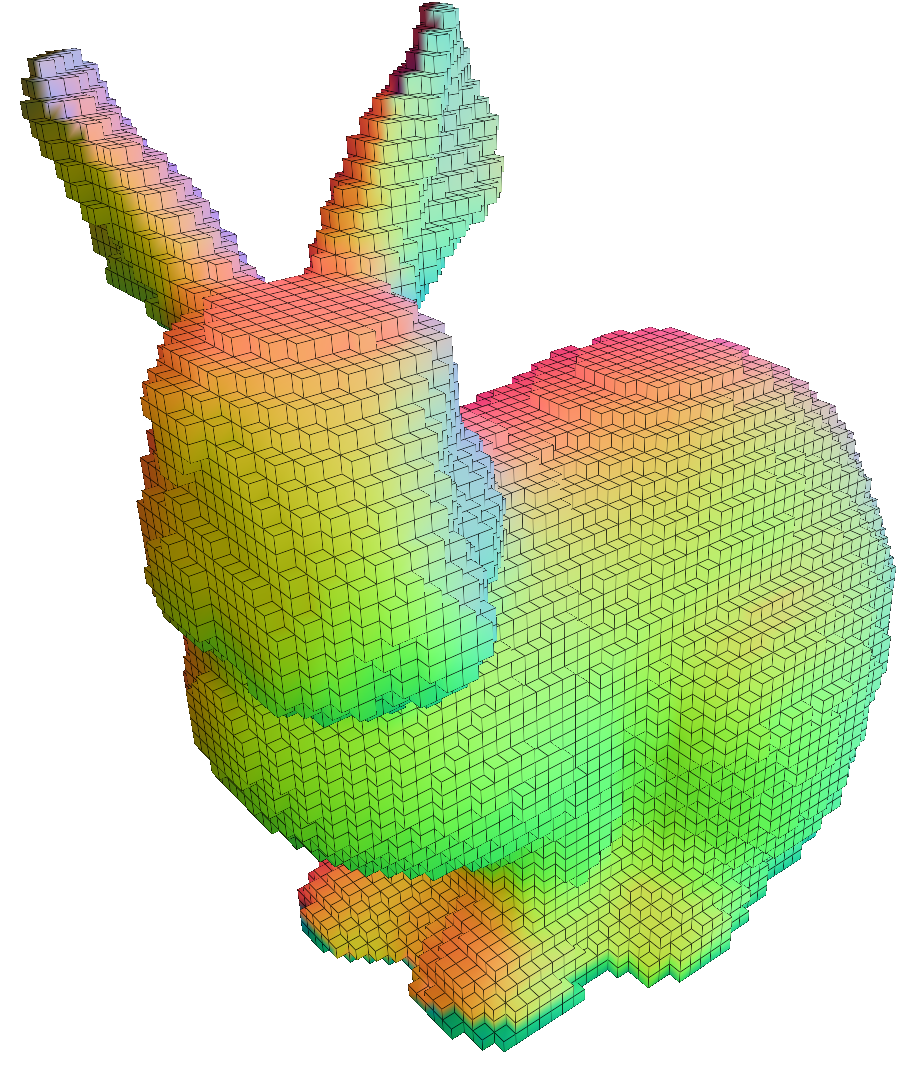
\includegraphics[width=0.45\textwidth]{pictures/normal_digital_surf}
            &
            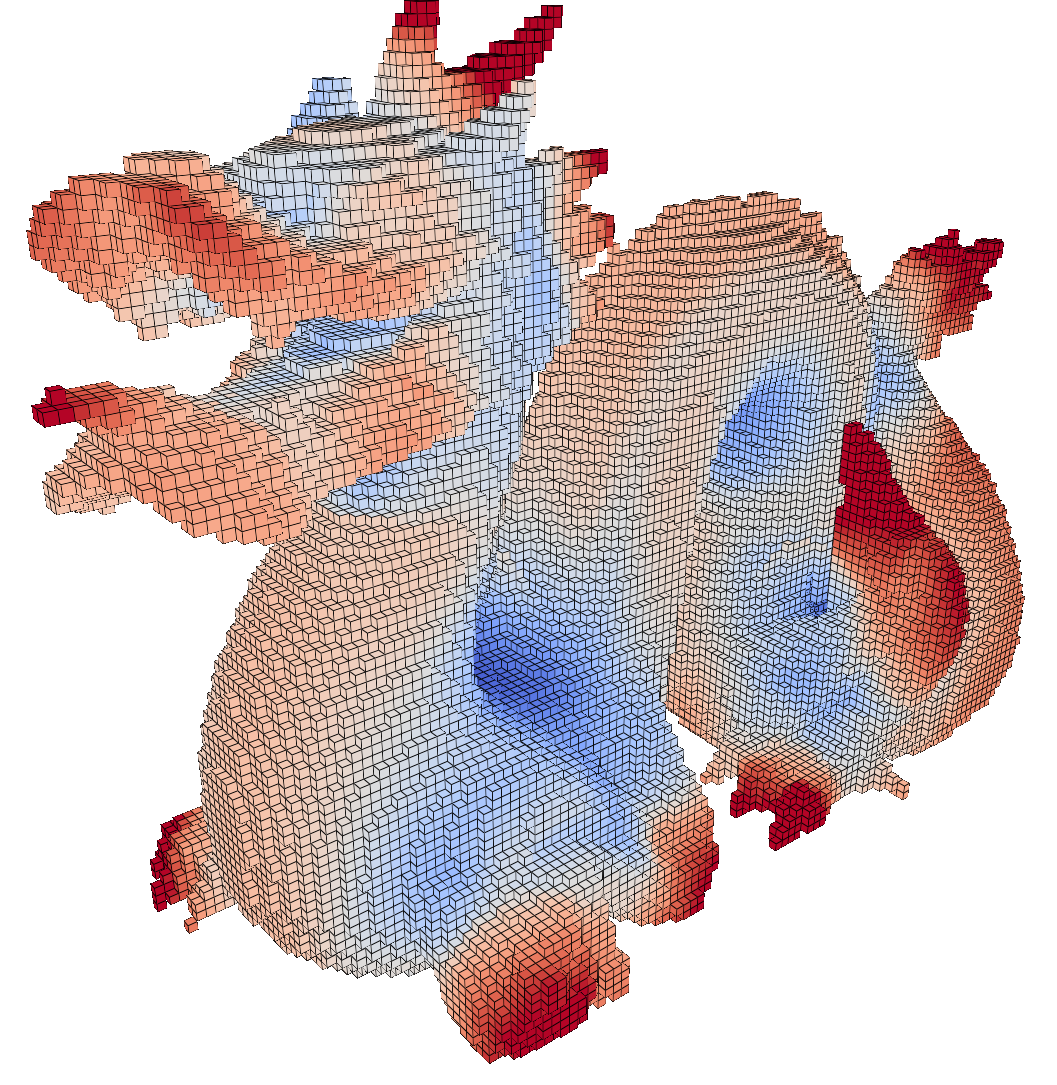
\includegraphics[width=0.45\textwidth]{pictures/Hcurv_digital_surface}
            \\
            Normals as colormap
            &
            Mean Curvature
            \\
            (color(x) = $\frac{1}{2} \times \left(n\left(x\right)+\mathbbm{1}\right)$)
        \end{tabular}
    \end{frame}
    \begin{frame}{Different Types of Digital Surfaces}
        \centering
        \begin{tabular}{|c||c|c|}
            & Smooth Surface & Piecewise-Smooth Surface \\
            \hline
            Implicit surface &
            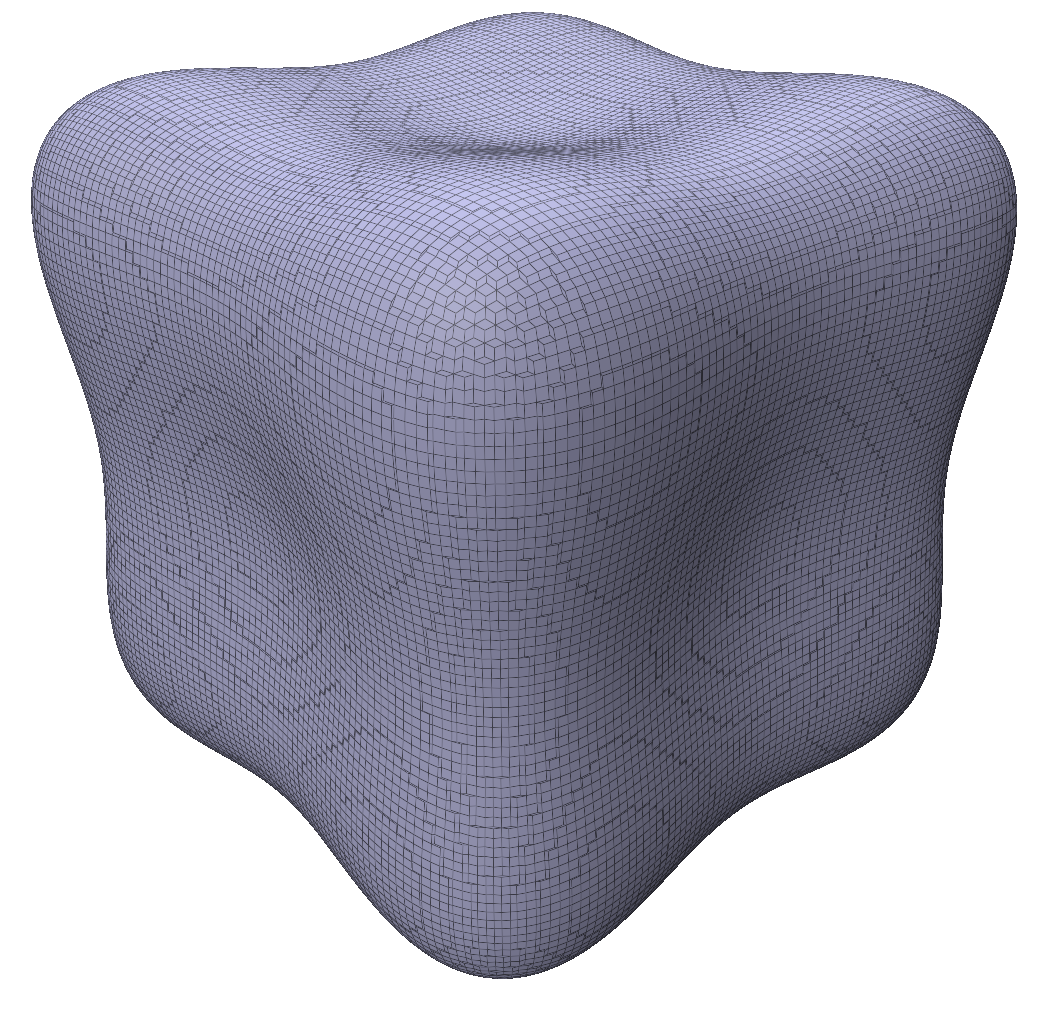
\includegraphics[width=0.25\textwidth]{pictures/smooth_smooth_f3} &
            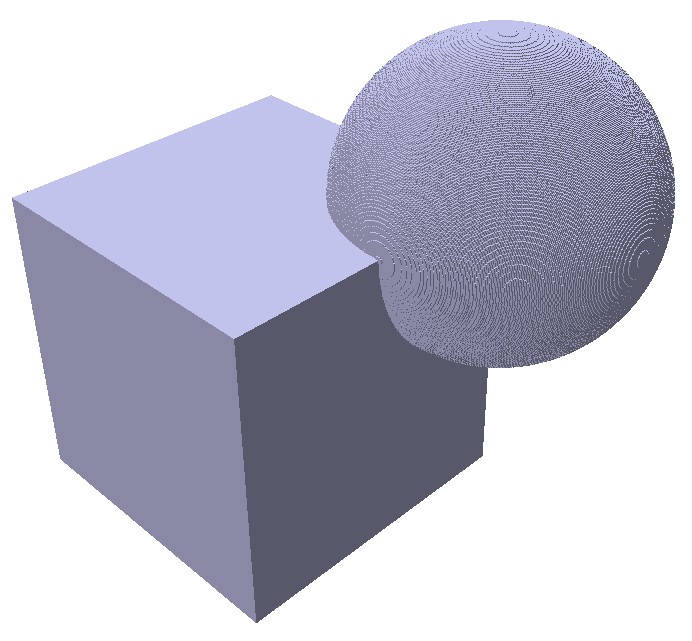
\includegraphics[width=0.25\textwidth]{pictures/piecewise_smooth_smooth_f3} \\
            \hline
            Digitized surface &
            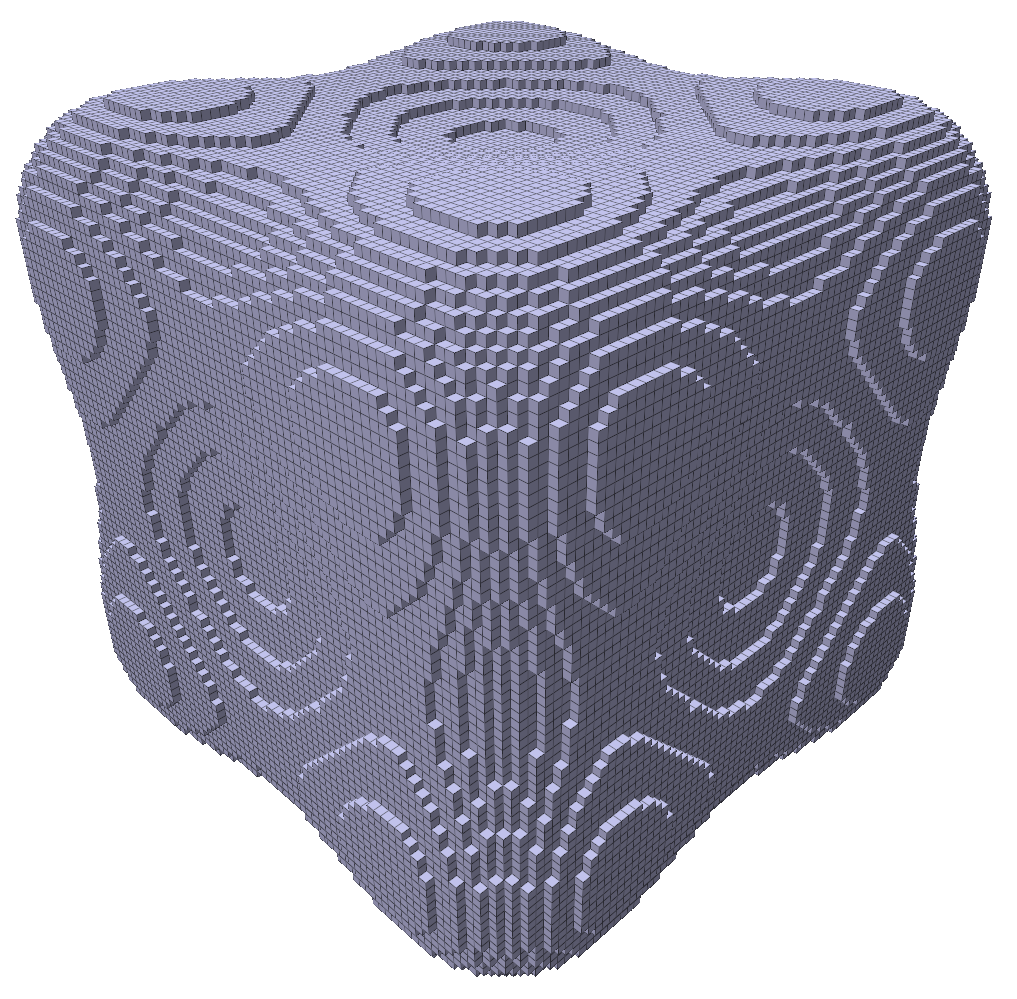
\includegraphics[width=0.25\textwidth]{pictures/smooth_discrete_f3} &
            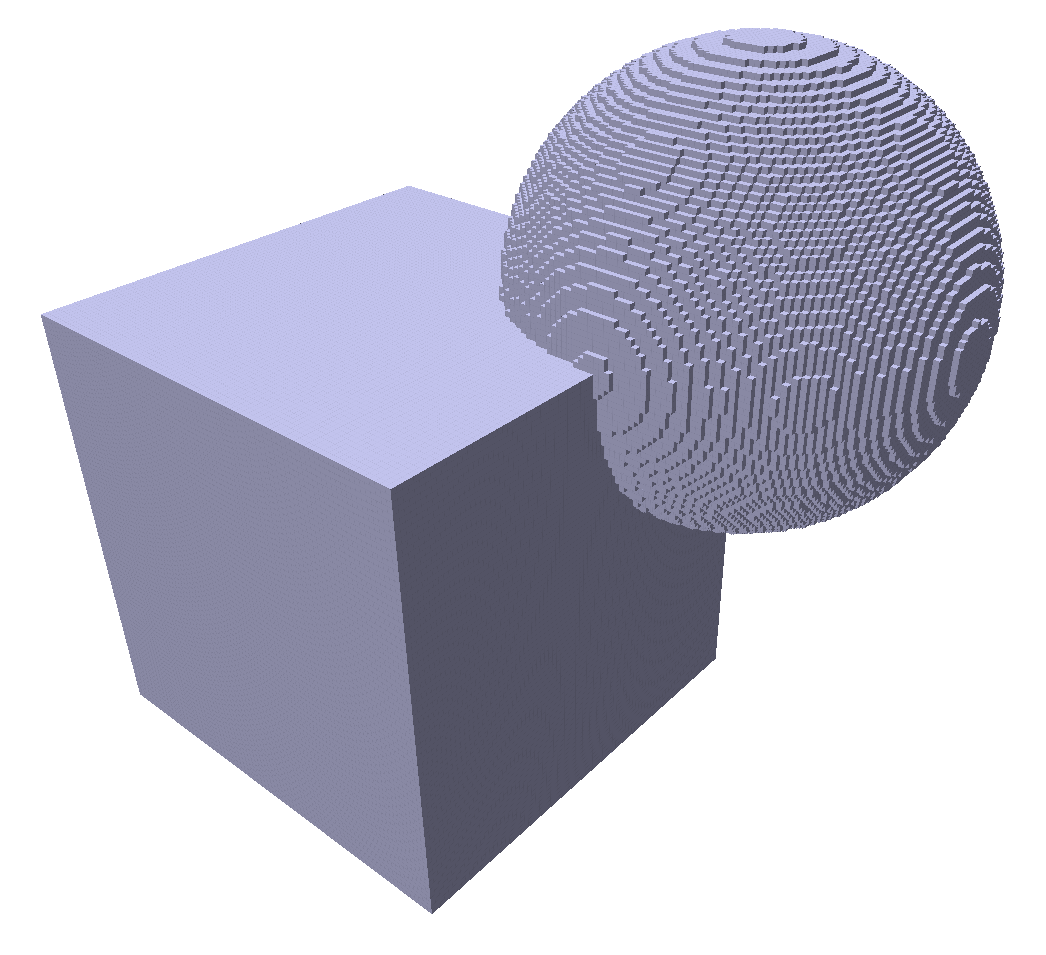
\includegraphics[width=0.25\textwidth]{pictures/piecewise_smooth_discrete_f3} \\
            \hline
        \end{tabular}
        \begin{itemize}
            \item Smooth surfaces — continuous curvature, easy to approximate.
            \item Piecewise-smooth surfaces — sharp features, saliencies, discontinuities.
        \end{itemize}

    \end{frame}
    \begin{frame}{Limitations of Existing Estimators}
        \centering
        \begin{columns}
            \column{0.4\textwidth}
            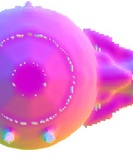
\includegraphics[width=0.85\linewidth]{pictures/tie256-IIN-flat-small-zoomed}
            \column{0.4\textwidth}
            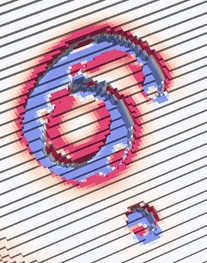
\includegraphics[width=0.85\linewidth]{pictures/d20-H-II-small-zoomed}
        \end{columns}
        \vspace{0.3cm}
        \begin{itemize}
            \item Integral invariant (II) [Lachaud et al., 2017] and Voronoi [Cuel et al., 2014] estimators perform well on smooth areas,
            but fails near saliencies.
            \item Result: normals oscillates across edges, curvature maps show artifacts.
        \end{itemize}
    \end{frame}
    \begin{frame}{Our Objective}
        \begin{itemize}
            \item Develop a parameter-free method.
            \item Respect saliencies and local connectivity.
            \item Provide accurate normals and curvatures on both digitized smooth and digitized piecewise-smooth surfaces.
            \item Keeps a low complexity for practical use.
        \end{itemize}
    \end{frame}

    \begin{frame}{What is the Star of a Shape?}
        \begin{itemize}
            \item Let $X \subset \mathbb{Z}^n$ be a digitized shape.
            \item $Star(X) \coloneqq $ set of all cells incident to $X$
        \end{itemize}
        \vspace{0.3cm}
        \centering
        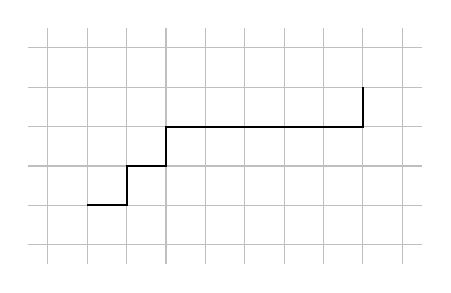
\begin{tikzpicture}
            \draw[step=0.5,lightgray,thin,xshift=-1cm,yshift=-1cm] (0.25,0.25) grid (5.25,3.25);
            \draw[thick] (0,0) -- (0.5,0) -- (0.5,0.5) -- (1,0.5) -- (1,1) -- (3.5,1) -- (3.5,1.5);
        \end{tikzpicture}
    \end{frame}
    \begin{frame}{What is the Star of a Shape?}
        \begin{itemize}
            \item Let $X \subset \mathbb{Z}^n$ be a digitized shape.
            \item $Star(X) \coloneqq $ set of all cells incident to $X$
        \end{itemize}
        \vspace{0.3cm}
        \centering
        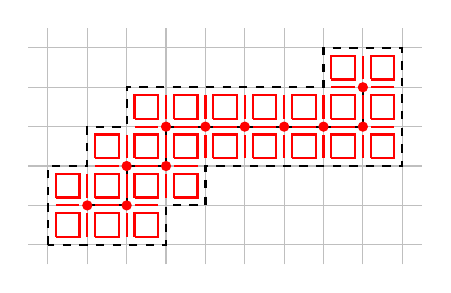
\begin{tikzpicture}
            \draw[step=0.5,lightgray,thin,xshift=-1cm,yshift=-1cm] (0.25,0.25) grid (5.25,3.25);
            \draw[thick,dashed] (-0.5,-0.5) -- (-0.5,0.5) -- (0,0.5) -- (0,1) -- (0.5,1) -- (0.5,1.5) -- (3,1.5) -- (3,2) -- (4,2) -- (4,0.5) -- (1.5,0.5) -- (1.5,0) -- (1,0) -- (1,-0.5) -- (-0.5,-0.5);
            \draw[thick] (0,0) -- (0.5,0) -- (0.5,0.5) -- (1,0.5) -- (1,1) -- (3.5,1) -- (3.5,1.5);

            \drawSquare{-0.5}{-0.5};
            \drawSquare{0}{-0.5};
            \drawSquare{0.5}{-0.5};
            \drawSquare{-0.5}{0};
            \drawSquare{0}{0};
            \drawSquare{0.5}{0};
            \drawSquare{1}{0};
            \drawSquare{0}{0.5};
            \drawSquare{0.5}{0.5};
            \drawSquare{1}{0.5};
            \drawSquare{1.5}{0.5};
            \drawSquare{2}{0.5};
            \drawSquare{2.5}{0.5};
            \drawSquare{3}{0.5};
            \drawSquare{3.5}{0.5};
            \drawSquare{0.5}{1};
            \drawSquare{1}{1};
            \drawSquare{1.5}{1};
            \drawSquare{2}{1};
            \drawSquare{2.5}{1};
            \drawSquare{3}{1};
            \drawSquare{3.5}{1};
            \drawSquare{3}{1.5};
            \drawSquare{3.5}{1.5};

            \drawVLine{0}{-0.5};
            \drawVLine{0}{0};
            \drawVLine{0.5}{-0.5};
            \drawVLine{0.5}{0};
            \drawVLine{0.5}{0.5};
            \drawVLine{1}{0};
            \drawVLine{1}{0.5};
            \drawVLine{1}{1};
            \drawVLine{1.5}{0.5};
            \drawVLine{1.5}{1};
            \drawVLine{2}{0.5};
            \drawVLine{2}{1};
            \drawVLine{2.5}{0.5};
            \drawVLine{2.5}{1};
            \drawVLine{3}{0.5};
            \drawVLine{3}{1};
            \drawVLine{3.5}{0.5};
            \drawVLine{3.5}{1};
            \drawVLine{3.5}{1.5};

            \drawHLine{0}{-0.5};
            \drawHLine{0}{0};
            \drawHLine{0}{0.5};
            \drawHLine{0.5}{0};
            \drawHLine{0.5}{0.5};
            \drawHLine{0.5}{1};
            \drawHLine{1}{0.5};
            \drawHLine{1}{1};
            \drawHLine{1}{1.5};
            \drawHLine{1}{2};
            \drawHLine{1}{2.5};
            \drawHLine{1}{3};
            \drawHLine{1}{3.5};
            \drawHLine{1.5}{3};
            \drawHLine{1.5}{3.5};

            \drawPoint{0}{0};
            \drawPoint{0.5}{0};
            \drawPoint{0.5}{0.5};
            \drawPoint{1}{0.5};
            \drawPoint{1}{1};
            \drawPoint{1.5}{1};
            \drawPoint{2}{1};
            \drawPoint{2.5}{1};
            \drawPoint{3}{1};
            \drawPoint{3.5}{1};
            \drawPoint{3.5}{1.5};

        \end{tikzpicture}
    \end{frame}

    \begin{frame}{What is visibility?}
        \begin{itemize}
            \item Two points on a digital surface are visible from each other if the straight segment connecting them lies entirely within the star of the shape.
            \item It is the digital equivalent of line-of-sight continuity on a smooth manifold.
        \end{itemize}
        \vspace{0.3cm}
        \centering
        \hspace*{-1cm}
        \begin{tabular}{c@{~}|@{~}c@{~}|@{~}c@{~}|@{~}c}
            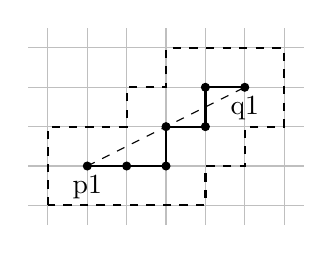
\begin{tikzpicture}
                \draw[step=0.5,lightgray,thin,xshift=-1cm,yshift=-1cm] (0.25,0.25) grid (3.75,2.75);
                \draw[dashed] (0,0) -- (2,1);
                \filldraw[black] (0,0) circle (0.05) node[anchor=north] {p1};
                \filldraw[black] (2,1) circle (0.05) node[anchor=north] {q1};
                \foreach \x/\y in {1/0,2/0,2/1,3/1,3/2} {
                    \filldraw[black] (0.5*\x,0.5*\y) circle (0.05);
                }
                \draw [thick] (0,0) -- (0.5,0) -- (1,0) -- (1,0.5) -- (1.5,0.5) -- (1.5,1) -- (2,1);
                \draw[thick,dashed] (-0.5,-0.5) -- (-0.5,0.5) -- (0.5,0.5) -- (0.5,1) -- (1,1) -- (1,1.5) -- (2.5,1.5) -- (2.5,0.5) -- (2,0.5) -- (2,0) -- (1.5,0) -- (1.5,-0.5) -- (-0.5,-0.5);
            \end{tikzpicture} &
            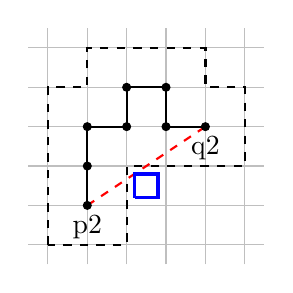
\begin{tikzpicture}
                \draw[step=0.5,lightgray,thin,xshift=-1cm,yshift=-1cm] (0.25,0.25) grid (3.25,3.25);
                \draw[red,dashed,thick] (0,0) -- (1.5,1);
                \filldraw[black] (0,0) circle (0.05) node[anchor=north] {p2};
                \filldraw[black] (1.5,1) circle (0.05) node[anchor=north] {q2};
                \foreach \x/\y in {0/1,0/2,1/2,1/3,2/3,2/2} {
                    \filldraw[black] (0.5*\x,0.5*\y) circle (0.05);
                }
                \draw [thick] (0,0) -- (0,1) -- (0.5,1) -- (0.5,1.5) -- (1,1.5) -- (1,1) -- (1.5,1);
                \draw[thick,dashed] (-0.5,-0.5) -- (-0.5,1.5) -- (0,1.5) -- (0,2) -- (1.5,2) -- (1.5,1.5) -- (2,1.5)  -- (2,0.5) -- (0.5,0.5) -- (0.5,-0.5) -- (-0.5,-0.5);
                \draw[very thick, blue] (0.5+0.1,0+0.1) -- (0.5+0.4,0+0.1) -- (0.5+0.4,0+0.4) -- (0.5+0.1,0+0.4) -- (0.5+0.1,0+0.1);
            \end{tikzpicture} &
            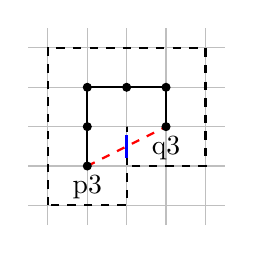
\begin{tikzpicture}
                \draw[step=0.5,lightgray,thin,xshift=-1cm,yshift=-1cm] (0.25,0.25) grid (2.75,2.75);
                \draw[red,dashed,thick] (0,0) -- (1,0.5);
                \filldraw[black] (0,0) circle (0.05) node[anchor=north] {p3};
                \filldraw[black] (1,0.5) circle (0.05) node[anchor=north] {q3};
                \foreach \x/\y in {0/1,0/2,1/2,2/2} {
                    \filldraw[black] (0.5*\x,0.5*\y) circle (0.05);
                }
                \draw [thick] (0,0) -- (0,1) -- (1,1) -- (1,0.5);
                \draw[thick,dashed] (-0.5,-0.5) -- (-0.5,1.5) -- (1.5,1.5) -- (1.5,0) -- (0.5,0) -- (0.5,0.5) -- (0.5,-0.5) -- (-0.5,-0.5);
                \draw[very thick, blue] (0.5,0+0.1) -- (0.5,0+0.4);
            \end{tikzpicture} &
            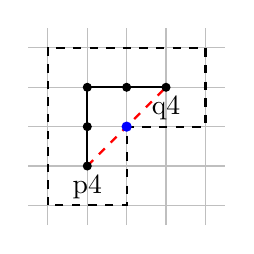
\begin{tikzpicture}
                \draw[step=0.5,lightgray,thin,xshift=-1cm,yshift=-1cm] (0.25,0.25) grid (2.75,2.75);
                \draw[red,dashed,thick] (0,0) -- (1,1);
                \filldraw[black] (0,0) circle (0.05) node[anchor=north] {p4};
                \filldraw[black] (1,1) circle (0.05) node[anchor=north] {q4};
                \foreach \x/\y in {0/1,0/2,1/2} {
                    \filldraw[black] (0.5*\x,0.5*\y) circle (0.05);
                }
                \draw [thick] (0,0) -- (0,1) -- (1,1);
                \draw[thick,dashed] (-0.5,-0.5) -- (-0.5,1.5) -- (1.5,1.5) -- (1.5,0.5) -- (0.5,0.5) -- (0.5,-0.5) -- (-0.5,-0.5);
                \filldraw[thick, blue] (0.5,0.5) circle (0.05);
            \end{tikzpicture} \\
            Visible & Non-Visible &
            Non-Visible & Non-Visible
        \end{tabular}
    \end{frame}

    \begin{frame}{Visibility set may be non-connex}
        \begin{itemize}
            \item The set of points visible from a given surface point is not necessarily connected.
            \item Breaks assumptions made by region-growing or BFS-based algorithms.
            \item Handling non-connex visibility sets requires an exact representation
            \item Need of a specific structure with specific algorithms.
        \end{itemize}
        \vspace{0.3cm}
        \centering
        \begin{figure}[t]
            \centering
            \begin{tikzpicture}
                \draw[step=0.5,lightgray,thin,xshift=-1cm,yshift=-1cm] (0.25,0.25) grid (5.25,3.25);
                \draw[thick] (0,0) -- (0.5,0) -- (0.5,0.5) -- (1,0.5) -- (1,1) -- (3.5,1) -- (3.5,1.5);
                \draw [black, dashed] (0,0) -- (3.5,1.5);
                \draw [red, dashed] (0,0) -- (3.5,1);
                \draw [red, dashed] (0,0) -- (3,1);
                \filldraw[black] (0,0) circle (0.05) node[anchor=north] {p};
                \filldraw[gray] (0.5,0) circle (0.05);
                \filldraw[gray] (0.5,0.5) circle (0.05);
                \filldraw[gray] (1,0.5) circle (0.05);
                \filldraw[gray] (1,1) circle (0.05);
                \filldraw[gray] (1.5,1) circle (0.05);
                \filldraw[gray] (2,1) circle (0.05);
                \filldraw[gray] (2.5,1) circle (0.05);
                \filldraw[red] (3,1) circle (0.05);
                \filldraw[red] (3.5,1) circle (0.05);
                \filldraw[black] (3.5,1.5) circle (0.05) node[anchor=west] {q};
                \draw[thick,dashed] (-0.5,-0.5) -- (-0.5,0.5) -- (0,0.5) -- (0,1) -- (0.5,1) -- (0.5,1.5) -- (3,1.5) -- (3,2) -- (4,2) -- (4,0.5) -- (1.5,0.5) -- (1.5,0) -- (1,0) -- (1,-0.5) -- (-0.5,-0.5);
                \draw[very thick, blue] (1.5+0.1,0+0.1) -- (1.5+0.4,0+0.1) -- (1.5+0.4,0+0.4) -- (1.5+0.1,0+0.4) -- (1.5+0.1,0+0.1);
                \filldraw[thick, blue] (1.5,0.5) circle (0.05);
                \draw[thick, blue] (1.5,0+0.1) -- (1.5,0+0.4)
                \draw[thick, blue] (1.5+0.1,0.5) -- (1.5+0.4,0.5)
            \end{tikzpicture}
            \label{fig:visibility-2d-not-connected}
        \end{figure}
    \end{frame}


    \section{Representing the star of a shape}

    \begin{frame}{Representing the star of a shape}
        \begin{itemize}
            \item Current Star
        \end{itemize}
        \vspace{0.2cm}
        \centering
        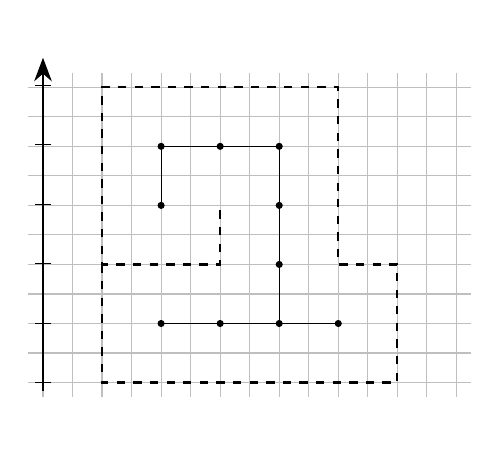
\begin{tikzpicture}[scale=0.75]
            \draw[step=0.5,lightgray,thin,xshift=-1cm,yshift=-1cm] (-0.25,1.75) grid (7.25,7.25);
            \filldraw[black] (1,4) circle (0.05);
            \filldraw[black] (1,5) circle (0.05);
            \filldraw[black] (2,5) circle (0.05);
            \filldraw[black] (3,5) circle (0.05);
            \filldraw[black] (3,4) circle (0.05);
            \filldraw[black] (3,3) circle (0.05);
            \filldraw[black] (3,2) circle (0.05);
            \filldraw[black] (2,2) circle (0.05);
            \filldraw[black] (1,2) circle (0.05);
            \filldraw[black] (4,2) circle (0.05);
            \draw[-{Stealth[length=3mm]}=black] (-1,1) -- (-1,6.5);
            \draw decorate [decoration={crosses,transform={rotate=45},shape size=1.5mm,segment length=21.5pt}] {(-1,1) -- (-1,7)};
            \draw[black] (1,4) -- (1,5) -- (3,5) -- (3,2) -- (4,2) -- (1,2) ;
            \draw[thick,dashed]  (0,3) -- (0,1) -- (5,1) -- (5,3) -- (4,3) -- (4,6) -- (0,6) -- (0,3) -- (2,3) -- (2,4);
        \end{tikzpicture}
    \end{frame}
    \begin{frame}{Representing the star of a shape}
        \begin{itemize}
            \item Current Star
        \end{itemize}
        \vspace{0.2cm}
        \centering
        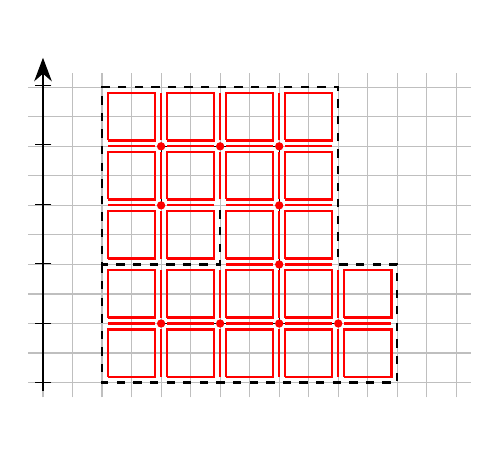
\begin{tikzpicture}[scale=0.75]
            \draw[step=0.5,lightgray,thin,xshift=-1cm,yshift=-1cm] (-0.25,1.75) grid (7.25,7.25);
            \filldraw[black] (1,4) circle (0.05);
            \filldraw[black] (1,5) circle (0.05);
            \filldraw[black] (2,5) circle (0.05);
            \filldraw[black] (3,5) circle (0.05);
            \filldraw[black] (3,4) circle (0.05);
            \filldraw[black] (3,3) circle (0.05);
            \filldraw[black] (3,2) circle (0.05);
            \filldraw[black] (2,2) circle (0.05);
            \filldraw[black] (1,2) circle (0.05);
            \filldraw[black] (4,2) circle (0.05);
            \draw[-{Stealth[length=3mm]}=black] (-1,1) -- (-1,6.5);
            \draw decorate [decoration={crosses,transform={rotate=45},shape size=1.5mm,segment length=21.5pt}] {(-1,1) -- (-1,7)};
            \draw[black] (1,4) -- (1,5) -- (3,5) -- (3,2) -- (4,2) -- (1,2) ;
            \draw[thick,dashed]  (0,3) -- (0,1) -- (5,1) -- (5,3) -- (4,3) -- (4,6) -- (0,6) -- (0,3) -- (2,3) -- (2,4);

            \drawBigSquare{-1}{-1};
            \drawBigSquare{-1}{0};
            \drawBigSquare{-1}{1};
            \drawBigSquare{-1}{2};
            \drawBigSquare{-1}{3};
            \drawBigSquare{0}{-1};
            \drawBigSquare{0}{0};
            \drawBigSquare{0}{1};
            \drawBigSquare{0}{2};
            \drawBigSquare{0}{3};
            \drawBigSquare{1}{-1};
            \drawBigSquare{1}{0};
            \drawBigSquare{1}{1};
            \drawBigSquare{1}{2};
            \drawBigSquare{1}{3};
            \drawBigSquare{2}{-1};
            \drawBigSquare{2}{0};
            \drawBigSquare{2}{1};
            \drawBigSquare{2}{2};
            \drawBigSquare{2}{3};
            \drawBigSquare{3}{-1};
            \drawBigSquare{3}{0};

            \drawBigVLine{0}{-1};
            \drawBigVLine{0}{0};
            \drawBigVLine{0}{1};
            \drawBigVLine{0}{2};
            \drawBigVLine{0}{3};
            \drawBigVLine{1}{-1};
            \drawBigVLine{1}{0};
            \drawBigVLine{1}{2};
            \drawBigVLine{1}{3};
            \drawBigVLine{2}{-1};
            \drawBigVLine{2}{0};
            \drawBigVLine{2}{1};
            \drawBigVLine{2}{2};
            \drawBigVLine{2}{3};
            \drawBigVLine{3}{-1};
            \drawBigVLine{3}{0};

            \drawBigHLine{-1}{0};
            \drawBigHLine{-1}{2};
            \drawBigHLine{-1}{3};
            \drawBigHLine{0}{0};
            \drawBigHLine{0}{2};
            \drawBigHLine{0}{3};
            \drawBigHLine{1}{0};
            \drawBigHLine{1}{1};
            \drawBigHLine{1}{2};
            \drawBigHLine{1}{3};
            \drawBigHLine{2}{0};
            \drawBigHLine{2}{1};
            \drawBigHLine{2}{2};
            \drawBigHLine{2}{3};
            \drawBigHLine{3}{0};

            \drawPoint{1}{4};
            \drawPoint{1}{5};
            \drawPoint{2}{5};
            \drawPoint{3}{5};
            \drawPoint{3}{4};
            \drawPoint{3}{3};
            \drawPoint{3}{2};
            \drawPoint{2}{2};
            \drawPoint{1}{2};
            \drawPoint{4}{2};
        \end{tikzpicture}
    \end{frame}
    \begin{frame}{Representing the star of a shape}
        \begin{itemize}
            \item One cell = one coordinate
        \end{itemize}
        \vspace{0.2cm}
        \centering
        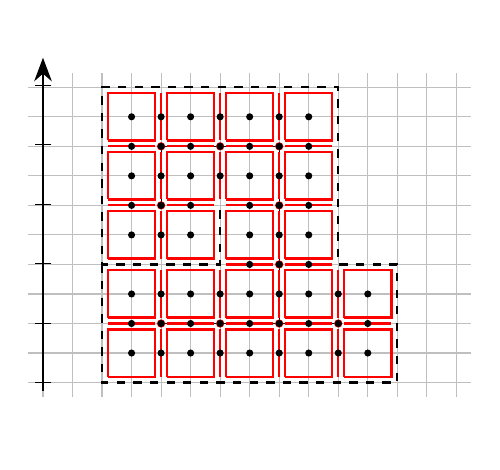
\begin{tikzpicture}[scale=0.75]
            \draw[step=0.5,lightgray,thin,xshift=-1cm,yshift=-1cm] (-0.25,1.75) grid (7.25,7.25);
            \filldraw[black] (1,4) circle (0.05);
            \filldraw[black] (1,5) circle (0.05);
            \filldraw[black] (2,5) circle (0.05);
            \filldraw[black] (3,5) circle (0.05);
            \filldraw[black] (3,4) circle (0.05);
            \filldraw[black] (3,3) circle (0.05);
            \filldraw[black] (3,2) circle (0.05);
            \filldraw[black] (2,2) circle (0.05);
            \filldraw[black] (1,2) circle (0.05);
            \filldraw[black] (4,2) circle (0.05);
            \draw[-{Stealth[length=3mm]}=black] (-1,1) -- (-1,6.5);
            \draw decorate [decoration={crosses,transform={rotate=45},shape size=1.5mm,segment length=21.5pt}] {(-1,1) -- (-1,7)};
            \draw[black] (1,4) -- (1,5) -- (3,5) -- (3,2) -- (4,2) -- (1,2) ;
            \draw[thick,dashed]  (0,3) -- (0,1) -- (5,1) -- (5,3) -- (4,3) -- (4,6) -- (0,6) -- (0,3) -- (2,3) -- (2,4);

            \drawBigSquare{-1}{-1};
            \drawBigSquare{-1}{0};
            \drawBigSquare{-1}{1};
            \drawBigSquare{-1}{2};
            \drawBigSquare{-1}{3};
            \drawBigSquare{0}{-1};
            \drawBigSquare{0}{0};
            \drawBigSquare{0}{1};
            \drawBigSquare{0}{2};
            \drawBigSquare{0}{3};
            \drawBigSquare{1}{-1};
            \drawBigSquare{1}{0};
            \drawBigSquare{1}{1};
            \drawBigSquare{1}{2};
            \drawBigSquare{1}{3};
            \drawBigSquare{2}{-1};
            \drawBigSquare{2}{0};
            \drawBigSquare{2}{1};
            \drawBigSquare{2}{2};
            \drawBigSquare{2}{3};
            \drawBigSquare{3}{-1};
            \drawBigSquare{3}{0};

            \drawBigVLine{0}{-1};
            \drawBigVLine{0}{0};
            \drawBigVLine{0}{1};
            \drawBigVLine{0}{2};
            \drawBigVLine{0}{3};
            \drawBigVLine{1}{-1};
            \drawBigVLine{1}{0};
            \drawBigVLine{1}{2};
            \drawBigVLine{1}{3};
            \drawBigVLine{2}{-1};
            \drawBigVLine{2}{0};
            \drawBigVLine{2}{1};
            \drawBigVLine{2}{2};
            \drawBigVLine{2}{3};
            \drawBigVLine{3}{-1};
            \drawBigVLine{3}{0};

            \drawBigHLine{-1}{0};
            \drawBigHLine{-1}{2};
            \drawBigHLine{-1}{3};
            \drawBigHLine{0}{0};
            \drawBigHLine{0}{2};
            \drawBigHLine{0}{3};
            \drawBigHLine{1}{0};
            \drawBigHLine{1}{1};
            \drawBigHLine{1}{2};
            \drawBigHLine{1}{3};
            \drawBigHLine{2}{0};
            \drawBigHLine{2}{1};
            \drawBigHLine{2}{2};
            \drawBigHLine{2}{3};
            \drawBigHLine{3}{0};

            \drawPoint{1}{4};
            \drawPoint{1}{5};
            \drawPoint{2}{5};
            \drawPoint{3}{5};
            \drawPoint{3}{4};
            \drawPoint{3}{3};
            \drawPoint{3}{2};
            \drawPoint{2}{2};
            \drawPoint{1}{2};
            \drawPoint{4}{2};


            \drawBlackPointSquare{-1}{-1};
            \drawBlackPointSquare{-1}{0};
            \drawBlackPointSquare{-1}{1};
            \drawBlackPointSquare{-1}{2};
            \drawBlackPointSquare{-1}{3};
            \drawBlackPointSquare{0}{-1};
            \drawBlackPointSquare{0}{0};
            \drawBlackPointSquare{0}{1};
            \drawBlackPointSquare{0}{2};
            \drawBlackPointSquare{0}{3};
            \drawBlackPointSquare{1}{-1};
            \drawBlackPointSquare{1}{0};
            \drawBlackPointSquare{1}{1};
            \drawBlackPointSquare{1}{2};
            \drawBlackPointSquare{1}{3};
            \drawBlackPointSquare{2}{-1};
            \drawBlackPointSquare{2}{0};
            \drawBlackPointSquare{2}{1};
            \drawBlackPointSquare{2}{2};
            \drawBlackPointSquare{2}{3};
            \drawBlackPointSquare{3}{-1};
            \drawBlackPointSquare{3}{0};

            \drawBlackPointVLine{0}{-1};
            \drawBlackPointVLine{0}{0};
            \drawBlackPointVLine{0}{1};
            \drawBlackPointVLine{0}{2};
            \drawBlackPointVLine{0}{3};
            \drawBlackPointVLine{1}{-1};
            \drawBlackPointVLine{1}{0};
            \drawBlackPointVLine{1}{2};
            \drawBlackPointVLine{1}{3};
            \drawBlackPointVLine{2}{-1};
            \drawBlackPointVLine{2}{0};
            \drawBlackPointVLine{2}{1};
            \drawBlackPointVLine{2}{2};
            \drawBlackPointVLine{2}{3};
            \drawBlackPointVLine{3}{-1};
            \drawBlackPointVLine{3}{0};

            \drawBlackPointHline{-1}{0};
            \drawBlackPointHline{-1}{2};
            \drawBlackPointHline{-1}{3};
            \drawBlackPointHline{0}{0};
            \drawBlackPointHline{0}{2};
            \drawBlackPointHline{0}{3};
            \drawBlackPointHline{1}{0};
            \drawBlackPointHline{1}{1};
            \drawBlackPointHline{1}{2};
            \drawBlackPointHline{1}{3};
            \drawBlackPointHline{2}{0};
            \drawBlackPointHline{2}{1};
            \drawBlackPointHline{2}{2};
            \drawBlackPointHline{2}{3};
            \drawBlackPointHline{3}{0};

            \drawBlackPointPoint{1}{4};
            \drawBlackPointPoint{1}{5};
            \drawBlackPointPoint{2}{5};
            \drawBlackPointPoint{3}{5};
            \drawBlackPointPoint{3}{4};
            \drawBlackPointPoint{3}{3};
            \drawBlackPointPoint{3}{2};
            \drawBlackPointPoint{2}{2};
            \drawBlackPointPoint{1}{2};
            \drawBlackPointPoint{4}{2};


        \end{tikzpicture}
    \end{frame}
    \begin{frame}{Representing the star of a shape}
        \begin{itemize}
            \item List of integer intervals.
        \end{itemize}
        \vspace{0.2cm}
        \centering
        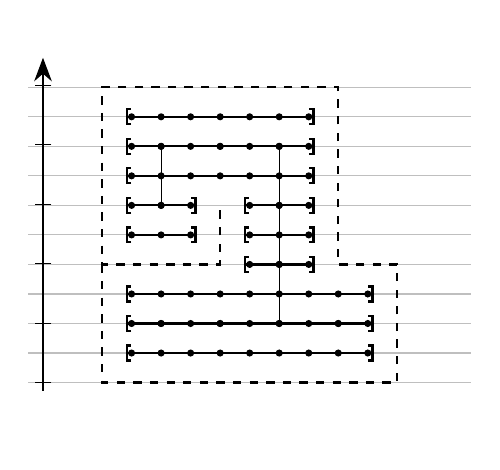
\begin{tikzpicture}[scale=0.75]
            \foreach \y in {2,2.5,...,7} {
                \draw[thin, lightgray,xshift=-1cm,yshift=-1cm] (-0.25,\y) -- (7.25,\y);
            }
            \filldraw[black] (1,4) circle (0.05);
            \filldraw[black] (1,5) circle (0.05);
            \filldraw[black] (2,5) circle (0.05);
            \filldraw[black] (3,5) circle (0.05);
            \filldraw[black] (3,4) circle (0.05);
            \filldraw[black] (3,3) circle (0.05);
            \filldraw[black] (3,2) circle (0.05);
            \filldraw[black] (2,2) circle (0.05);
            \filldraw[black] (1,2) circle (0.05);
            \filldraw[black] (4,2) circle (0.05);
            \draw[-{Stealth[length=3mm]}=black] (-1,1) -- (-1,6.5);
            \draw decorate [decoration={crosses,transform={rotate=45},shape size=1.5mm,segment length=21.5pt}] {(-1,1) -- (-1,7)};
            \draw[black] (1,4) -- (1,5) -- (3,5) -- (3,2) -- (4,2) -- (1,2) ;
            \draw[thick,dashed]  (0,3) -- (0,1) -- (5,1) -- (5,3) -- (4,3) -- (4,6) -- (0,6) -- (0,3) -- (2,3) -- (2,4);

            \drawBlackPointSquare{-1}{-1};
            \drawBlackPointSquare{-1}{0};
            \drawBlackPointSquare{-1}{1};
            \drawBlackPointSquare{-1}{2};
            \drawBlackPointSquare{-1}{3};
            \drawBlackPointSquare{0}{-1};
            \drawBlackPointSquare{0}{0};
            \drawBlackPointSquare{0}{1};
            \drawBlackPointSquare{0}{2};
            \drawBlackPointSquare{0}{3};
            \drawBlackPointSquare{1}{-1};
            \drawBlackPointSquare{1}{0};
            \drawBlackPointSquare{1}{1};
            \drawBlackPointSquare{1}{2};
            \drawBlackPointSquare{1}{3};
            \drawBlackPointSquare{2}{-1};
            \drawBlackPointSquare{2}{0};
            \drawBlackPointSquare{2}{1};
            \drawBlackPointSquare{2}{2};
            \drawBlackPointSquare{2}{3};
            \drawBlackPointSquare{3}{-1};
            \drawBlackPointSquare{3}{0};

            \drawBlackPointVLine{0}{-1};
            \drawBlackPointVLine{0}{0};
            \drawBlackPointVLine{0}{1};
            \drawBlackPointVLine{0}{2};
            \drawBlackPointVLine{0}{3};
            \drawBlackPointVLine{1}{-1};
            \drawBlackPointVLine{1}{0};
            \drawBlackPointVLine{1}{2};
            \drawBlackPointVLine{1}{3};
            \drawBlackPointVLine{2}{-1};
            \drawBlackPointVLine{2}{0};
            \drawBlackPointVLine{2}{1};
            \drawBlackPointVLine{2}{2};
            \drawBlackPointVLine{2}{3};
            \drawBlackPointVLine{3}{-1};
            \drawBlackPointVLine{3}{0};

            \drawBlackPointHline{-1}{0};
            \drawBlackPointHline{-1}{2};
            \drawBlackPointHline{-1}{3};
            \drawBlackPointHline{0}{0};
            \drawBlackPointHline{0}{2};
            \drawBlackPointHline{0}{3};
            \drawBlackPointHline{1}{0};
            \drawBlackPointHline{1}{1};
            \drawBlackPointHline{1}{2};
            \drawBlackPointHline{1}{3};
            \drawBlackPointHline{2}{0};
            \drawBlackPointHline{2}{1};
            \drawBlackPointHline{2}{2};
            \drawBlackPointHline{2}{3};
            \drawBlackPointHline{3}{0};

            \drawBlackPointPoint{1}{4};
            \drawBlackPointPoint{1}{5};
            \drawBlackPointPoint{2}{5};
            \drawBlackPointPoint{3}{5};
            \drawBlackPointPoint{3}{4};
            \drawBlackPointPoint{3}{3};
            \drawBlackPointPoint{3}{2};
            \drawBlackPointPoint{2}{2};
            \drawBlackPointPoint{1}{2};
            \drawBlackPointPoint{4}{2};

            \draw[thick, arrows = {Bracket[sharp]-Bracket[sharp]}] (0.4,5.5)--(3.6,5.5);
            \draw[thick, arrows = {Bracket[sharp]-Bracket[sharp]}] (0.4,5)--(3.6,5);
            \draw[thick, arrows = {Bracket[sharp]-Bracket[sharp]}] (0.4,4.5)--(3.6,4.5);
            \draw[thick, arrows = {Bracket[sharp]-Bracket[sharp]}] (0.4,4)--(1.6,4);
            \draw[thick, arrows = {Bracket[sharp]-Bracket[sharp]}] (2.4,4)--(3.6,4);
            \draw[thick, arrows = {Bracket[sharp]-Bracket[sharp]}] (0.4,3.5)--(1.6,3.5);
            \draw[thick, arrows = {Bracket[sharp]-Bracket[sharp]}] (2.4,3.5)--(3.6,3.5);
            \draw[thick, arrows = {Bracket[sharp]-Bracket[sharp]}] (2.4,3)--(3.6,3);
            \draw[thick, arrows = {Bracket[sharp]-Bracket[sharp]}] (0.4,2.5)--(4.6,2.5);
            \draw[thick, arrows = {Bracket[sharp]-Bracket[sharp]}] (0.4,2)--(4.6,2);
            \draw[thick, arrows = {Bracket[sharp]-Bracket[sharp]}] (0.4,1.5)--(4.6,1.5);


        \end{tikzpicture}
    \end{frame}
    \begin{frame}{Representing the star of a shape}
        \begin{itemize}
            \item 63 cells coordinates -> 11 integer intervals.
        \end{itemize}
        \vspace{0.2cm}
        \centering
        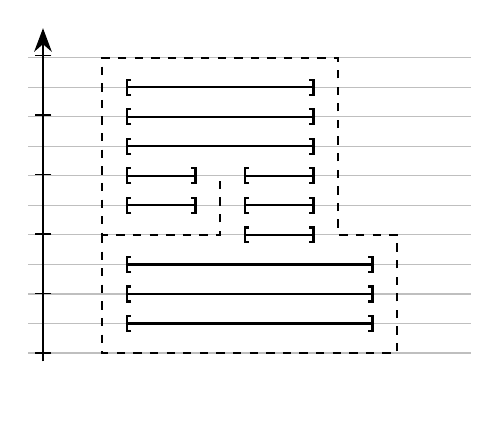
\begin{tikzpicture}[scale=0.75]
            \foreach \y in {2,2.5,...,7} {
                \draw[thin, lightgray,xshift=-1cm,yshift=-1cm] (-0.25,\y) -- (7.25,\y);
            }
            \draw[-{Stealth[length=3mm]}=black] (-1,1) -- (-1,6.5);
            \draw decorate [decoration={crosses,transform={rotate=45},shape size=1.5mm,segment length=21.5pt}] {(-1,1) -- (-1,6.5)};
            \draw[thick,dashed]  (0,3) -- (0,1) -- (5,1) -- (5,3) -- (4,3) -- (4,6) -- (0,6) -- (0,3) -- (2,3) -- (2,4);
            \draw[thick, arrows = {Bracket[sharp]-Bracket[sharp]}] (0.4,5.5)--(3.6,5.5);
            \draw[thick, arrows = {Bracket[sharp]-Bracket[sharp]}] (0.4,5)--(3.6,5);
            \draw[thick, arrows = {Bracket[sharp]-Bracket[sharp]}] (0.4,4.5)--(3.6,4.5);
            \draw[thick, arrows = {Bracket[sharp]-Bracket[sharp]}] (0.4,4)--(1.6,4);
            \draw[thick, arrows = {Bracket[sharp]-Bracket[sharp]}] (2.4,4)--(3.6,4);
            \draw[thick, arrows = {Bracket[sharp]-Bracket[sharp]}] (0.4,3.5)--(1.6,3.5);
            \draw[thick, arrows = {Bracket[sharp]-Bracket[sharp]}] (2.4,3.5)--(3.6,3.5);
            \draw[thick, arrows = {Bracket[sharp]-Bracket[sharp]}] (2.4,3)--(3.6,3);
            \draw[thick, arrows = {Bracket[sharp]-Bracket[sharp]}] (0.4,2.5)--(4.6,2.5);
            \draw[thick, arrows = {Bracket[sharp]-Bracket[sharp]}] (0.4,2)--(4.6,2);
            \draw[thick, arrows = {Bracket[sharp]-Bracket[sharp]}] (0.4,1.5)--(4.6,1.5);
        \end{tikzpicture}
    \end{frame}


    \section{Computing the visibility}
    \begin{frame}{Computing the visibility}
        \vspace{5em}
        \centering
        \hspace*{-2em}
        \begin{tabular}{c c}
            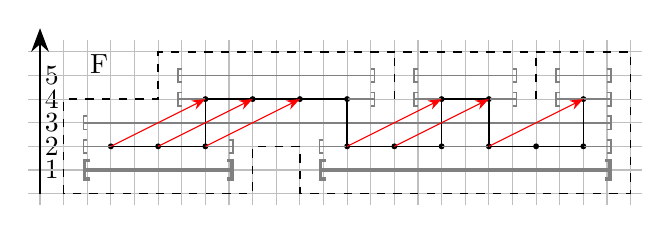
\begin{tikzpicture}[scale=0.6]
                \foreach[count=\i] \y in {-0.5,0,...,1.5} {
                    \draw (0,0) node at (-1.25,\y) {\i};
                }
                \draw[step=0.5,lightgray,thin,xshift=-1cm,yshift=-1cm] (-0.75,-0.25) grid (12.25,3.25);
                \draw[-{Stealth[length=3mm]}=black] (-1.5,-1) -- (-1.5,2.5);
                \filldraw[black] (0,0) circle (0.05);
                \filldraw[black] (1,0) circle (0.05);
                \filldraw[black] (2,0) circle (0.05);
                \filldraw[black] (2,1) circle (0.05);
                \filldraw[black] (3,1) circle (0.05);
                \filldraw[black] (4,1) circle (0.05);
                \filldraw[black] (5,1) circle (0.05);
                \filldraw[black] (5,0) circle (0.05);
                \filldraw[black] (6,0) circle (0.05);
                \filldraw[black] (7,0) circle (0.05);
                \filldraw[black] (7,1) circle (0.05);
                \filldraw[black] (8,1) circle (0.05);
                \filldraw[black] (8,0) circle (0.05);
                \filldraw[black] (9,0) circle (0.05);
                \filldraw[black] (10,0) circle (0.05);
                \filldraw[black] (10,1) circle (0.05);
                \draw[very thick,gray, arrows = {Bracket[sharp]-Bracket[sharp]}] (-0.6,-0.5)--(2.6,-0.5);
                \draw[very thick,gray, arrows = {Bracket[sharp]-Bracket[sharp]}] (4.4,-0.5)--(10.6,-0.5);
                \draw[semithick,gray, arrows = {Bracket[sharp]-Bracket[sharp]}] (-0.6,0)--(2.6,0);
                \draw[semithick,gray, arrows = {Bracket[sharp]-Bracket[sharp]}] (4.4,0)--(10.6,0);
                \draw[semithick,gray, arrows = {Bracket[sharp]-Bracket[sharp]}] (-0.6,0.5)--(10.6,0.5);
                \draw[semithick,gray, arrows = {Bracket[sharp]-Bracket[sharp]}] (1.4,1)--(5.6,1);
                \draw[semithick,gray, arrows = {Bracket[sharp]-Bracket[sharp]}] (6.4,1)--(8.6,1);
                \draw[semithick,gray, arrows = {Bracket[sharp]-Bracket[sharp]}] (9.4,1)--(10.6,1);
                \draw[semithick,gray, arrows = {Bracket[sharp]-Bracket[sharp]}] (1.4,1.5)--(5.6,1.5);
                \draw[semithick,gray, arrows = {Bracket[sharp]-Bracket[sharp]}] (6.4,1.5)--(8.6,1.5);
                \draw[semithick,gray, arrows = {Bracket[sharp]-Bracket[sharp]}] (9.4,1.5)--(10.6,1.5);
                \draw[semithick, black] (0,0) -- (2,0) -- (2,1) -- (5,1) -- (5,0) -- (7,0) -- (7,1) -- (8,1) -- (8,0) -- (10,0) -- (10,1);
                \draw[semithick,dashed] (6,1) -- (6,2);
                \draw[semithick,dashed] (9,1) -- (9,2);
                \draw[semithick,dashed] (-1,-1) -- (-1,1) -- (1,1) -- (1,2) -- (11,2) -- (11,-1) -- (4,-1) -- (4,0) -- (3,0) -- (3,-1) -- (-1,-1);

                \draw (0,0) node at (-0.25,1.75) {F};

                \draw[red,arrows = {-Stealth[]}] (0,0)--(2,1);
                \draw[red,arrows = {-Stealth[]}] (1,0)--(3,1);
                \draw[red,arrows = {-Stealth[]}] (2,0)--(4,1);
                \draw[red,arrows = {-Stealth[]}] (5,0)--(7,1);
                \draw[red,arrows = {-Stealth[]}] (6,0)--(8,1);
                \draw[red,arrows = {-Stealth[]}] (8,0)--(10,1);


            \end{tikzpicture} &
            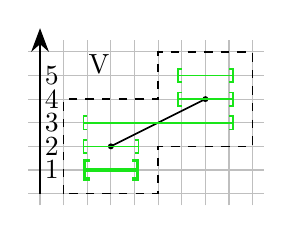
\begin{tikzpicture}[scale=0.6]
                \draw[step=0.5,lightgray,thin,xshift=-1cm,yshift=-1cm] (-0.75,-0.25) grid (4.25,3.25);
                \draw[-{Stealth[length=3mm]}=black] (-1.5,-1) -- (-1.5,2.5);
                \foreach[count=\i] \y in {-0.5,0,...,1.5} {
                    \draw (0,0) node at (-1.25,\y) {\i};
                }
                \filldraw[black] (0,0) circle (0.05);
                \filldraw[black] (2,1) circle (0.05);
                \draw[semithick, black] (0,0) -- (2,1);
                \draw[semithick,dashed] (-1,-1) -- (-1,1) -- (1,1) -- (1,2) -- (3,2) -- (3,0) -- (1,0) --  (1,-1) -- (-1,-1);
                \draw[very thick,MyGreen, arrows = {Bracket[sharp]-Bracket[sharp]}] (-0.6,-0.5)--(0.6,-0.5);
                \draw[semithick,MyGreen, arrows = {Bracket[sharp]-Bracket[sharp]}] (-0.6,0)--(0.6,0);
                \draw[semithick,MyGreen, arrows = {Bracket[sharp]-Bracket[sharp]}] (-0.6,0.5)--(2.6,0.5);
                \draw[semithick,MyGreen, arrows = {Bracket[sharp]-Bracket[sharp]}] (1.4,1)--(2.6,1);
                \draw[semithick,MyGreen, arrows = {Bracket[sharp]-Bracket[sharp]}] (1.4,1.5)--(2.6,1.5);

                \draw (0,0) node at (-0.25,1.75) {V};
            \end{tikzpicture} \\
            \\ \\
            \multicolumn{2}{c}{
                \begin{tikzpicture}[scale=0.6]
                    \foreach \y in {10.5,11,...,12} {
                        \draw[thin, lightgray] (-1.25,\y) -- (11.25,\y);
                    }
%                    Xies
                    \draw (0,0) node at (-4,12) {$V_{1}$};
                    \draw (0,0) node at (-4,11.5) {$F_{1}$};
                    \draw (0,0) node at (-5,11) {$T_{1} = \text{Translations}(V_{1},F_{1})$};
                    \draw (0,0) node at (-4,10.5) {$R_1 = T_1$};

                    \draw[thick,MyGreen,arrows = {Bracket[sharp]-Bracket[sharp]}] (-0.6,12)--(0.6,12);
                    \draw[thick,gray,arrows = {Bracket[sharp]-Bracket[sharp]}] (-0.6,11.5)--(2.6,11.5);
                    \draw[thick,gray,arrows = {Bracket[sharp]-Bracket[sharp]}] (4.4,11.5)--(10.6,11.5);
                    \draw[thick,violet,arrows = {Bracket[sharp]-Bracket[sharp]}] (-0.6,11)--(1.6,11);
                    \draw[thick,violet,arrows = {Bracket[sharp]-Bracket[sharp]}] (4.4,11)--(9.6,11);
                    \draw[thick,red,arrows = {Bracket[sharp]-Bracket[sharp]}] (-0.6,10.5)--(1.6,10.5);
                    \draw[thick,red,arrows = {Bracket[sharp]-Bracket[sharp]}] (4.4,10.5)--(9.6,10.5);
                    \filldraw[black] (-0.5,10.5) circle (0.05);
                    \filldraw[black] (0.5,10.5) circle (0.05);
                    \filldraw[black] (1.5,10.5) circle (0.05);
                    \filldraw[black] (4.5,10.5) circle (0.05);
                    \filldraw[black] (5.5,10.5) circle (0.05);
                    \filldraw[black] (6.5,10.5) circle (0.05);
                    \filldraw[black] (7.5,10.5) circle (0.05);
                    \filldraw[black] (8.5,10.5) circle (0.05);
                    \filldraw[black] (9.5,10.5) circle (0.05);

                \end{tikzpicture}}
        \end{tabular}
    \end{frame}
    \begin{frame}{Computing the visibility}
        \vspace{5em}
        \centering
        \hspace*{-2em}
        \begin{tabular}{c c}
            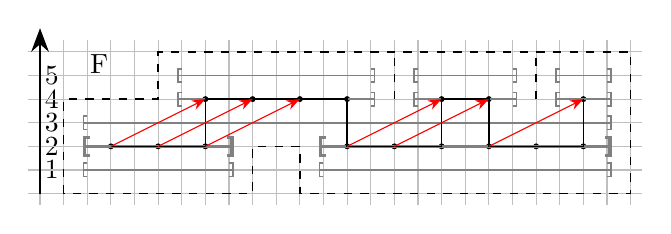
\begin{tikzpicture}[scale=0.6]
                \foreach[count=\i] \y in {-0.5,0,...,1.5} {
                    \draw (0,0) node at (-1.25,\y) {\i};
                }
                \draw[step=0.5,lightgray,thin,xshift=-1cm,yshift=-1cm] (-0.75,-0.25) grid (12.25,3.25);
                \draw[-{Stealth[length=3mm]}=black] (-1.5,-1) -- (-1.5,2.5);
                \filldraw[black] (0,0) circle (0.05);
                \filldraw[black] (1,0) circle (0.05);
                \filldraw[black] (2,0) circle (0.05);
                \filldraw[black] (2,1) circle (0.05);
                \filldraw[black] (3,1) circle (0.05);
                \filldraw[black] (4,1) circle (0.05);
                \filldraw[black] (5,1) circle (0.05);
                \filldraw[black] (5,0) circle (0.05);
                \filldraw[black] (6,0) circle (0.05);
                \filldraw[black] (7,0) circle (0.05);
                \filldraw[black] (7,1) circle (0.05);
                \filldraw[black] (8,1) circle (0.05);
                \filldraw[black] (8,0) circle (0.05);
                \filldraw[black] (9,0) circle (0.05);
                \filldraw[black] (10,0) circle (0.05);
                \filldraw[black] (10,1) circle (0.05);

                \draw[semithick,gray, arrows = {Bracket[sharp]-Bracket[sharp]}] (-0.6,-0.5)--(2.6,-0.5);
                \draw[semithick,gray, arrows = {Bracket[sharp]-Bracket[sharp]}] (4.4,-0.5)--(10.6,-0.5);
                \draw[very thick,gray, arrows = {Bracket[sharp]-Bracket[sharp]}] (-0.6,0)--(2.6,0);
                \draw[very thick,gray, arrows = {Bracket[sharp]-Bracket[sharp]}] (4.4,0)--(10.6,0);
                \draw[semithick,gray, arrows = {Bracket[sharp]-Bracket[sharp]}] (-0.6,0.5)--(10.6,0.5);
                \draw[semithick,gray, arrows = {Bracket[sharp]-Bracket[sharp]}] (1.4,1)--(5.6,1);
                \draw[semithick,gray, arrows = {Bracket[sharp]-Bracket[sharp]}] (6.4,1)--(8.6,1);
                \draw[semithick,gray, arrows = {Bracket[sharp]-Bracket[sharp]}] (9.4,1)--(10.6,1);
                \draw[semithick,gray, arrows = {Bracket[sharp]-Bracket[sharp]}] (1.4,1.5)--(5.6,1.5);
                \draw[semithick,gray, arrows = {Bracket[sharp]-Bracket[sharp]}] (6.4,1.5)--(8.6,1.5);
                \draw[semithick,gray, arrows = {Bracket[sharp]-Bracket[sharp]}] (9.4,1.5)--(10.6,1.5);

                \draw[semithick, black] (0,0) -- (2,0) -- (2,1) -- (5,1) -- (5,0) -- (7,0) -- (7,1) -- (8,1) -- (8,0) -- (10,0) -- (10,1);
                \draw[semithick,dashed] (6,1) -- (6,2);
                \draw[semithick,dashed] (9,1) -- (9,2);
                \draw[semithick,dashed] (-1,-1) -- (-1,1) -- (1,1) -- (1,2) -- (11,2) -- (11,-1) -- (4,-1) -- (4,0) -- (3,0) -- (3,-1) -- (-1,-1);

                \draw (0,0) node at (-0.25,1.75) {F};

                \draw[red,arrows = {-Stealth[]}] (0,0)--(2,1);
                \draw[red,arrows = {-Stealth[]}] (1,0)--(3,1);
                \draw[red,arrows = {-Stealth[]}] (2,0)--(4,1);
                \draw[red,arrows = {-Stealth[]}] (5,0)--(7,1);
                \draw[red,arrows = {-Stealth[]}] (6,0)--(8,1);
                \draw[red,arrows = {-Stealth[]}] (8,0)--(10,1);


            \end{tikzpicture} &
            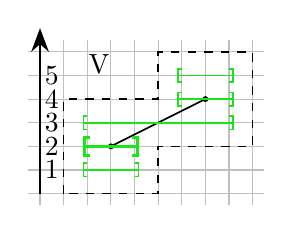
\begin{tikzpicture}[scale=0.6]
                \draw[step=0.5,lightgray,thin,xshift=-1cm,yshift=-1cm] (-0.75,-0.25) grid (4.25,3.25);
                \draw[-{Stealth[length=3mm]}=black] (-1.5,-1) -- (-1.5,2.5);
                \foreach[count=\i] \y in {-0.5,0,...,1.5} {
                    \draw (0,0) node at (-1.25,\y) {\i};
                }
                \filldraw[black] (0,0) circle (0.05);
                \filldraw[black] (2,1) circle (0.05);
                \draw[semithick, black] (0,0) -- (2,1);
                \draw[semithick,dashed] (-1,-1) -- (-1,1) -- (1,1) -- (1,2) -- (3,2) -- (3,0) -- (1,0) --  (1,-1) -- (-1,-1);

                \draw[semithick,MyGreen, arrows = {Bracket[sharp]-Bracket[sharp]}] (-0.6,-0.5)--(0.6,-0.5);
                \draw[very thick,MyGreen, arrows = {Bracket[sharp]-Bracket[sharp]}] (-0.6,0)--(0.6,0);
                \draw[semithick,MyGreen, arrows = {Bracket[sharp]-Bracket[sharp]}] (-0.6,0.5)--(2.6,0.5);
                \draw[semithick,MyGreen, arrows = {Bracket[sharp]-Bracket[sharp]}] (1.4,1)--(2.6,1);
                \draw[semithick,MyGreen, arrows = {Bracket[sharp]-Bracket[sharp]}] (1.4,1.5)--(2.6,1.5);

                \draw (0,0) node at (-0.25,1.75) {V};
            \end{tikzpicture} \\
            \\ \\
            \multicolumn{2}{c}{
                \begin{tikzpicture}[scale=0.6]
                    \foreach \y in {10.5,11,...,12} {
                        \draw[thin, lightgray] (-1.25,\y) -- (11.25,\y);
                    }
%                    Xies
                    \draw (0,0) node at (-4,12) {$V_2$};
                    \draw (0,0) node at (-4,11.5) {$F_2$};
                    \draw (0,0) node at (-4,11) {$T_2$};
                    \draw (0,0) node at (-4,10.5) {$R_2 = T_2 \cap R_1$};

                    \draw[thick,MyGreen,arrows = {Bracket[sharp]-Bracket[sharp]}] (-0.6,12)--(0.6,12);
                    \draw[thick,gray,arrows = {Bracket[sharp]-Bracket[sharp]}] (-0.6,11.5)--(2.6,11.5);
                    \draw[thick,gray,arrows = {Bracket[sharp]-Bracket[sharp]}] (4.4,11.5)--(10.6,11.5);
                    \draw[thick,violet,arrows = {Bracket[sharp]-Bracket[sharp]}] (-0.6,11)--(1.6,11);
                    \draw[thick,violet,arrows = {Bracket[sharp]-Bracket[sharp]}] (4.4,11)--(9.6,11);
                    \draw[thick,red,arrows = {Bracket[sharp]-Bracket[sharp]}] (-0.6,10.5)--(1.6,10.5);
                    \draw[thick,red,arrows = {Bracket[sharp]-Bracket[sharp]}] (4.4,10.5)--(9.6,10.5);
                    \filldraw[black] (-0.5,10.5) circle (0.05);
                    \filldraw[black] (0.5,10.5) circle (0.05);
                    \filldraw[black] (1.5,10.5) circle (0.05);
                    \filldraw[black] (4.5,10.5) circle (0.05);
                    \filldraw[black] (5.5,10.5) circle (0.05);
                    \filldraw[black] (6.5,10.5) circle (0.05);
                    \filldraw[black] (7.5,10.5) circle (0.05);
                    \filldraw[black] (8.5,10.5) circle (0.05);
                    \filldraw[black] (9.5,10.5) circle (0.05);

                \end{tikzpicture}}
        \end{tabular}
    \end{frame}
    \begin{frame}{Computing the visibility}
        \vspace{5em}
        \centering
        \hspace*{-2em}
        \begin{tabular}{c c}
            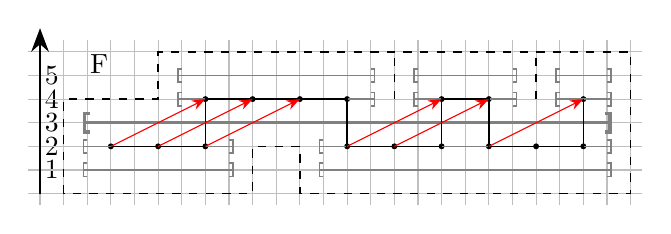
\begin{tikzpicture}[scale=0.6]
                \foreach[count=\i] \y in {-0.5,0,...,1.5} {
                    \draw (0,0) node at (-1.25,\y) {\i};
                }
                \draw[step=0.5,lightgray,thin,xshift=-1cm,yshift=-1cm] (-0.75,-0.25) grid (12.25,3.25);
                \draw[-{Stealth[length=3mm]}=black] (-1.5,-1) -- (-1.5,2.5);
                \filldraw[black] (0,0) circle (0.05);
                \filldraw[black] (1,0) circle (0.05);
                \filldraw[black] (2,0) circle (0.05);
                \filldraw[black] (2,1) circle (0.05);
                \filldraw[black] (3,1) circle (0.05);
                \filldraw[black] (4,1) circle (0.05);
                \filldraw[black] (5,1) circle (0.05);
                \filldraw[black] (5,0) circle (0.05);
                \filldraw[black] (6,0) circle (0.05);
                \filldraw[black] (7,0) circle (0.05);
                \filldraw[black] (7,1) circle (0.05);
                \filldraw[black] (8,1) circle (0.05);
                \filldraw[black] (8,0) circle (0.05);
                \filldraw[black] (9,0) circle (0.05);
                \filldraw[black] (10,0) circle (0.05);
                \filldraw[black] (10,1) circle (0.05);

                \draw[semithick,gray, arrows = {Bracket[sharp]-Bracket[sharp]}] (-0.6,-0.5)--(2.6,-0.5);
                \draw[semithick,gray, arrows = {Bracket[sharp]-Bracket[sharp]}] (4.4,-0.5)--(10.6,-0.5);
                \draw[semithick,gray, arrows = {Bracket[sharp]-Bracket[sharp]}] (-0.6,0)--(2.6,0);
                \draw[semithick,gray, arrows = {Bracket[sharp]-Bracket[sharp]}] (4.4,0)--(10.6,0);
                \draw[very thick,gray, arrows = {Bracket[sharp]-Bracket[sharp]}] (-0.6,0.5)--(10.6,0.5);
                \draw[semithick,gray, arrows = {Bracket[sharp]-Bracket[sharp]}] (1.4,1)--(5.6,1);
                \draw[semithick,gray, arrows = {Bracket[sharp]-Bracket[sharp]}] (6.4,1)--(8.6,1);
                \draw[semithick,gray, arrows = {Bracket[sharp]-Bracket[sharp]}] (9.4,1)--(10.6,1);
                \draw[semithick,gray, arrows = {Bracket[sharp]-Bracket[sharp]}] (1.4,1.5)--(5.6,1.5);
                \draw[semithick,gray, arrows = {Bracket[sharp]-Bracket[sharp]}] (6.4,1.5)--(8.6,1.5);
                \draw[semithick,gray, arrows = {Bracket[sharp]-Bracket[sharp]}] (9.4,1.5)--(10.6,1.5);

                \draw[semithick, black] (0,0) -- (2,0) -- (2,1) -- (5,1) -- (5,0) -- (7,0) -- (7,1) -- (8,1) -- (8,0) -- (10,0) -- (10,1);
                \draw[semithick,dashed] (6,1) -- (6,2);
                \draw[semithick,dashed] (9,1) -- (9,2);
                \draw[semithick,dashed] (-1,-1) -- (-1,1) -- (1,1) -- (1,2) -- (11,2) -- (11,-1) -- (4,-1) -- (4,0) -- (3,0) -- (3,-1) -- (-1,-1);

                \draw (0,0) node at (-0.25,1.75) {F};

                \draw[red,arrows = {-Stealth[]}] (0,0)--(2,1);
                \draw[red,arrows = {-Stealth[]}] (1,0)--(3,1);
                \draw[red,arrows = {-Stealth[]}] (2,0)--(4,1);
                \draw[red,arrows = {-Stealth[]}] (5,0)--(7,1);
                \draw[red,arrows = {-Stealth[]}] (6,0)--(8,1);
                \draw[red,arrows = {-Stealth[]}] (8,0)--(10,1);


            \end{tikzpicture} &
            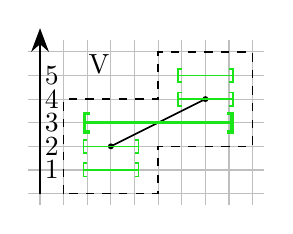
\begin{tikzpicture}[scale=0.6]
                \draw[step=0.5,lightgray,thin,xshift=-1cm,yshift=-1cm] (-0.75,-0.25) grid (4.25,3.25);
                \draw[-{Stealth[length=3mm]}=black] (-1.5,-1) -- (-1.5,2.5);
                \foreach[count=\i] \y in {-0.5,0,...,1.5} {
                    \draw (0,0) node at (-1.25,\y) {\i};
                }
                \filldraw[black] (0,0) circle (0.05);
                \filldraw[black] (2,1) circle (0.05);
                \draw[semithick, black] (0,0) -- (2,1);
                \draw[semithick,dashed] (-1,-1) -- (-1,1) -- (1,1) -- (1,2) -- (3,2) -- (3,0) -- (1,0) --  (1,-1) -- (-1,-1);

                \draw[semithick,MyGreen, arrows = {Bracket[sharp]-Bracket[sharp]}] (-0.6,-0.5)--(0.6,-0.5);
                \draw[semithick,MyGreen, arrows = {Bracket[sharp]-Bracket[sharp]}] (-0.6,0)--(0.6,0);
                \draw[very thick,MyGreen, arrows = {Bracket[sharp]-Bracket[sharp]}] (-0.6,0.5)--(2.6,0.5);
                \draw[semithick,MyGreen, arrows = {Bracket[sharp]-Bracket[sharp]}] (1.4,1)--(2.6,1);
                \draw[semithick,MyGreen, arrows = {Bracket[sharp]-Bracket[sharp]}] (1.4,1.5)--(2.6,1.5);

                \draw (0,0) node at (-0.25,1.75) {V};
            \end{tikzpicture} \\
            \\ \\
            \multicolumn{2}{c}{
                \begin{tikzpicture}[scale=0.6]
                    \foreach \y in {10.5,11,...,12} {
                        \draw[thin, lightgray] (-1.25,\y) -- (11.25,\y);
                    }
%                    Xies 3
                    \draw (0,0) node at (-4,12) {$V_3$};
                    \draw (0,0) node at (-4,11.5) {$F_3$};
                    \draw (0,0) node at (-4,11) {$T_3$};
                    \draw (0,0) node at (-4,10.5) {$R_3 = T_3 \cap R_2$};


                    \draw[thick,MyGreen,arrows = {Bracket[sharp]-Bracket[sharp]}] (-0.6,12)--(2.6,12);
                    \draw[thick,gray,arrows = {Bracket[sharp]-Bracket[sharp]}] (-0.6,11.5)--(10.6,11.5);
                    \draw[thick,violet,arrows = {Bracket[sharp]-Bracket[sharp]}] (-0.6,11)--(7.6,11);
                    \draw[thick,red,arrows = {Bracket[sharp]-Bracket[sharp]}] (-0.6,10.5)--(1.6,10.5);
                    \draw[thick,red,arrows = {Bracket[sharp]-Bracket[sharp]}] (4.4,10.5)--(7.6,10.5);
                    \filldraw[black] (-0.5,10.5) circle (0.05);
                    \filldraw[black] (0.5,10.5) circle (0.05);
                    \filldraw[black] (1.5,10.5) circle (0.05);
                    \filldraw[black] (4.5,10.5) circle (0.05);
                    \filldraw[black] (5.5,10.5) circle (0.05);
                    \filldraw[black] (6.5,10.5) circle (0.05);
                    \filldraw[black] (7.5,10.5) circle (0.05);

                \end{tikzpicture}}
        \end{tabular}
    \end{frame}
    \begin{frame}{Computing the visibility}
        \vspace{5em}
        \centering
        \hspace*{-2em}
        \begin{tabular}{c c}
            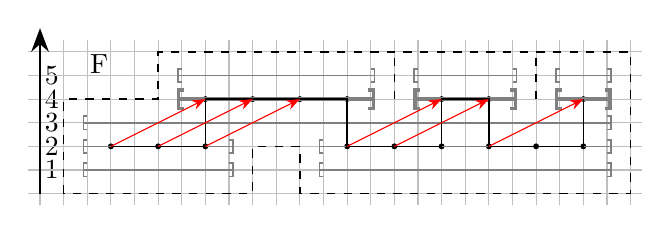
\begin{tikzpicture}[scale=0.6]
                \foreach[count=\i] \y in {-0.5,0,...,1.5} {
                    \draw (0,0) node at (-1.25,\y) {\i};
                }
                \draw[step=0.5,lightgray,thin,xshift=-1cm,yshift=-1cm] (-0.75,-0.25) grid (12.25,3.25);
                \draw[-{Stealth[length=3mm]}=black] (-1.5,-1) -- (-1.5,2.5);
                \filldraw[black] (0,0) circle (0.05);
                \filldraw[black] (1,0) circle (0.05);
                \filldraw[black] (2,0) circle (0.05);
                \filldraw[black] (2,1) circle (0.05);
                \filldraw[black] (3,1) circle (0.05);
                \filldraw[black] (4,1) circle (0.05);
                \filldraw[black] (5,1) circle (0.05);
                \filldraw[black] (5,0) circle (0.05);
                \filldraw[black] (6,0) circle (0.05);
                \filldraw[black] (7,0) circle (0.05);
                \filldraw[black] (7,1) circle (0.05);
                \filldraw[black] (8,1) circle (0.05);
                \filldraw[black] (8,0) circle (0.05);
                \filldraw[black] (9,0) circle (0.05);
                \filldraw[black] (10,0) circle (0.05);
                \filldraw[black] (10,1) circle (0.05);

                \draw[semithick,gray, arrows = {Bracket[sharp]-Bracket[sharp]}] (-0.6,-0.5)--(2.6,-0.5);
                \draw[semithick,gray, arrows = {Bracket[sharp]-Bracket[sharp]}] (4.4,-0.5)--(10.6,-0.5);
                \draw[semithick,gray, arrows = {Bracket[sharp]-Bracket[sharp]}] (-0.6,0)--(2.6,0);
                \draw[semithick,gray, arrows = {Bracket[sharp]-Bracket[sharp]}] (4.4,0)--(10.6,0);
                \draw[semithick,gray, arrows = {Bracket[sharp]-Bracket[sharp]}] (-0.6,0.5)--(10.6,0.5);
                \draw[very thick,gray, arrows = {Bracket[sharp]-Bracket[sharp]}] (1.4,1)--(5.6,1);
                \draw[very thick,gray, arrows = {Bracket[sharp]-Bracket[sharp]}] (6.4,1)--(8.6,1);
                \draw[very thick,gray, arrows = {Bracket[sharp]-Bracket[sharp]}] (9.4,1)--(10.6,1);
                \draw[semithick,gray, arrows = {Bracket[sharp]-Bracket[sharp]}] (1.4,1.5)--(5.6,1.5);
                \draw[semithick,gray, arrows = {Bracket[sharp]-Bracket[sharp]}] (6.4,1.5)--(8.6,1.5);
                \draw[semithick,gray, arrows = {Bracket[sharp]-Bracket[sharp]}] (9.4,1.5)--(10.6,1.5);

                \draw[semithick, black] (0,0) -- (2,0) -- (2,1) -- (5,1) -- (5,0) -- (7,0) -- (7,1) -- (8,1) -- (8,0) -- (10,0) -- (10,1);
                \draw[semithick,dashed] (6,1) -- (6,2);
                \draw[semithick,dashed] (9,1) -- (9,2);
                \draw[semithick,dashed] (-1,-1) -- (-1,1) -- (1,1) -- (1,2) -- (11,2) -- (11,-1) -- (4,-1) -- (4,0) -- (3,0) -- (3,-1) -- (-1,-1);

                \draw (0,0) node at (-0.25,1.75) {F};

                \draw[red,arrows = {-Stealth[]}] (0,0)--(2,1);
                \draw[red,arrows = {-Stealth[]}] (1,0)--(3,1);
                \draw[red,arrows = {-Stealth[]}] (2,0)--(4,1);
                \draw[red,arrows = {-Stealth[]}] (5,0)--(7,1);
                \draw[red,arrows = {-Stealth[]}] (6,0)--(8,1);
                \draw[red,arrows = {-Stealth[]}] (8,0)--(10,1);


            \end{tikzpicture} &
            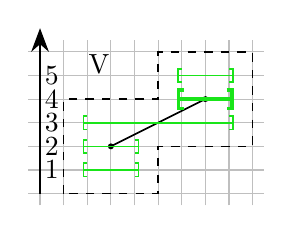
\begin{tikzpicture}[scale=0.6]
                \draw[step=0.5,lightgray,thin,xshift=-1cm,yshift=-1cm] (-0.75,-0.25) grid (4.25,3.25);
                \draw[-{Stealth[length=3mm]}=black] (-1.5,-1) -- (-1.5,2.5);
                \foreach[count=\i] \y in {-0.5,0,...,1.5} {
                    \draw (0,0) node at (-1.25,\y) {\i};
                }
                \filldraw[black] (0,0) circle (0.05);
                \filldraw[black] (2,1) circle (0.05);
                \draw[semithick, black] (0,0) -- (2,1);
                \draw[semithick,dashed] (-1,-1) -- (-1,1) -- (1,1) -- (1,2) -- (3,2) -- (3,0) -- (1,0) --  (1,-1) -- (-1,-1);

                \draw[semithick,MyGreen, arrows = {Bracket[sharp]-Bracket[sharp]}] (-0.6,-0.5)--(0.6,-0.5);
                \draw[semithick,MyGreen, arrows = {Bracket[sharp]-Bracket[sharp]}] (-0.6,0)--(0.6,0);
                \draw[semithick,MyGreen, arrows = {Bracket[sharp]-Bracket[sharp]}] (-0.6,0.5)--(2.6,0.5);
                \draw[very thick,MyGreen, arrows = {Bracket[sharp]-Bracket[sharp]}] (1.4,1)--(2.6,1);
                \draw[semithick,MyGreen, arrows = {Bracket[sharp]-Bracket[sharp]}] (1.4,1.5)--(2.6,1.5);

                \draw (0,0) node at (-0.25,1.75) {V};
            \end{tikzpicture} \\
            \\ \\
            \multicolumn{2}{c}{
                \begin{tikzpicture}[scale=0.6]
                    \foreach \y in {10.5,11,...,12} {
                        \draw[thin, lightgray] (-1.25,\y) -- (11.25,\y);
                    }
%                    Xies 4
                    \draw (0,0) node at (-4,12) {$V_4$};
                    \draw (0,0) node at (-4,11.5) {$F_4$};
                    \draw (0,0) node at (-4,11) {$T_4$};
                    \draw (0,0) node at (-4,10.5) {$R_4 = T_4 \cap R_3$};

                    \draw[thick,black,arrows = {-Stealth[]}] (-0.6,12)--(1.4,12);
                    \draw[thick,MyGreen,arrows = {Bracket[sharp]-Bracket[sharp]}] (1.4,12)--(2.6,12);
                    \draw[thick,gray,arrows = {Bracket[sharp]-Bracket[sharp]}] (1.4,11.5)--(5.6,11.5);
                    \draw[thick,gray,arrows = {Bracket[sharp]-Bracket[sharp]}] (6.4,11.5)--(8.6,11.5);
                    \draw[thick,gray,arrows = {Bracket[sharp]-Bracket[sharp]}] (9.4,11.5)--(10.6,11.5);
                    \draw[thick,violet,arrows = {Bracket[sharp]-Bracket[sharp]}] (-0.6,11)--(2.6,11);
                    \draw[thick,violet,arrows = {Bracket[sharp]-Bracket[sharp]}] (4.4,11)--(5.6,11);
                    \draw[thick,violet,arrows = {Bracket[sharp]-Bracket[sharp]}] (7.4,11)--(7.6,11);
                    \draw[thick,red,arrows = {Bracket[sharp]-Bracket[sharp]}] (-0.6,10.5)--(1.6,10.5);
                    \draw[thick,red,arrows = {Bracket[sharp]-Bracket[sharp]}] (4.4,10.5)--(5.6,10.5);
                    \draw[thick,red,arrows = {Bracket[sharp]-Bracket[sharp]}] (7.4,10.5)--(7.6,10.5);
                    \filldraw[black] (-0.5,10.5) circle (0.05);
                    \filldraw[black] (0.5,10.5) circle (0.05);
                    \filldraw[black] (1.5,10.5) circle (0.05);
                    \filldraw[black] (4.5,10.5) circle (0.05);
                    \filldraw[black] (5.5,10.5) circle (0.05);
                    \filldraw[black] (7.5,10.5) circle (0.05);


                \end{tikzpicture}}
        \end{tabular}
    \end{frame}
    \begin{frame}{Computing the visibility}
        \vspace{5em}
        \centering
        \hspace*{-2em}
        \begin{tabular}{c c}
            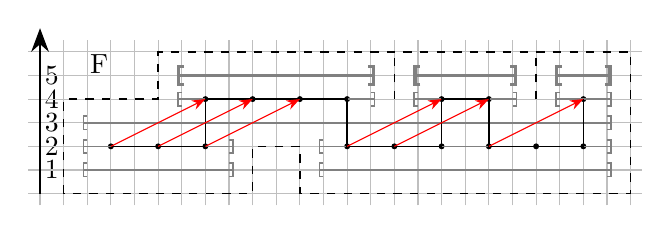
\begin{tikzpicture}[scale=0.6]
                \foreach[count=\i] \y in {-0.5,0,...,1.5} {
                    \draw (0,0) node at (-1.25,\y) {\i};
                }
                \draw[step=0.5,lightgray,thin,xshift=-1cm,yshift=-1cm] (-0.75,-0.25) grid (12.25,3.25);
                \draw[-{Stealth[length=3mm]}=black] (-1.5,-1) -- (-1.5,2.5);
                \filldraw[black] (0,0) circle (0.05);
                \filldraw[black] (1,0) circle (0.05);
                \filldraw[black] (2,0) circle (0.05);
                \filldraw[black] (2,1) circle (0.05);
                \filldraw[black] (3,1) circle (0.05);
                \filldraw[black] (4,1) circle (0.05);
                \filldraw[black] (5,1) circle (0.05);
                \filldraw[black] (5,0) circle (0.05);
                \filldraw[black] (6,0) circle (0.05);
                \filldraw[black] (7,0) circle (0.05);
                \filldraw[black] (7,1) circle (0.05);
                \filldraw[black] (8,1) circle (0.05);
                \filldraw[black] (8,0) circle (0.05);
                \filldraw[black] (9,0) circle (0.05);
                \filldraw[black] (10,0) circle (0.05);
                \filldraw[black] (10,1) circle (0.05);

                \draw[semithick,gray, arrows = {Bracket[sharp]-Bracket[sharp]}] (-0.6,-0.5)--(2.6,-0.5);
                \draw[semithick,gray, arrows = {Bracket[sharp]-Bracket[sharp]}] (4.4,-0.5)--(10.6,-0.5);
                \draw[semithick,gray, arrows = {Bracket[sharp]-Bracket[sharp]}] (-0.6,0)--(2.6,0);
                \draw[semithick,gray, arrows = {Bracket[sharp]-Bracket[sharp]}] (4.4,0)--(10.6,0);
                \draw[semithick,gray, arrows = {Bracket[sharp]-Bracket[sharp]}] (-0.6,0.5)--(10.6,0.5);
                \draw[semithick,gray, arrows = {Bracket[sharp]-Bracket[sharp]}] (1.4,1)--(5.6,1);
                \draw[semithick,gray, arrows = {Bracket[sharp]-Bracket[sharp]}] (6.4,1)--(8.6,1);
                \draw[semithick,gray, arrows = {Bracket[sharp]-Bracket[sharp]}] (9.4,1)--(10.6,1);
                \draw[very thick,gray, arrows = {Bracket[sharp]-Bracket[sharp]}] (1.4,1.5)--(5.6,1.5);
                \draw[very thick,gray, arrows = {Bracket[sharp]-Bracket[sharp]}] (6.4,1.5)--(8.6,1.5);
                \draw[very thick,gray, arrows = {Bracket[sharp]-Bracket[sharp]}] (9.4,1.5)--(10.6,1.5);

                \draw[semithick, black] (0,0) -- (2,0) -- (2,1) -- (5,1) -- (5,0) -- (7,0) -- (7,1) -- (8,1) -- (8,0) -- (10,0) -- (10,1);
                \draw[semithick,dashed] (6,1) -- (6,2);
                \draw[semithick,dashed] (9,1) -- (9,2);
                \draw[semithick,dashed] (-1,-1) -- (-1,1) -- (1,1) -- (1,2) -- (11,2) -- (11,-1) -- (4,-1) -- (4,0) -- (3,0) -- (3,-1) -- (-1,-1);

                \draw (0,0) node at (-0.25,1.75) {F};

                \draw[red,arrows = {-Stealth[]}] (0,0)--(2,1);
                \draw[red,arrows = {-Stealth[]}] (1,0)--(3,1);
                \draw[red,arrows = {-Stealth[]}] (2,0)--(4,1);
                \draw[red,arrows = {-Stealth[]}] (5,0)--(7,1);
                \draw[red,arrows = {-Stealth[]}] (6,0)--(8,1);
                \draw[red,arrows = {-Stealth[]}] (8,0)--(10,1);


            \end{tikzpicture} &
            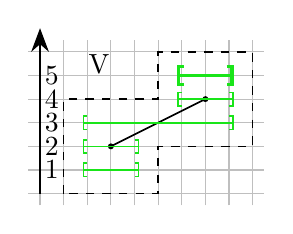
\begin{tikzpicture}[scale=0.6]
                \draw[step=0.5,lightgray,thin,xshift=-1cm,yshift=-1cm] (-0.75,-0.25) grid (4.25,3.25);
                \draw[-{Stealth[length=3mm]}=black] (-1.5,-1) -- (-1.5,2.5);
                \foreach[count=\i] \y in {-0.5,0,...,1.5} {
                    \draw (0,0) node at (-1.25,\y) {\i};
                }
                \filldraw[black] (0,0) circle (0.05);
                \filldraw[black] (2,1) circle (0.05);
                \draw[semithick, black] (0,0) -- (2,1);
                \draw[semithick,dashed] (-1,-1) -- (-1,1) -- (1,1) -- (1,2) -- (3,2) -- (3,0) -- (1,0) --  (1,-1) -- (-1,-1);

                \draw[semithick,MyGreen, arrows = {Bracket[sharp]-Bracket[sharp]}] (-0.6,-0.5)--(0.6,-0.5);
                \draw[semithick,MyGreen, arrows = {Bracket[sharp]-Bracket[sharp]}] (-0.6,0)--(0.6,0);
                \draw[semithick,MyGreen, arrows = {Bracket[sharp]-Bracket[sharp]}] (-0.6,0.5)--(2.6,0.5);
                \draw[semithick,MyGreen, arrows = {Bracket[sharp]-Bracket[sharp]}] (1.4,1)--(2.6,1);
                \draw[very thick,MyGreen, arrows = {Bracket[sharp]-Bracket[sharp]}] (1.4,1.5)--(2.6,1.5);

                \draw (0,0) node at (-0.25,1.75) {V};
            \end{tikzpicture} \\
            \\ \\
            \multicolumn{2}{c}{
                \begin{tikzpicture}[scale=0.6]
                    \foreach \y in {10.5,11,...,12} {
                        \draw[thin, lightgray] (-1.25,\y) -- (11.25,\y);
                    }
%                    Xies 5
                    \draw (0,0) node at (-4,12) {$V_5$};
                    \draw (0,0) node at (-4,11.5) {$F_5$};
                    \draw (0,0) node at (-4,11) {$T_5$};
                    \draw (0,0) node at (-4,10.5) {$R_5 = T_5 \cap R_4$};


                    \draw[thick,black,arrows = {-Stealth[]}] (-0.6,12)--(1.4,12);
                    \draw[thick,MyGreen,arrows = {Bracket[sharp]-Bracket[sharp]}] (1.4,12)--(2.6,12);
                    \draw[thick,gray,arrows = {Bracket[sharp]-Bracket[sharp]}] (1.4,11.5)--(5.6,11.5);
                    \draw[thick,gray,arrows = {Bracket[sharp]-Bracket[sharp]}] (6.4,11.5)--(8.6,11.5);
                    \draw[thick,gray,arrows = {Bracket[sharp]-Bracket[sharp]}] (9.4,11.5)--(10.6,11.5);
                    \draw[thick,violet,arrows = {Bracket[sharp]-Bracket[sharp]}] (-0.6,11)--(2.6,11);
                    \draw[thick,violet,arrows = {Bracket[sharp]-Bracket[sharp]}] (4.4,11)--(5.6,11);
                    \draw[thick,violet,arrows = {Bracket[sharp]-Bracket[sharp]}] (7.4,11)--(7.6,11);
                    \draw[thick,red,arrows = {Bracket[sharp]-Bracket[sharp]}] (-0.6,10.5)--(1.6,10.5);
                    \draw[thick,red,arrows = {Bracket[sharp]-Bracket[sharp]}] (4.4,10.5)--(5.6,10.5);
                    \draw[thick,red,arrows = {Bracket[sharp]-Bracket[sharp]}] (7.4,10.5)--(7.6,10.5);
                    \filldraw[black] (-0.5,10.5) circle (0.05);
                    \filldraw[black] (0.5,10.5) circle (0.05);
                    \filldraw[black] (1.5,10.5) circle (0.05);
                    \filldraw[black] (4.5,10.5) circle (0.05);
                    \filldraw[black] (5.5,10.5) circle (0.05);
                    \filldraw[black] (7.5,10.5) circle (0.05);

                \end{tikzpicture}}
        \end{tabular}
    \end{frame}

    \begin{frame}{Computing visibility : advantages}
        \begin{itemize}
            \item Simple data structure (arrays of intervals)
            \item Easy to implement \& parallelize -> GPU friendly
            \item Parameter-free
        \end{itemize}
    \end{frame}
    \begin{frame}{Computing visibility : advantages}
        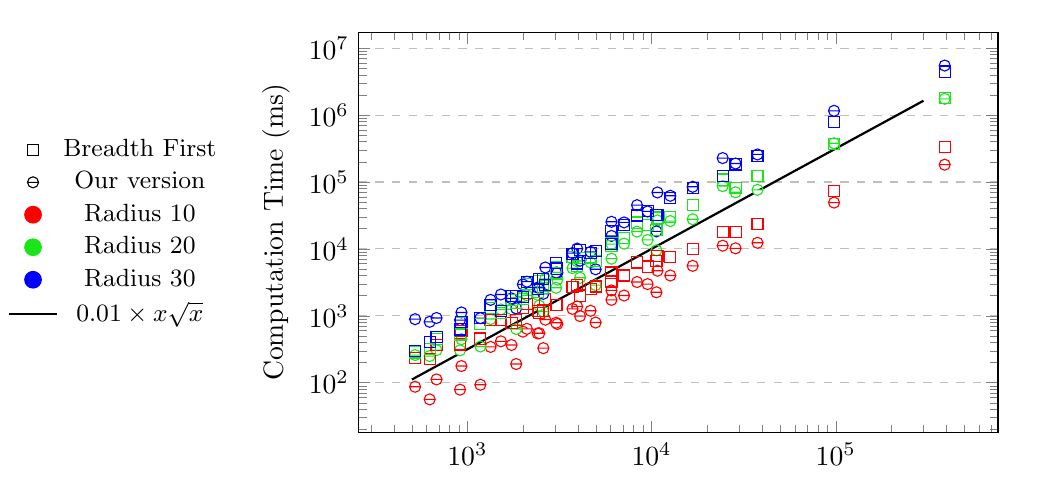
\begin{tikzpicture}
            \centering
            \hspace*{-1em}
            \begin{axis}[
                width=0.8\textwidth,
                height=0.55\textwidth,
                ylabel={Computation Time (ms)},
                ymajorgrids=true,
                grid style=dashed,
                ymode=log,
                xmode=log,
                xticklabel style={/pgf/number format/.cd,sci,precision=1},
                yticklabel style={/pgf/number format/.cd,sci,precision=1},
                legend style={
                    at={(-0.2,0.5)},
                    anchor=east,
                    draw=none,
                    fill=none,
                    font=\small
                },
            ]

                \addlegendimage{
                    black,
                    only marks,
                    mark=square,
                    mark options={solid}
                };
                \addlegendentry{Breadth First};
                \addlegendimage{
                    black,
                    only marks,
                    mark=halfcircle,
                    mark options={solid}
                };
                \addlegendentry{Our version}

                \addlegendimage{only marks, mark=*, color=red, mark size=3pt}
                \addlegendentry{Radius 10}
                \addlegendimage{only marks, mark=*, color=MyGreen, mark size=3pt}
                \addlegendentry{Radius 20}
                \addlegendimage{only marks, mark=*, color=blue, mark size=3pt}
                \addlegendentry{Radius 30}

                \addlegendimage{color=black,thick};
                \addlegendentry{$0.01\times x\sqrt{x}$}

                \addplot+[
                red,
                only marks,
                mark=halfcircle,
                mark options={solid}
                ] table[row sep=crcr] {
                    % torus
                    10624 2246.69\\
                    4968 793.426\\
                    2584 328.535\\
                    1840 190.401\\
                    1176 93.2502\\
                    912 78.7981\\
                    624 56.3769\\
                    % rcube
                    28568 10193.5\\
                    12632 4004.92\\
                    7088 2010.63\\
                    4664 1188.73\\
                    3080 755.754\\
                    2408 545.347\\
                    1736 366.541\\
                    % sphere9
                    24320 11169.1\\
                    10760 4720.44\\
                    6056 2397.79\\
                    3944 1380.38\\
                    2648 874.979\\
                    2000 580.0\\
                    1520 415.373\\
                    % leopold
                    8336 3196.55\\
                    3720 1268.46\\
                    2104 639.305\\
                    1336 342.873\\
                    928 177.54\\
                    680 112.142\\
                    520 87.0747\\
                    % goursat
                    37592 12335.6\\
                    16712 5582.38\\
                    9512 2976.21\\
                    6056 1731.32\\
                    4088 990.78\\
                    3032 788.507\\
                    2456 548.66\\
                    % d20
                    97844 49226.3\\
                    390235 181322\\
                };
                \addplot+[
                MyGreen,
                only marks,
                mark=halfcircle,
                mark options={solid}
                ] table[row sep=crcr] {
                    % torus
                    10624 9522.43\\
                    4968 2876.81\\
                    2584 1152.25\\
                    1840 635.332\\
                    1176 347.973\\
                    912 304.801\\
                    624 250.126\\
                    % rcube
                    28568 70137.9\\
                    12632 26063.0\\
                    7088 11985.8\\
                    4664 6239.51\\
                    3080 3468.31\\
                    2408 2059.84\\
                    1736 1254.2\\
                    % sphere9
                    24320 86616.9\\
                    10760 26605.7\\
                    6056 11813.5\\
                    3944 6516.92\\
                    2648 3564.03\\
                    2000 1949.32\\
                    1520 1244.89\\
                    % leopold
                    8336 18125.5\\
                    3720 5157.11\\
                    2104 2029.09\\
                    1336 896.186\\
                    928 446.136\\
                    680 306.651\\
                    520 259.078\\
                    % goursat
                    37592 76316.3\\
                    16712 27747.3\\
                    9512 13608.6\\
                    6056 7140.03\\
                    4088 3704.52\\
                    3032 2624.2\\
                    2456 1422.6\\
                    % d20
                    97844 378906\\
                    390235 1747780\\
                };
                \addplot+[
                blue,
                only marks,
                mark=halfcircle,
                mark options={solid}
                ] table[row sep=crcr] {
                    % torus
                    10624 18283.5\\
                    4968 4957.93\\
                    2584 2133.36\\
                    1840 1292.53\\
                    1176 922.51\\
                    912 863.731\\
                    624 813.638\\
                    % rcube
                    28568 188784.0\\
                    12632 62237.1\\
                    7088 24874.9\\
                    4664 9043.39\\
                    3080 4407.09\\
                    2408 2641.04\\
                    1736 1820.31\\
                    % sphere9
                    24320 227432.0\\
                    10760 69706.8\\
                    6056 25408.9\\
                    3944 10094.7\\
                    2648 5269.56\\
                    2000 2948.16\\
                    1520 2082.02\\
                    % leopold
                    8336 45045.4\\
                    3720 8638.42\\
                    2104 3238.48\\
                    1336 1731.9\\
                    928 1122.69\\
                    680 928.084\\
                    520 890.592\\
                    % goursat
                    37592 257981.0\\
                    16712 84729.7\\
                    9512 36298.8\\
                    6056 15640.2\\
                    4088 6662.17\\
                    3032 4431.71\\
                    2456 2621.98\\
                    % d20
                    97844 1157400\\
                    390235 5493200\\
                };
                \addplot+[
                red,
                only marks,
                mark=square,
                mark options={solid}
                ] table[row sep=crcr] {
                    % torus
                    10624 6658.15\\
                    4968 2740.74\\
                    2584 1198.02\\
                    1840 853.906\\
                    1176 456.784\\
                    912 373.028\\
                    624 229.479\\
                    % rcube
                    28568 17837.4\\
                    12632 7512.6\\
                    7088 4005.5\\
                    4664 2522.87\\
                    3080 1458.22\\
                    2408 1164.01\\
                    1736 770.449\\
                    % sphere9
                    24320 17922.8\\
                    10760 7845.85\\
                    6056 4431.68\\
                    3944 2840.96\\
                    2648 1774.39\\
                    2000 1292.66\\
                    1520 867.89\\
                    % leopold
                    8336 6268.17\\
                    3720 2697.19\\
                    2104 1489.4\\
                    1336 871.987\\
                    928 588.548\\
                    680 363.434\\
                    520 237.277\\
                    % goursat
                    37592 23416.9\\
                    16712 9923.63\\
                    9512 5446.57\\
                    6056 3256.35\\
                    4088 2008.14\\
                    3032 1467.76\\
                    2456 1107.06\\
                    % d20
                    97844 73606.0\\
                    390235 337851.0\\
                };
                \addplot+[
                MyGreen,
                only marks,
                mark=square,
                mark options={solid}
                ] table[row sep=crcr] {
                    % torus
                    10624 18932.3\\
                    4968 6555.12\\
                    2584 2621.4\\
                    1840 1571.18\\
                    1176 759.752\\
                    912 510.296\\
                    624 323.584\\
                    % rcube
                    28568 81041.4\\
                    12632 30169.2\\
                    7088 14369.6\\
                    4664 7318.29\\
                    3080 4377.33\\
                    2408 2255.89\\
                    1736 1743.95\\
                    % sphere9
                    24320 108696.0\\
                    10760 29433.6\\
                    6056 11092.9\\
                    3944 5535.89\\
                    2648 2759.14\\
                    2000 1770.88\\
                    1520 1103.44\\
                    % leopold
                    8336 24782.2\\
                    3720 7521.02\\
                    2104 2976.49\\
                    1336 1296.38\\
                    928 777.747\\
                    680 455.317\\
                    520 283.182\\
                    % goursat
                    37592 124066.0\\
                    16712 45347.2\\
                    9512 22445.1\\
                    6056 12308.8\\
                    4088 7370.63\\
                    3032 5317.86\\
                    2456 3356.28\\
                    % d20
                    97844 368339.0\\
                    390235 1784570.0\\
                };
                \addplot+[
                blue,
                only marks,
                mark=square,
                mark options={solid}
                ] table[row sep=crcr] {
                    % torus
                    10624 32025.4\\
                    4968 9426.13\\
                    2584 3596.87\\
                    1840 1975.03\\
                    1176 930.202\\
                    912 626.321\\
                    624 402.24\\
                    % rcube
                    28568 183072.0\\
                    12632 57696.6\\
                    7088 22998.7\\
                    4664 8654.47\\
                    3080 5090.0\\
                    2408 2538.87\\
                    1736 2004.77\\
                    % sphere9
                    24320 124004.0\\
                    10760 31699.4\\
                    6056 11704.3\\
                    3944 6068.31\\
                    2648 2885.91\\
                    2000 1888.12\\
                    1520 1170.45\\
                    % leopold
                    8336 31540.8\\
                    3720 8280.03\\
                    2104 3236.58\\
                    1336 1451.9\\
                    928 807.249\\
                    680 477.556\\
                    520 299.46\\
                    % goursat
                    37592 245584.0\\
                    16712 82093.2\\
                    9512 37091.0\\
                    6056 18530.7\\
                    4088 9711.66\\
                    3032 6214.95\\
                    2456 3523.63\\
                    % d20
                    97844 778491.0\\
                    390235 4409340.0\\
                };
                \addplot[
                    color=black,
                    thick,
                    domain=500:300000,
                    samples=200,
                ] {0.01*x^(1.5)};
            \end{axis}
        \end{tikzpicture}
    \end{frame}
    \begin{frame}{Computing visibility : advantages}
        \centering
        \hspace{1em}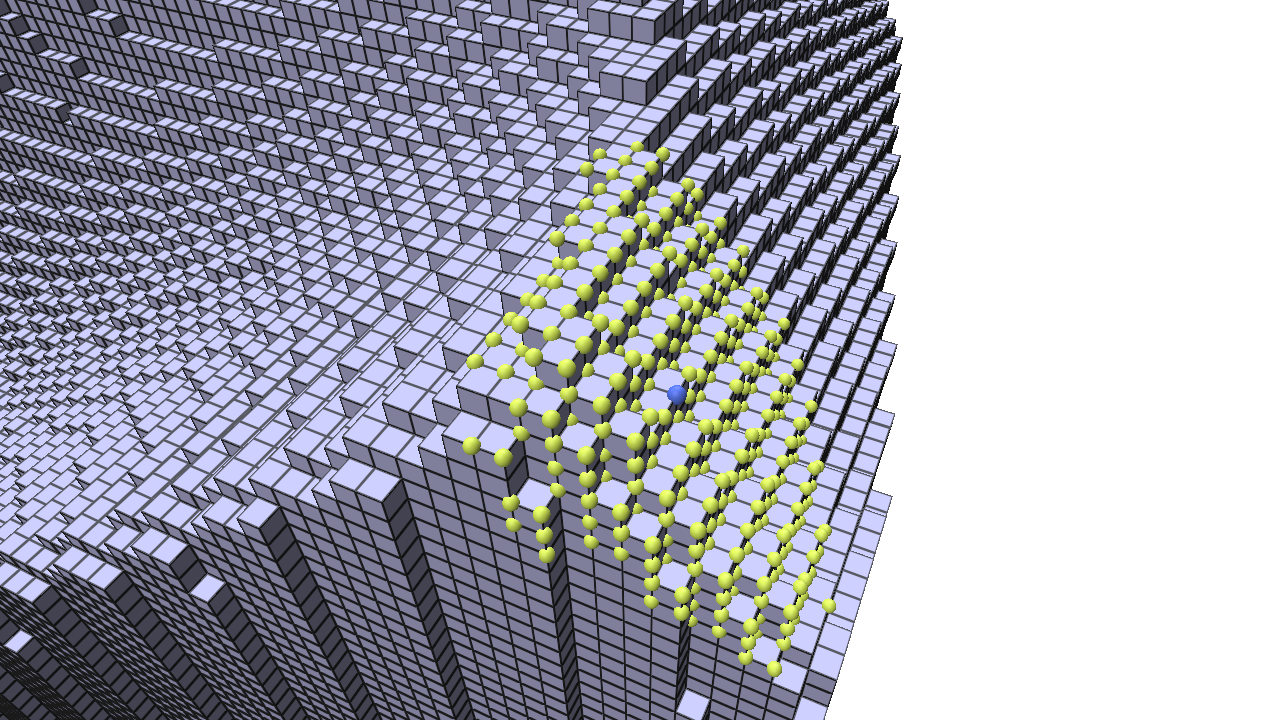
\includegraphics[width=0.7\textwidth,xshift=1em]{pictures/visibility_from_given_point_r_10}
        \newline
        \content{salliency aware visibility}
    \end{frame}
    \begin{frame}{Computing visibility : advantages}
        \centering
        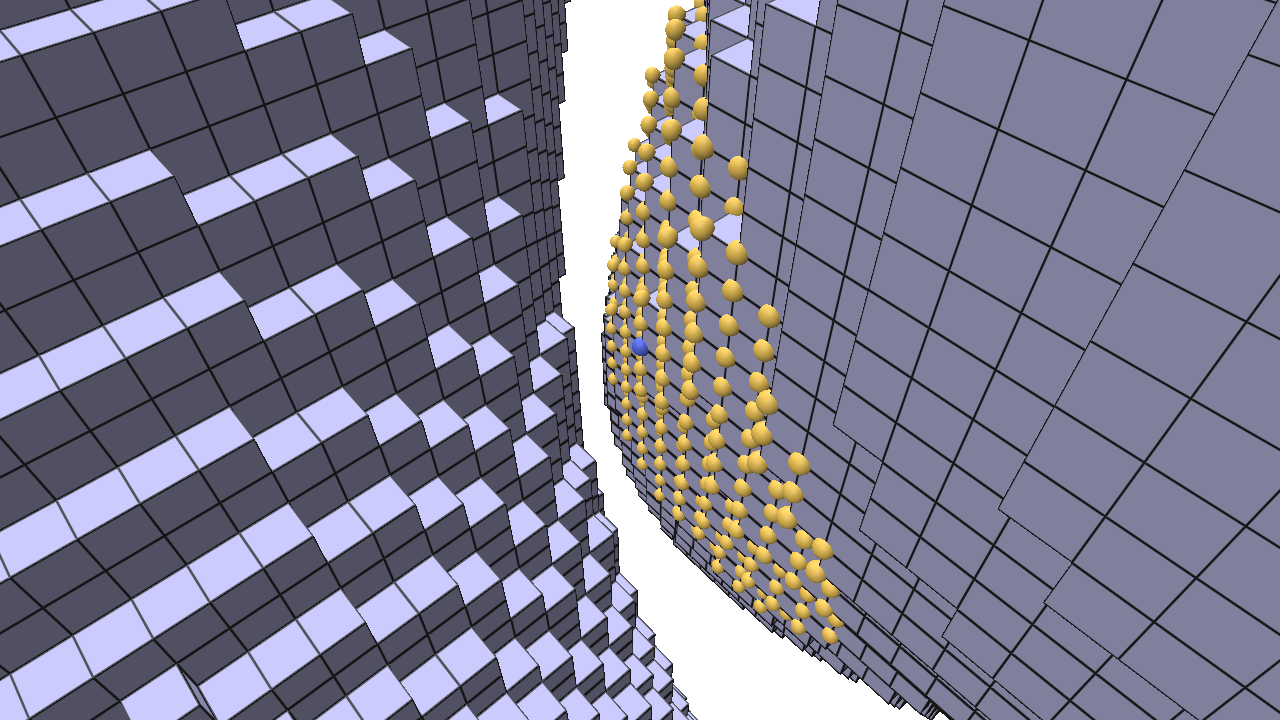
\includegraphics[width=0.7\textwidth]{pictures/visibility_aware_of_features}
        \newline
        \content{feature aware visibility}
    \end{frame}
    \begin{frame}{Computing visibility : recap}
        \begin{itemize}
            \item Simple data structure (arrays of intervals)
            \item Easy to implement \& parallelize -> GPU friendly
            \item Parameter-free
            \item Sequencial complexity of $\Theta \left(x \sqrt{x}\right)$ ($x$ : number of pointels)
            \item Is Salliency and Feature aware
        \end{itemize}
    \end{frame}


    \section{Normal \& curvature estimation}
    \begin{frame}{Covariance matrix estimation}
        \newcommand{\Kernel}[1]{\ensuremath{w_{\sigma}(#1)}}
        \begin{equation}
            \mathcal{V}_p = \sum_{q \in V_p} \Kernel{\|q-p\|}(q - c_p)(q - c_p)^T.
        \end{equation}
        \begin{itemize}
            \item $V_p$ : visible points from $p$
            \item $\Kernel{x}\coloneqq e^{-\frac{x^2}{2\sigma^2}}$ : weighting function
            \item $c_p = \frac{\sum_{q \in V_p} \Kernel{\|q-p\|} q}{\sum_{q \in V_p} \Kernel{\|q-p\|}}$ : weighted centroid of $V_p$
            \item Normal at $p$ is the eigenvector associated to the smallest eigenvalue of $\mathcal{V}_p$
            \item Orientation in the same direction as the average of the trivial normals to the surfels touching $p$
        \end{itemize}
    \end{frame}

    \begin{frame}{Normal estimation demo}
        \centering
        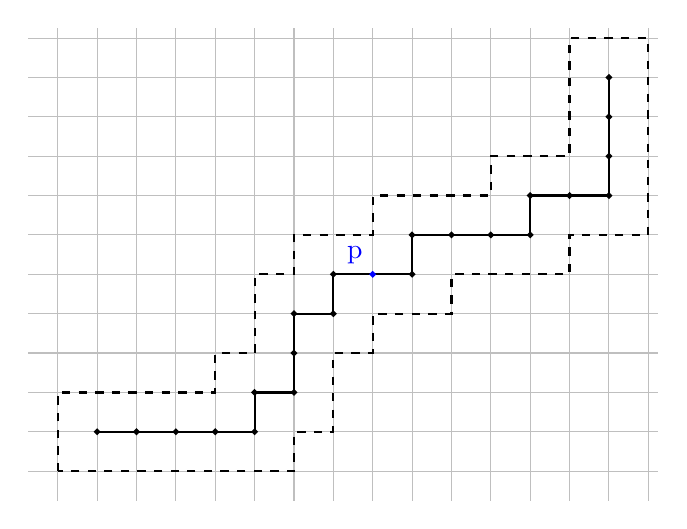
\begin{tikzpicture}[scale=0.5]
            \newcommand{\dpn}[3]{
                \filldraw[thick, #3] (#1,#2) circle (0.05)
            }
            \draw[step=1,lightgray,thin,xshift=-2cm,yshift=-2cm] (0.25,0.25) grid (16.25,12.25);
            \draw[thick] (0,0) -- (4,0) -- (4,1) -- (5,1) -- (5,3) -- (6,3) -- (6,4) -- (8,4) -- (8,5) -- (11,5) -- (11,6) -- (13,6) -- (13,9);
            \draw[thick,dashed] (-1,-1) -- (-1,1) -- (3,1) -- (3,2) -- (4,2) -- (4,4) -- (5,4) -- (5,5) -- (7,5) -- (7,6) -- (10,6) -- (10,7) -- (12,7) -- (12,10) -- (14,10) -- (14,5) -- (12,5) -- (12,4) -- (9,4) -- (9,3) -- (7,3) -- (7,2) -- (6,2) -- (6,0) -- (5,0) -- (5,-1) -- (-1,-1);

            \dpn{0}{0}{black};
            \dpn{1}{0}{black};
            \dpn{2}{0}{black};
            \dpn{3}{0}{black};
            \dpn{4}{0}{black};
            \dpn{4}{1}{black};
            \dpn{5}{1}{black};
            \dpn{5}{2}{black};
            \dpn{5}{3}{black};
            \dpn{6}{3}{black};
            \dpn{6}{4}{black};
            \dpn{7}{4}{blue} node[anchor=south east] {p};
            \dpn{8}{4}{black};
            \dpn{8}{5}{black};
            \dpn{9}{5}{black};
            \dpn{10}{5}{black};
            \dpn{11}{5}{black};
            \dpn{11}{6}{black};
            \dpn{12}{6}{black};
            \dpn{13}{6}{black};
            \dpn{13}{7}{black};
            \dpn{13}{8}{black};
            \dpn{13}{9}{black};
        \end{tikzpicture}
    \end{frame}
    \begin{frame}{Normal estimation demo}
        \centering
        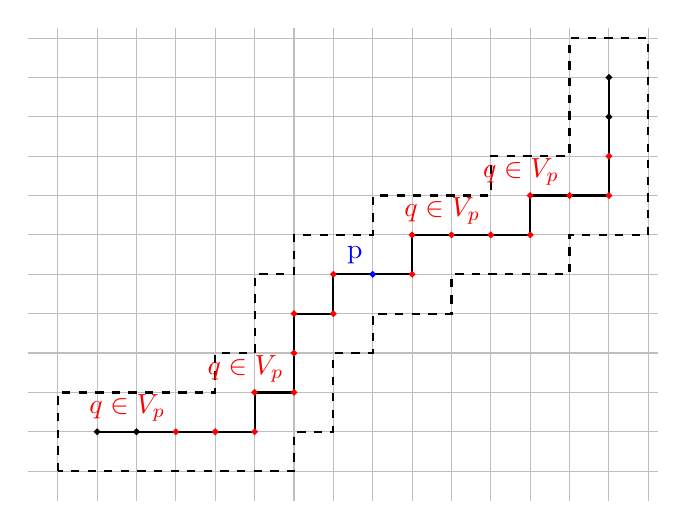
\begin{tikzpicture}[scale=0.5]
            \newcommand{\dpn}[3]{
                \filldraw[thick, #3] (#1,#2) circle (0.05)
            }
            \draw[step=1,lightgray,thin,xshift=-2cm,yshift=-2cm] (0.25,0.25) grid (16.25,12.25);
            \draw[thick] (0,0) -- (4,0) -- (4,1) -- (5,1) -- (5,3) -- (6,3) -- (6,4) -- (8,4) -- (8,5) -- (11,5) -- (11,6) -- (13,6) -- (13,9);
            \draw[thick,dashed] (-1,-1) -- (-1,1) -- (3,1) -- (3,2) -- (4,2) -- (4,4) -- (5,4) -- (5,5) -- (7,5) -- (7,6) -- (10,6) -- (10,7) -- (12,7) -- (12,10) -- (14,10) -- (14,5) -- (12,5) -- (12,4) -- (9,4) -- (9,3) -- (7,3) -- (7,2) -- (6,2) -- (6,0) -- (5,0) -- (5,-1) -- (-1,-1);

            \dpn{0}{0}{black};
            \dpn{1}{0}{black};
            \drawPoint{2}{0} node [anchor=south east] {$q \in V_p$};
            \drawPoint{3}{0};
            \drawPoint{4}{0};
            \drawPoint{4}{1};
            \drawPoint{5}{1} node [anchor=south east] {$q \in V_p$};
            \drawPoint{5}{2};
            \drawPoint{5}{3};
            \drawPoint{6}{3};
            \drawPoint{6}{4};
            \dpn{7}{4}{blue} node[anchor=south east] {p};
            \drawPoint{8}{4};
            \drawPoint{8}{5};
            \drawPoint{9}{5};
            \drawPoint{10}{5} node [anchor=south east] {$q \in V_p$};
            \drawPoint{11}{5};
            \drawPoint{11}{6};
            \drawPoint{12}{6} node [anchor=south east] {$q \in V_p$};
            \drawPoint{13}{6};
            \drawPoint{13}{7};
            \dpn{13}{8}{black};
            \dpn{13}{9}{black};
        \end{tikzpicture}
    \end{frame}
    \begin{frame}{Normal estimation demo}
        \centering
        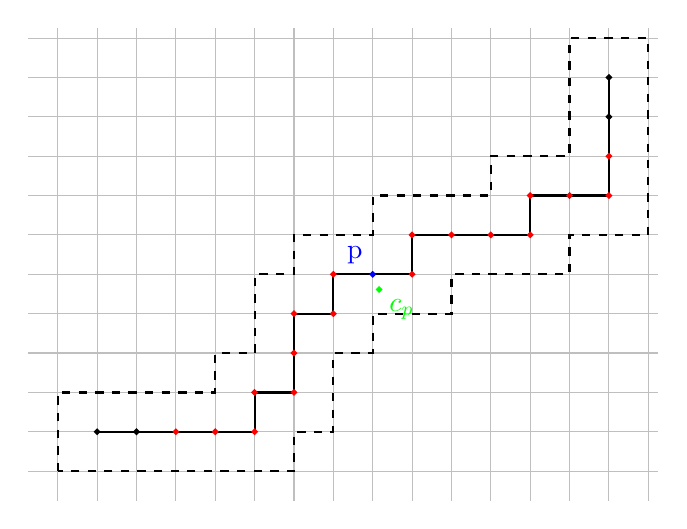
\begin{tikzpicture}[scale=0.5]
            \newcommand{\dpn}[3]{
                \filldraw[thick, #3] (#1,#2) circle (0.05)
            }
            \draw[step=1,lightgray,thin,xshift=-2cm,yshift=-2cm] (0.25,0.25) grid (16.25,12.25);
            \draw[thick] (0,0) -- (4,0) -- (4,1) -- (5,1) -- (5,3) -- (6,3) -- (6,4) -- (8,4) -- (8,5) -- (11,5) -- (11,6) -- (13,6) -- (13,9);
            \draw[thick,dashed] (-1,-1) -- (-1,1) -- (3,1) -- (3,2) -- (4,2) -- (4,4) -- (5,4) -- (5,5) -- (7,5) -- (7,6) -- (10,6) -- (10,7) -- (12,7) -- (12,10) -- (14,10) -- (14,5) -- (12,5) -- (12,4) -- (9,4) -- (9,3) -- (7,3) -- (7,2) -- (6,2) -- (6,0) -- (5,0) -- (5,-1) -- (-1,-1);

            \dpn{0}{0}{black};
            \dpn{1}{0}{black};
            \drawPoint{2}{0};
            \drawPoint{3}{0};
            \drawPoint{4}{0};
            \drawPoint{4}{1};
            \drawPoint{5}{1};
            \drawPoint{5}{2};
            \drawPoint{5}{3};
            \drawPoint{6}{3};
            \drawPoint{6}{4};
            \dpn{7}{4}{blue} node[anchor=south east] {p};
            \drawPoint{8}{4};
            \drawPoint{8}{5};
            \drawPoint{9}{5};
            \drawPoint{10}{5};
            \drawPoint{11}{5};
            \drawPoint{11}{6};
            \drawPoint{12}{6};
            \drawPoint{13}{6};
            \drawPoint{13}{7};
            \dpn{13}{8}{black};
            \dpn{13}{9}{black};

            \dpn{7.161978151947899}{3.6128706307461473}{green} node[anchor=north west] {$c_p$};

        \end{tikzpicture}
    \end{frame}
    \begin{frame}{Normal estimation demo}
        \centering
        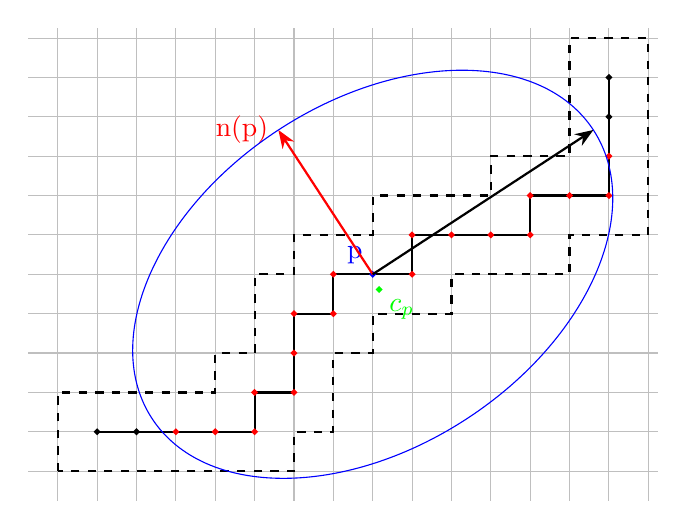
\begin{tikzpicture}[scale=0.5]
            \newcommand{\dpn}[3]{
                \filldraw[thick, #3] (#1,#2) circle (0.05)
            }
            \draw[step=1,lightgray,thin,xshift=-2cm,yshift=-2cm] (0.25,0.25) grid (16.25,12.25);
            \draw[thick] (0,0) -- (4,0) -- (4,1) -- (5,1) -- (5,3) -- (6,3) -- (6,4) -- (8,4) -- (8,5) -- (11,5) -- (11,6) -- (13,6) -- (13,9);
            \draw[thick,dashed] (-1,-1) -- (-1,1) -- (3,1) -- (3,2) -- (4,2) -- (4,4) -- (5,4) -- (5,5) -- (7,5) -- (7,6) -- (10,6) -- (10,7) -- (12,7) -- (12,10) -- (14,10) -- (14,5) -- (12,5) -- (12,4) -- (9,4) -- (9,3) -- (7,3) -- (7,2) -- (6,2) -- (6,0) -- (5,0) -- (5,-1) -- (-1,-1);

            \dpn{0}{0}{black};
            \dpn{1}{0}{black};
            \drawPoint{2}{0};
            \drawPoint{3}{0};
            \drawPoint{4}{0};
            \drawPoint{4}{1};
            \drawPoint{5}{1};
            \drawPoint{5}{2};
            \drawPoint{5}{3};
            \drawPoint{6}{3};
            \drawPoint{6}{4};
            \dpn{7}{4}{blue} node[anchor=south east] {p};
            \drawPoint{8}{4};
            \drawPoint{8}{5};
            \drawPoint{9}{5};
            \drawPoint{10}{5};
            \drawPoint{11}{5};
            \drawPoint{11}{6};
            \drawPoint{12}{6};
            \drawPoint{13}{6};
            \drawPoint{13}{7};
            \dpn{13}{8}{black};
            \dpn{13}{9}{black};

            \dpn{7.161978151947899}{3.6128706307461473}{green} node[anchor=north west] {$c_p$};

            \draw[thick, red, arrows=-Stealth] (7,4)--(7-2.3966844016072106,4+3.6651935054017417) node[anchor=east] {n(p)};
            \draw[thick, arrows=-Stealth] (7,4)--(7+5.60509486481847,4+3.6651935054017417);
            \draw[blue,thin,rotate around={33.18083015220524 :(7,4)}] (7,4) ellipse [x radius=6.697068901814696, y radius=4.379239608989947];
        \end{tikzpicture}
    \end{frame}

    \begin{frame}{Normal estimation : comparison}
        \centering
        \begin{tabular}{|c||c|c|}
            \hline
            Normals & With cube edges & Flat (no shading) \\
            \hline
            \hline
            \raisebox{18mm}{II} &
            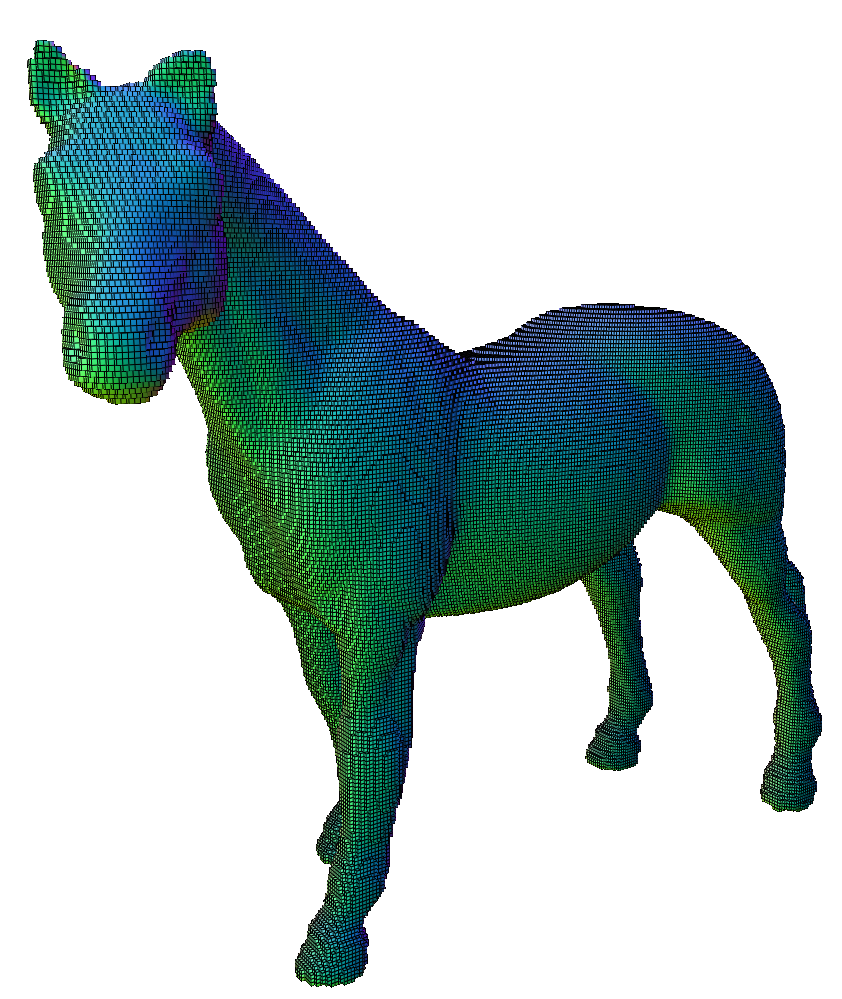
\includegraphics[width=0.28\textwidth]{pictures/horse_N_II_edge} &
            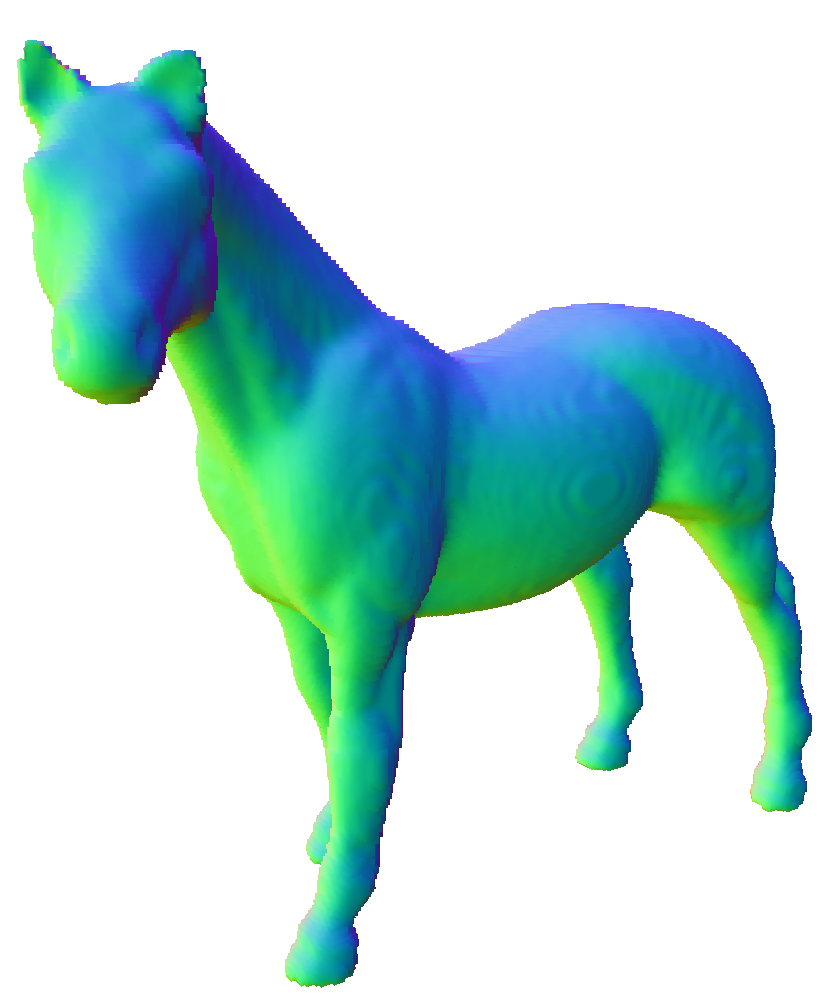
\includegraphics[width=0.28\textwidth]{pictures/horse_N_II_flat} \\
            %% 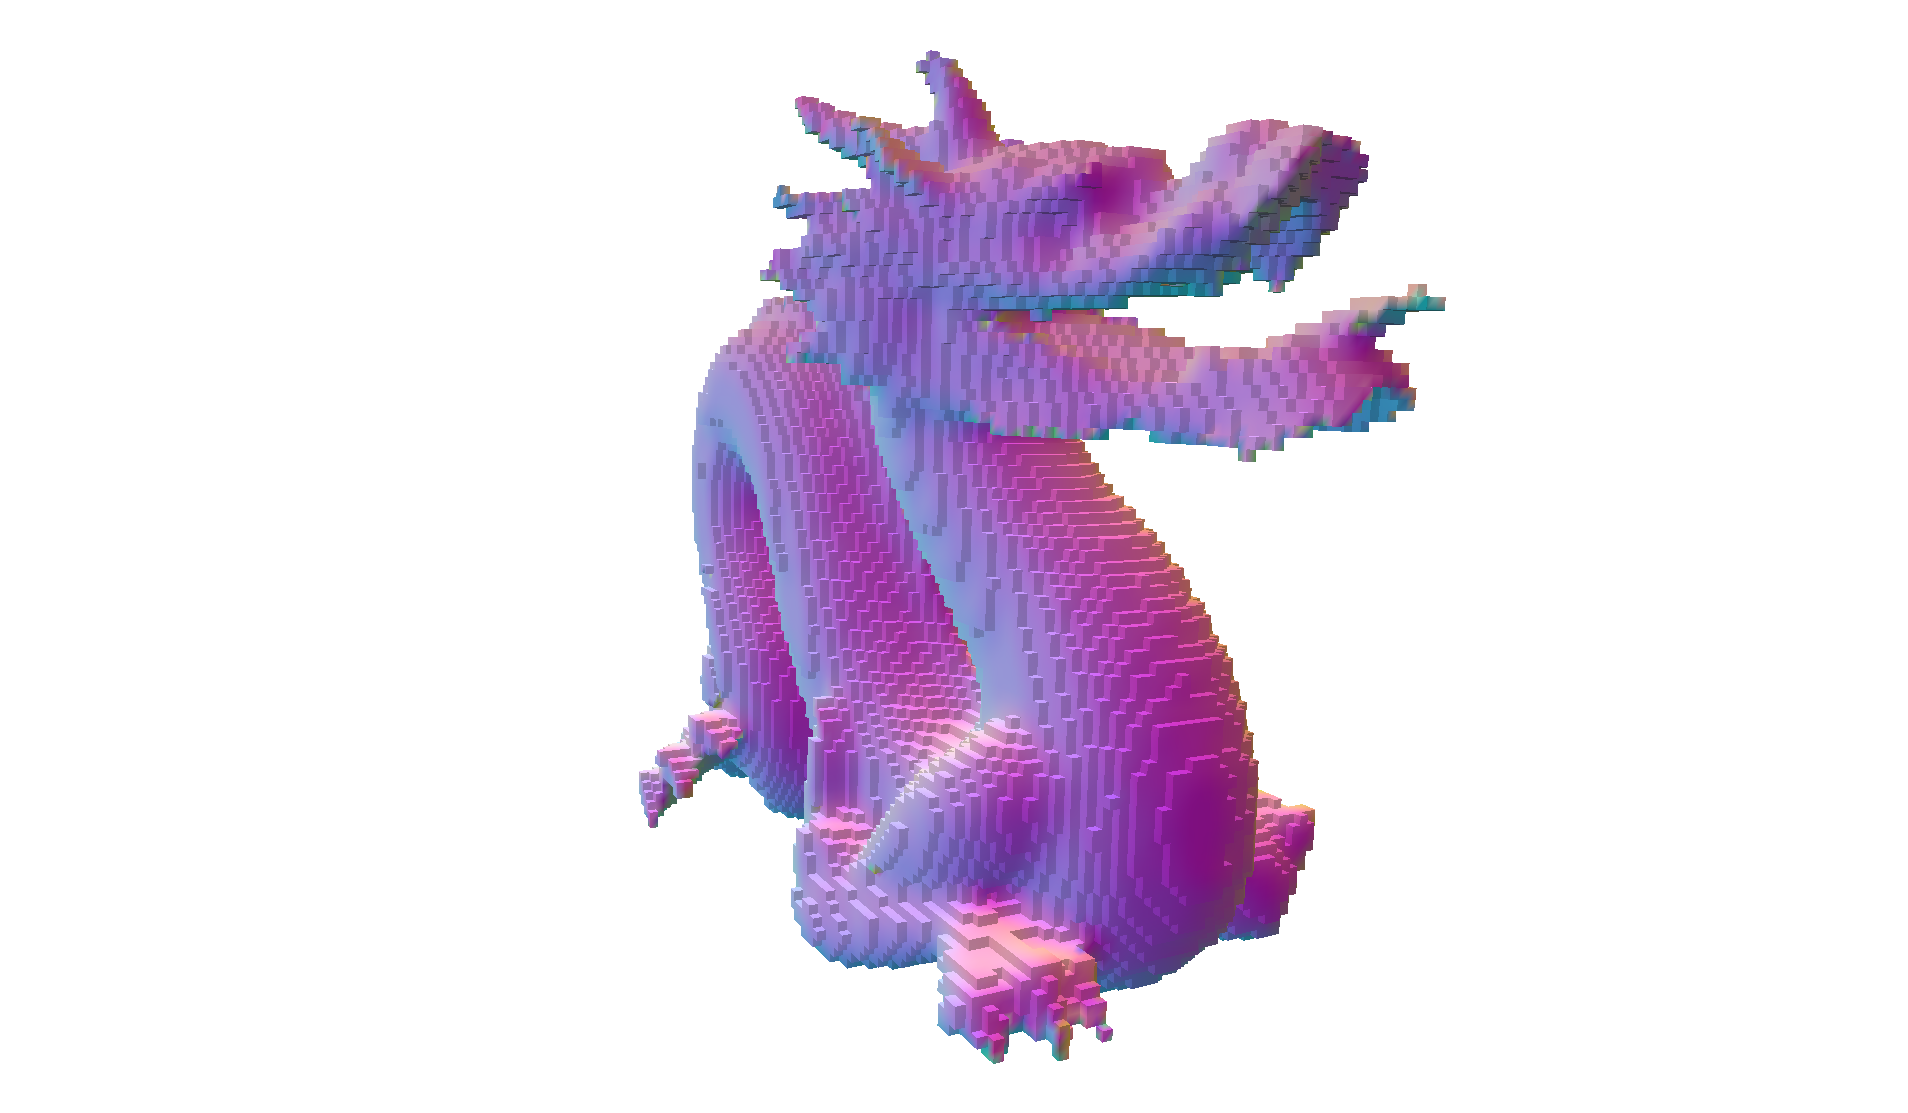
\includegraphics[width=0.4\textwidth]{pictures/chinese-dragon-normal-estimation-cubes-II} &
            %% 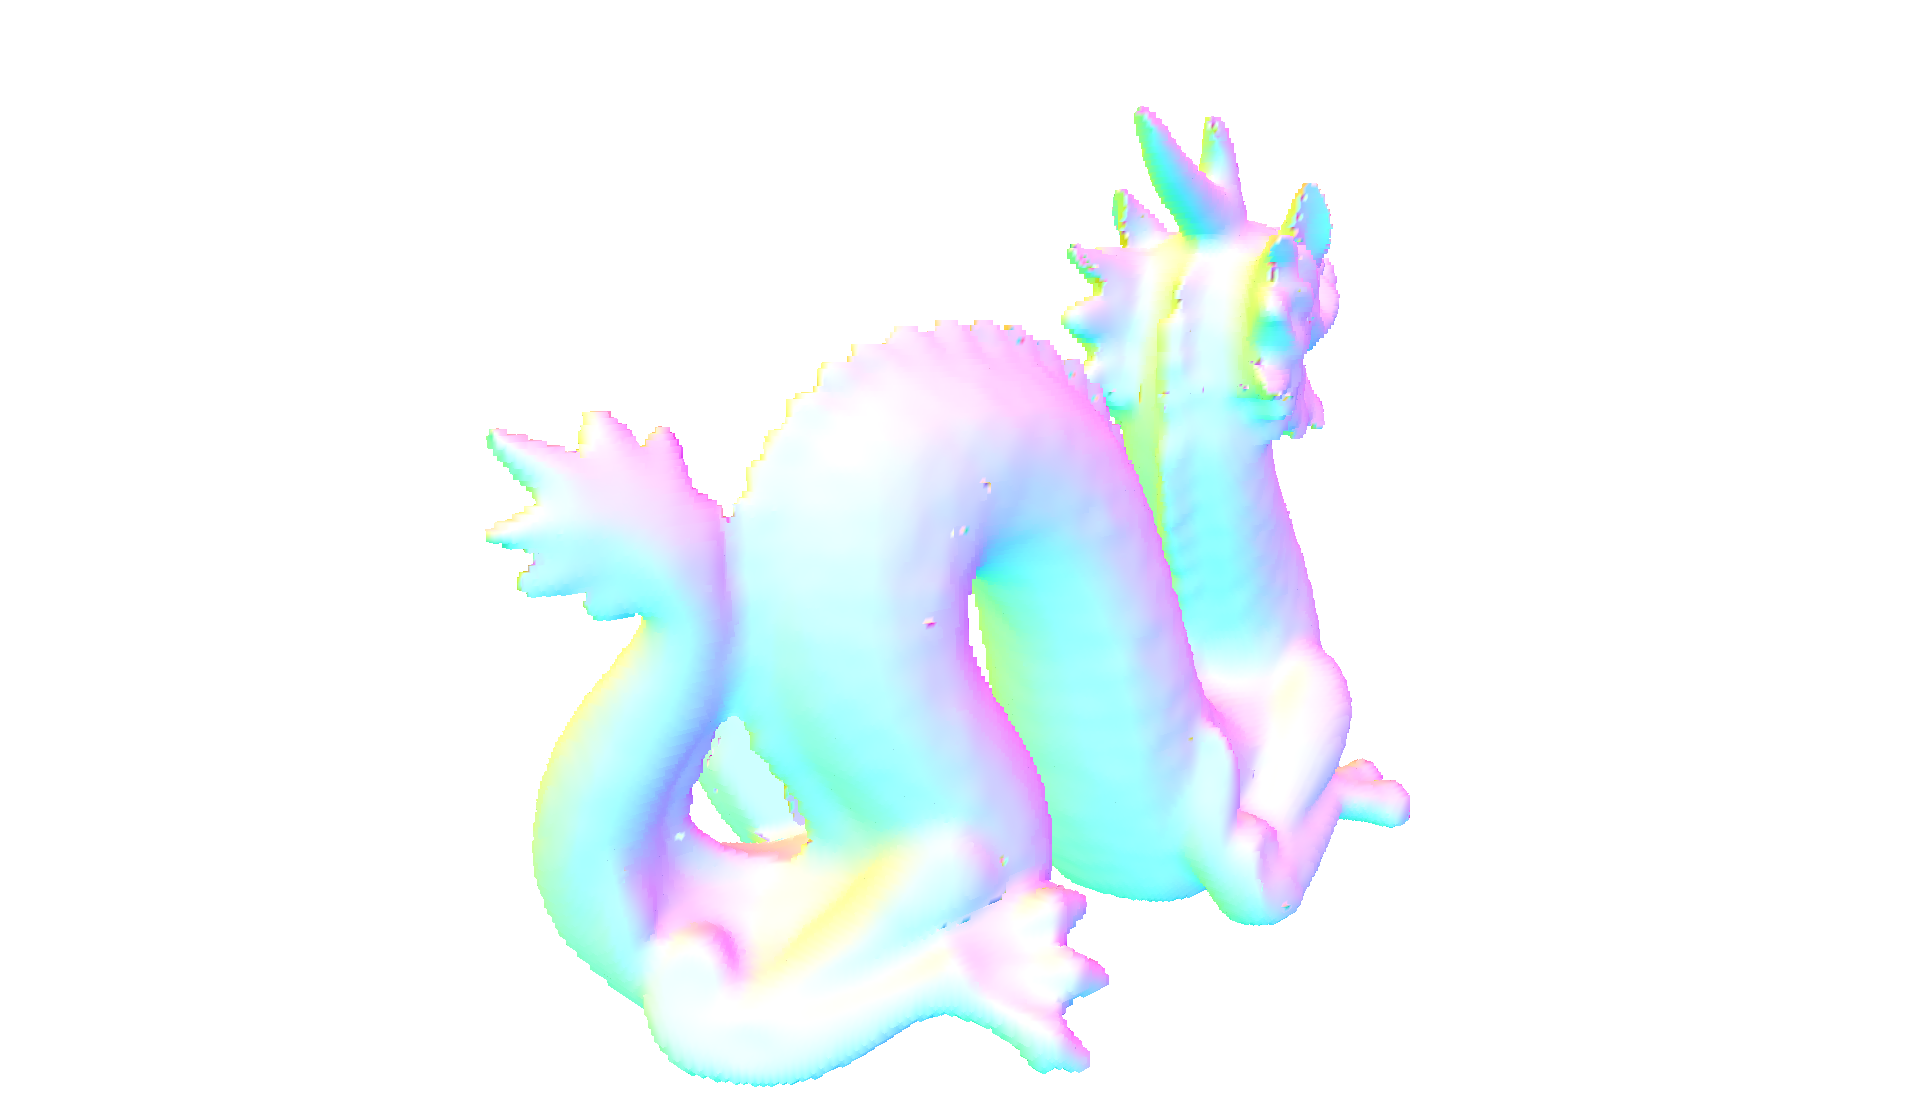
\includegraphics[width=0.4\textwidth]{pictures/chinese-dragon-normal-estimation-smooth-II} \\
            \hline
            \raisebox{18mm}{Ours} &
            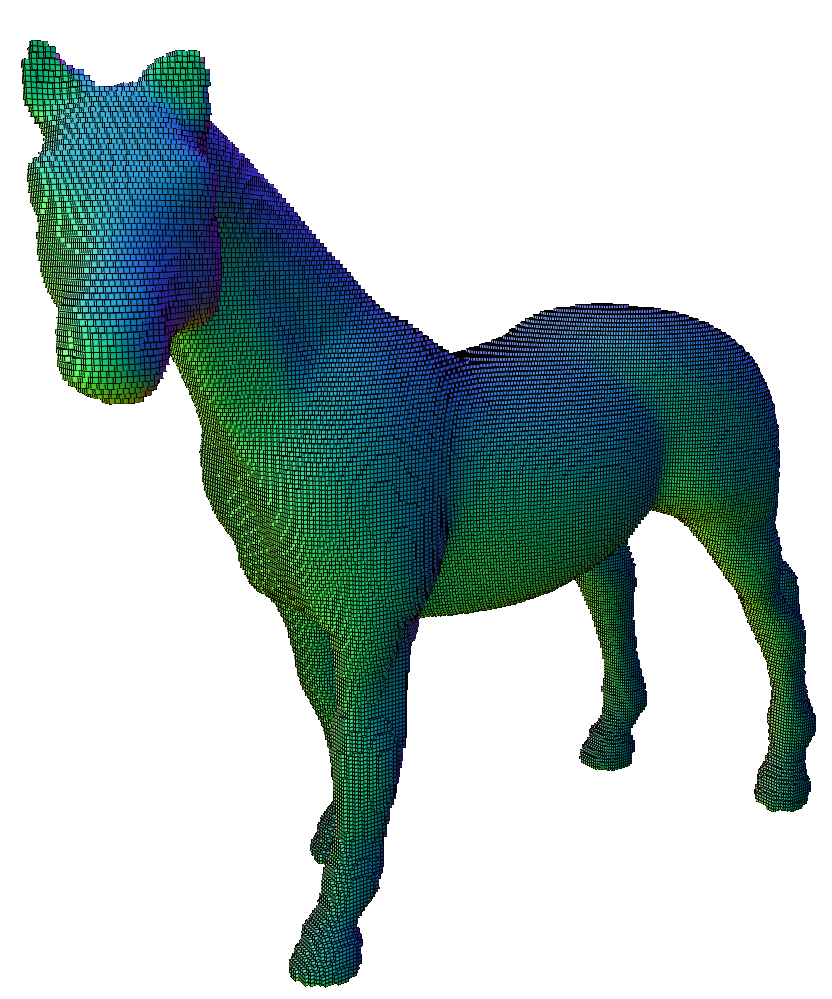
\includegraphics[width=0.28\textwidth]{pictures/horse_N_VN_edge} &
            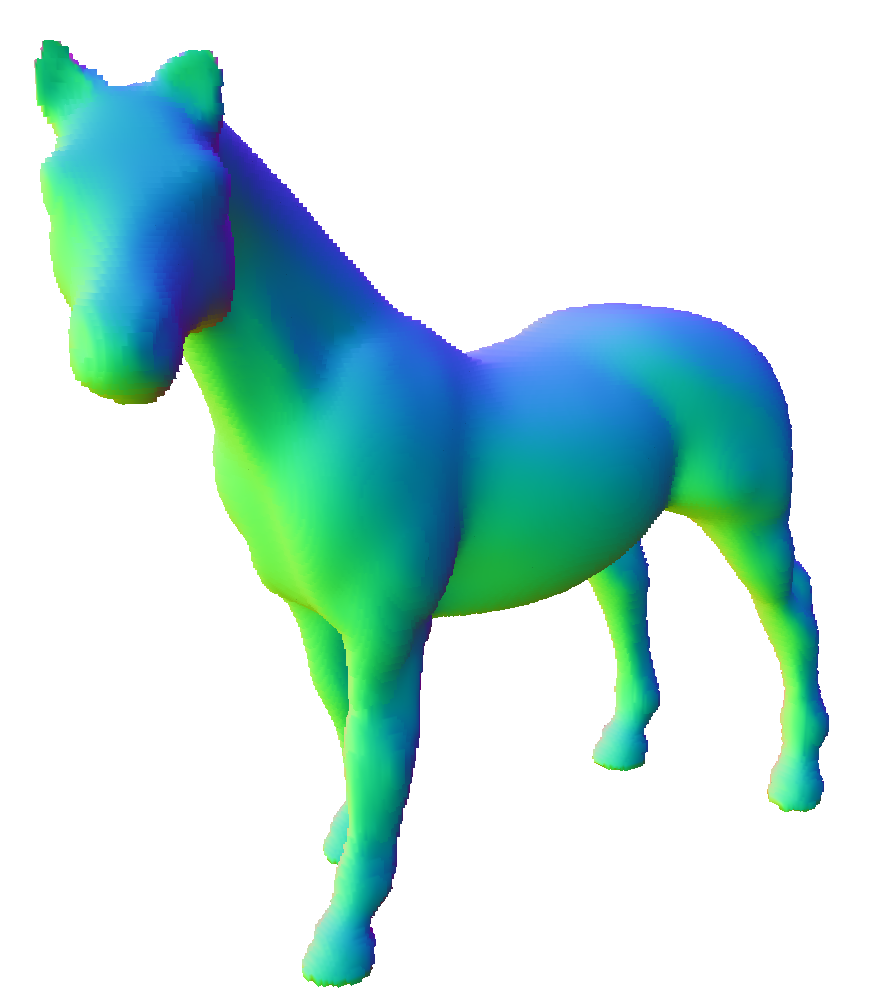
\includegraphics[width=0.28\textwidth]{pictures/horse_N_VN_flat} \\
            %% 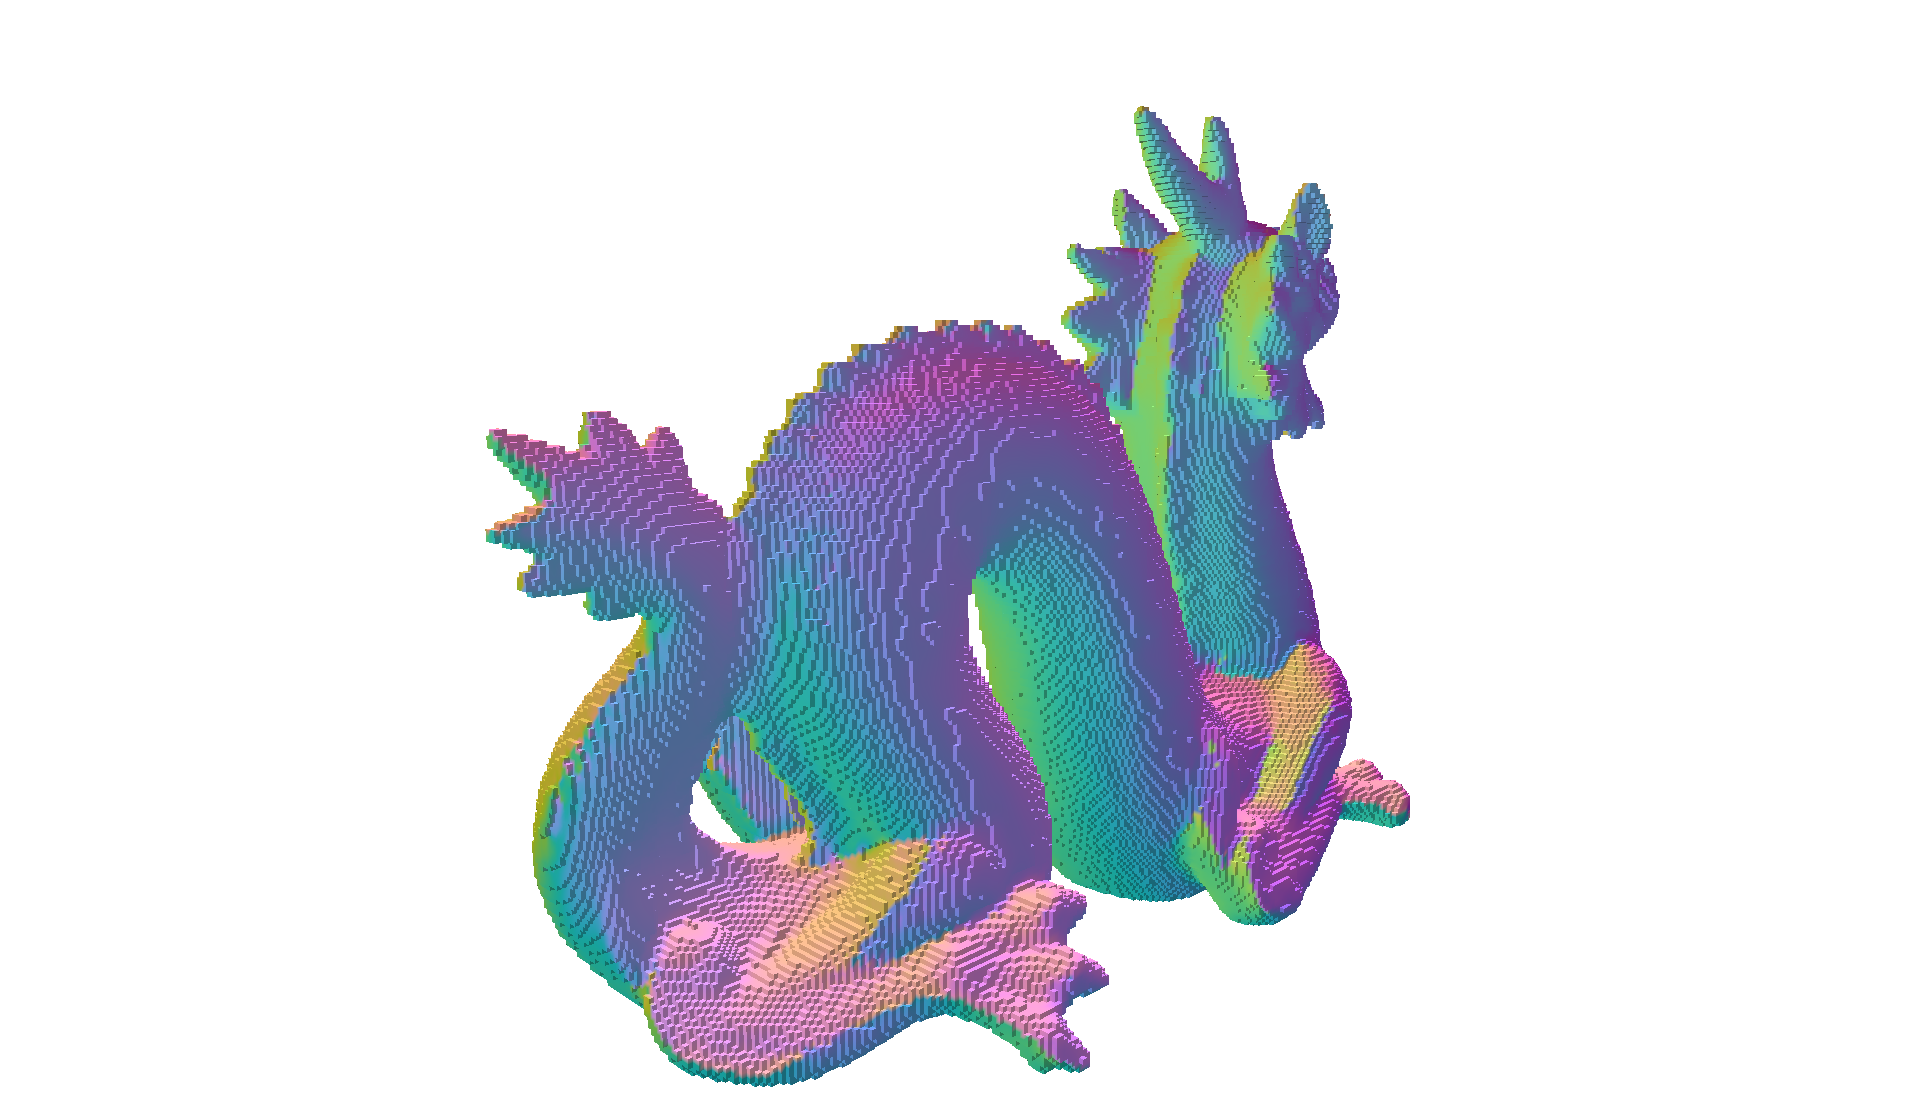
\includegraphics[width=0.4\textwidth]{pictures/chinese-dragon-normal-estimation-cubes-NV} &
            %% 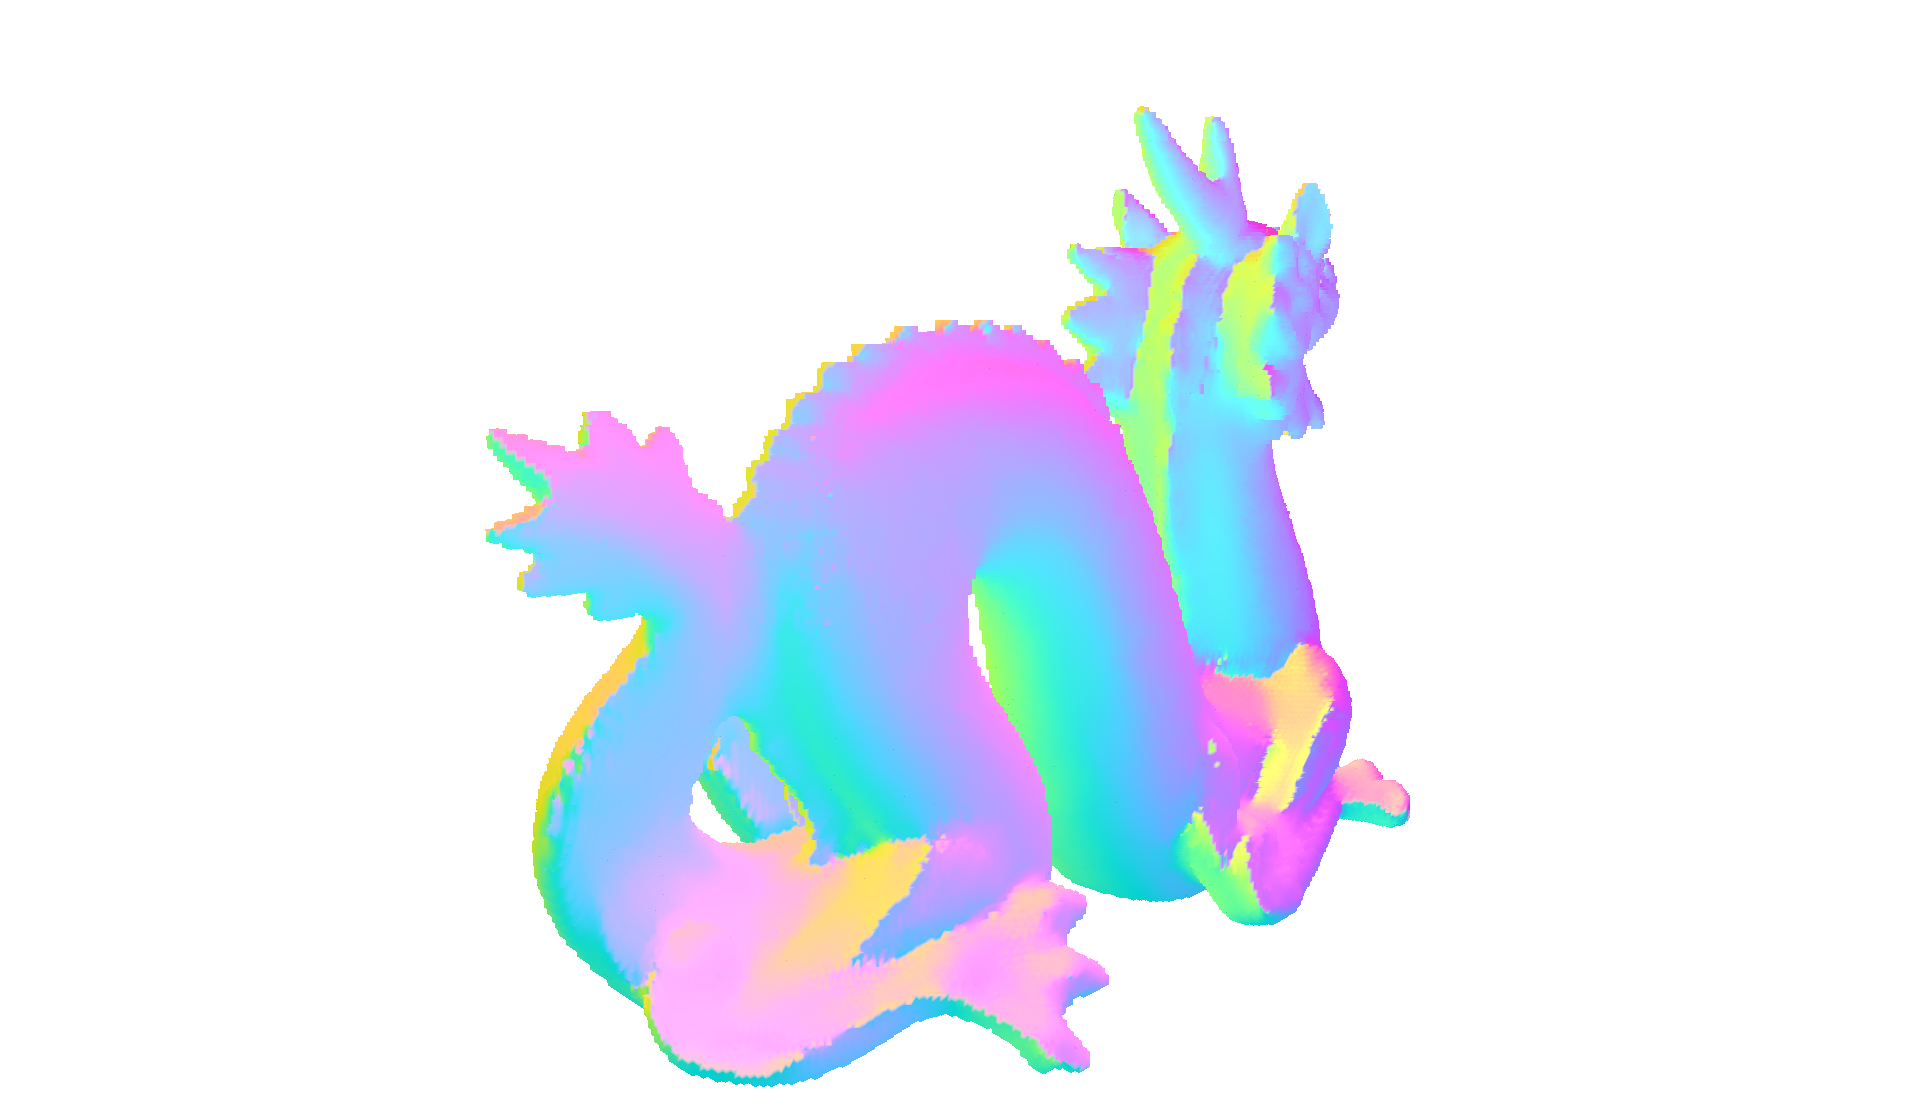
\includegraphics[width=0.4\textwidth]{pictures/chinese-dragon-normal-estimation-smooth-NV} \\
            \hline
        \end{tabular}
    \end{frame}
    \begin{frame}{Normal estimation : comparison}
        \centering
        \begin{tabular}{|c||c|c|}
            \hline
            Normals & With cube edges & Flat (no shading) \\
            \hline
            \hline
            \raisebox{9mm}{II} &
            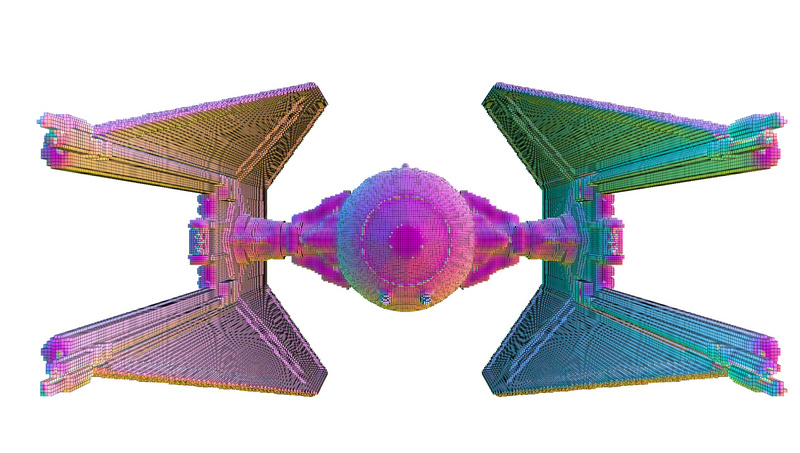
\includegraphics[width=0.33\textwidth]{pictures/tie256-IIN-flat-edge-small} &
            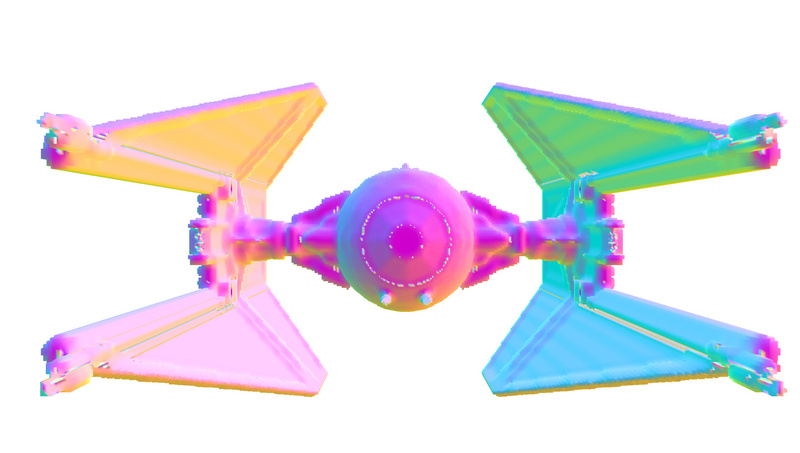
\includegraphics[width=0.33\textwidth]{pictures/tie256-IIN-flat-small} \\
            %% 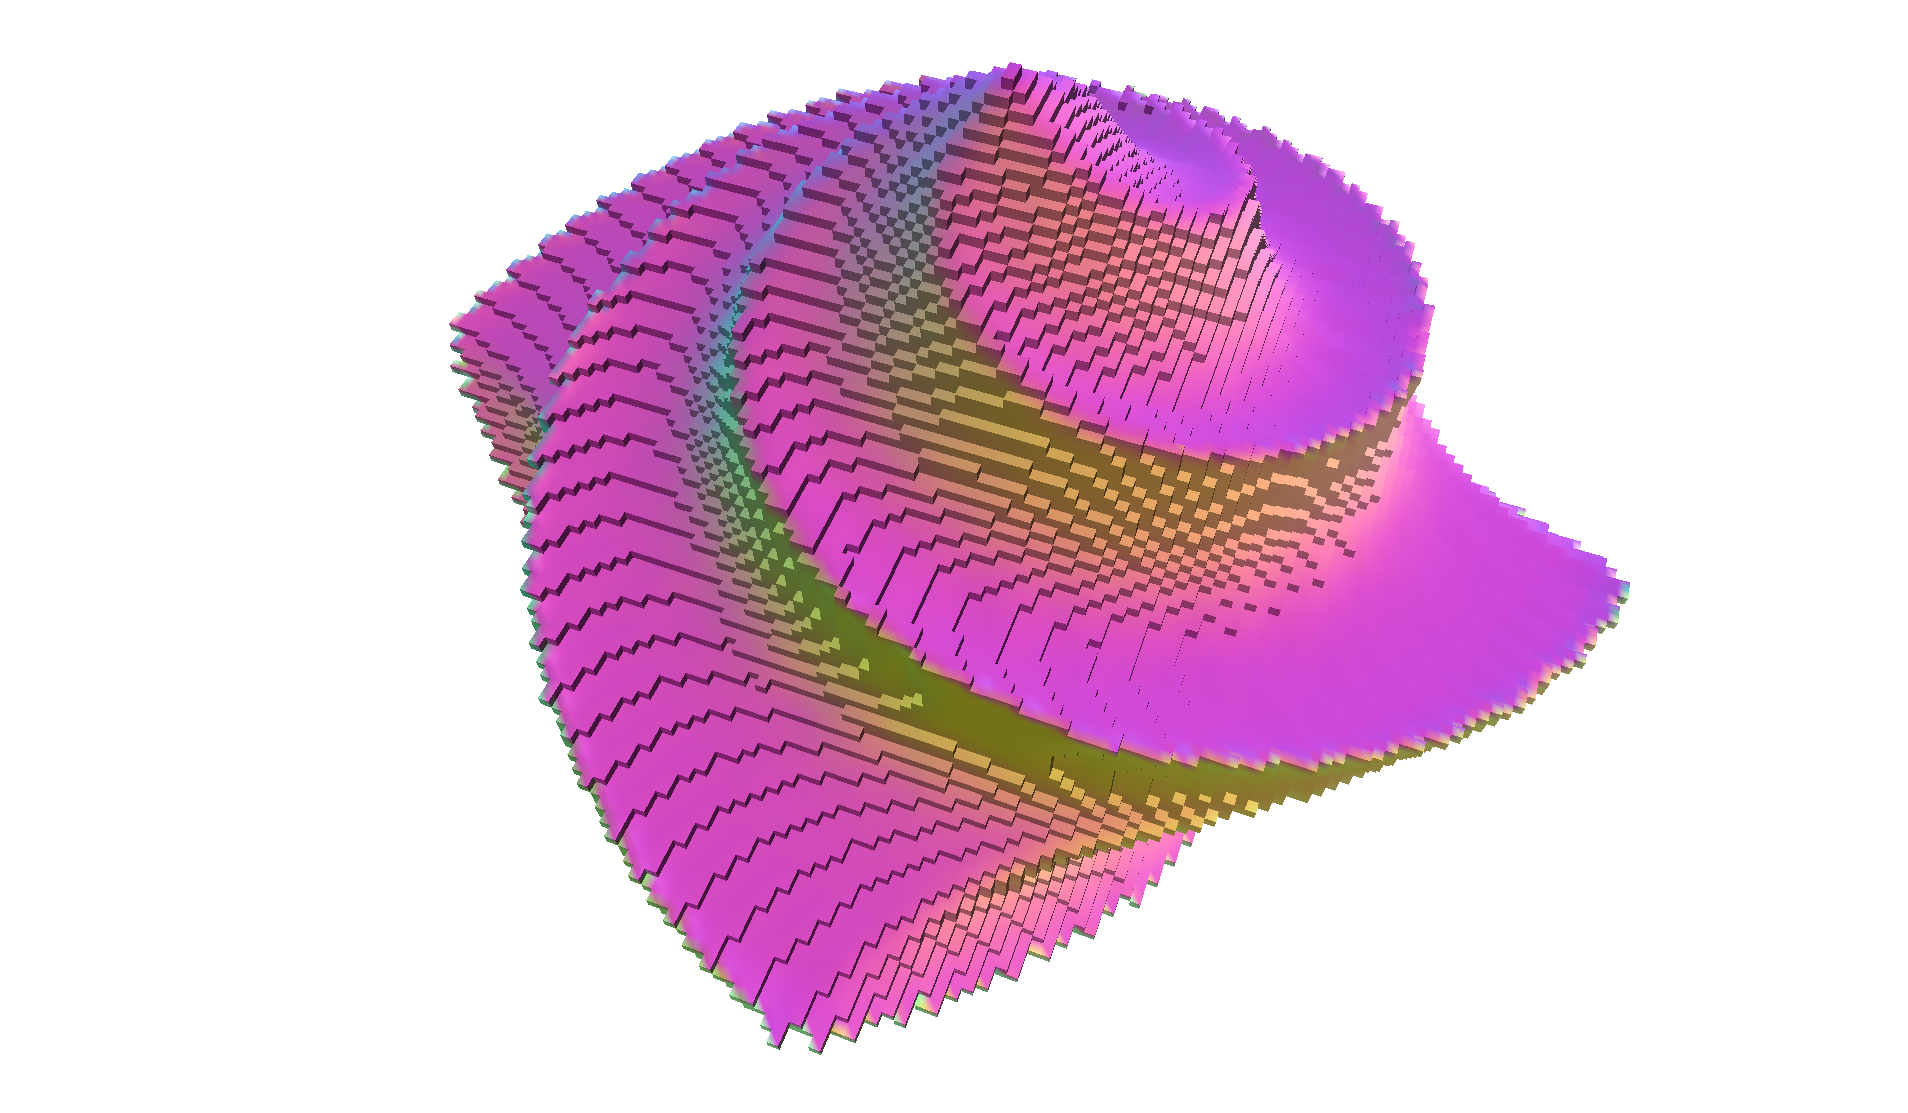
\includegraphics[width=0.4\textwidth]{pictures/octaflower-normal-estimation-cubes-II} &
            %% 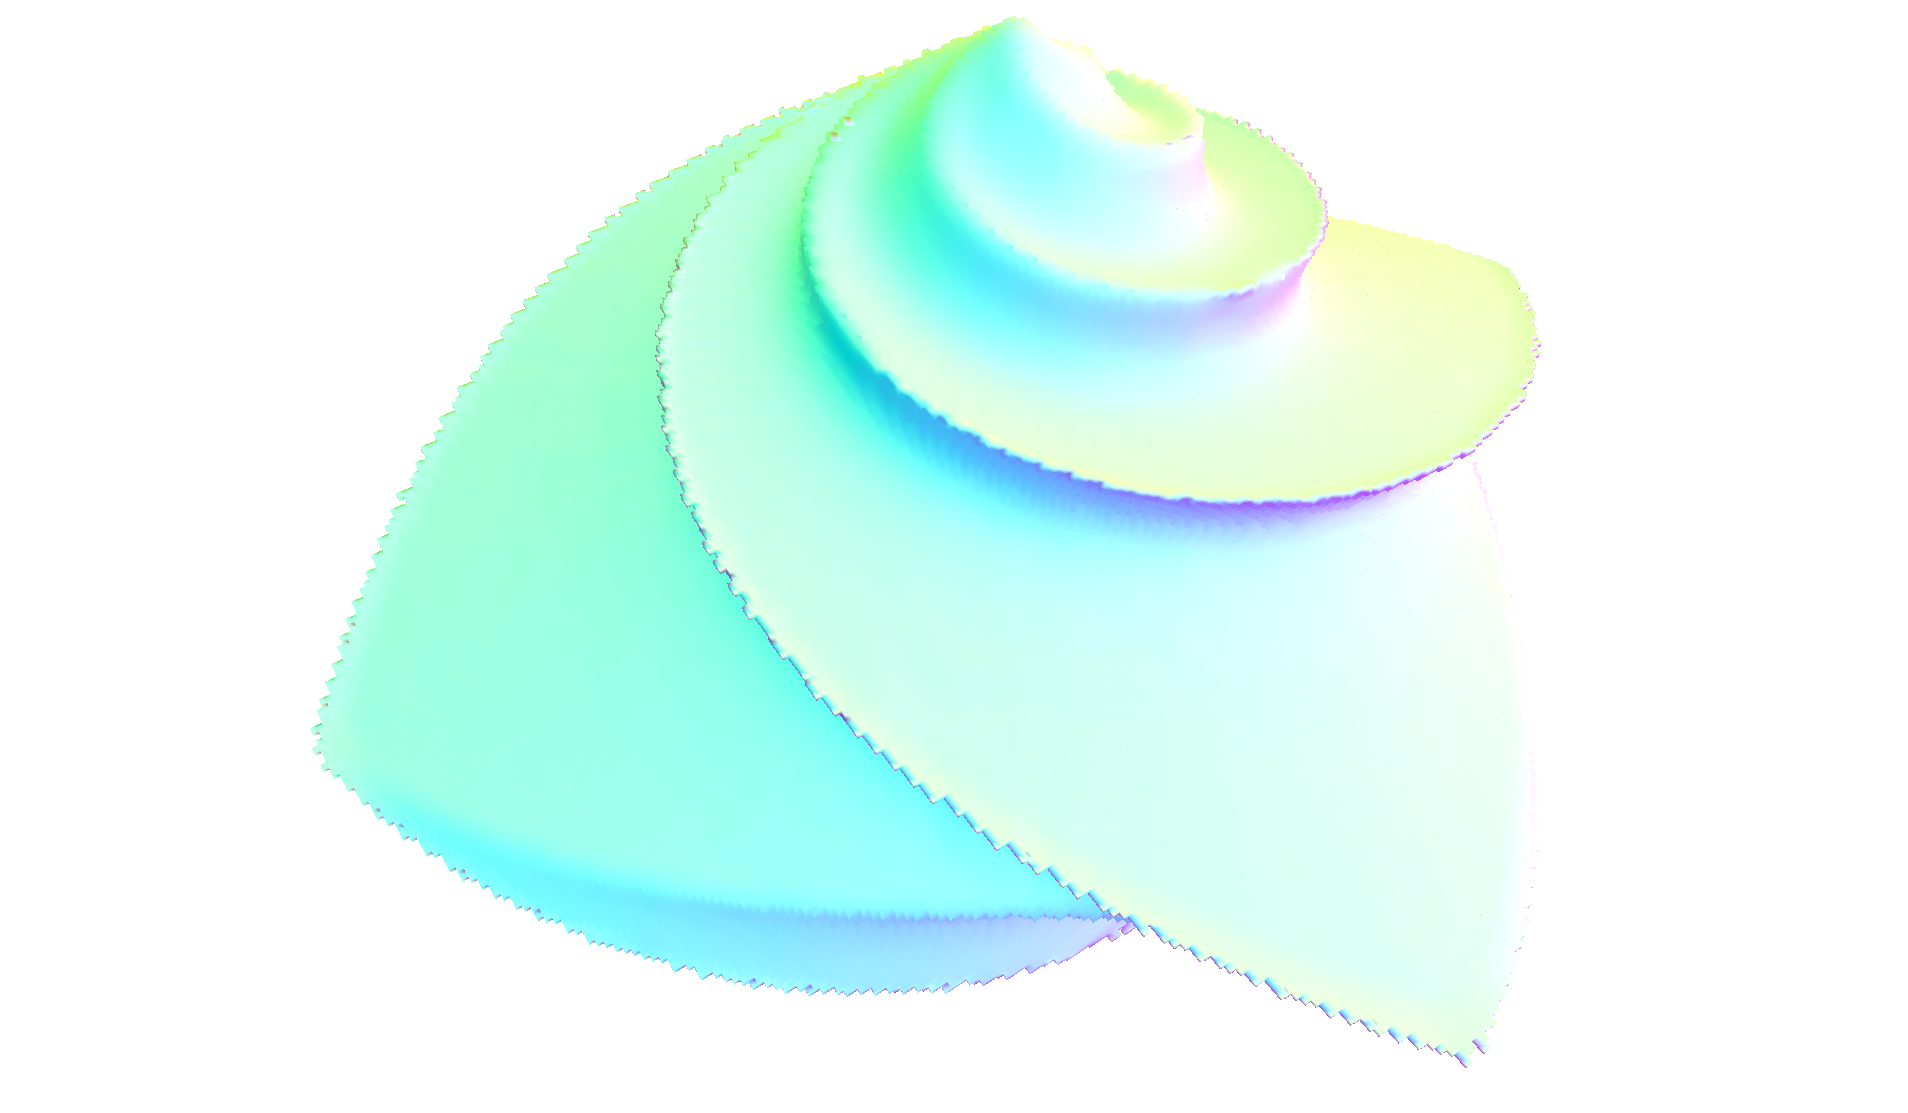
\includegraphics[width=0.4\textwidth]{pictures/octaflower-normal-estimation-smooth-II} \\
            \hline
            \raisebox{9mm}{Ours} &
            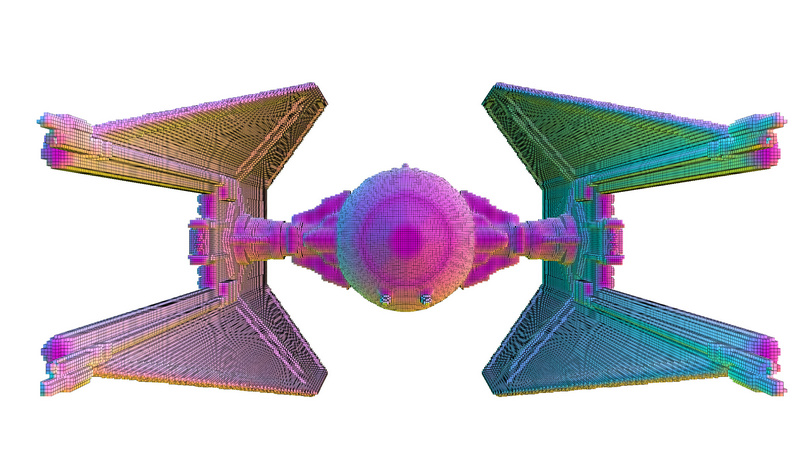
\includegraphics[width=0.33\textwidth]{pictures/tie256-VN-flat-edge-small} &
            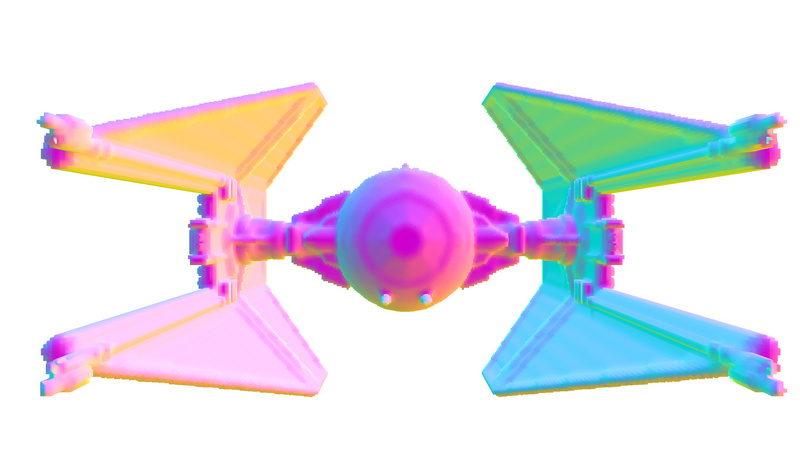
\includegraphics[width=0.33\textwidth]{pictures/tie256-VN-flat-small} \\
            %% 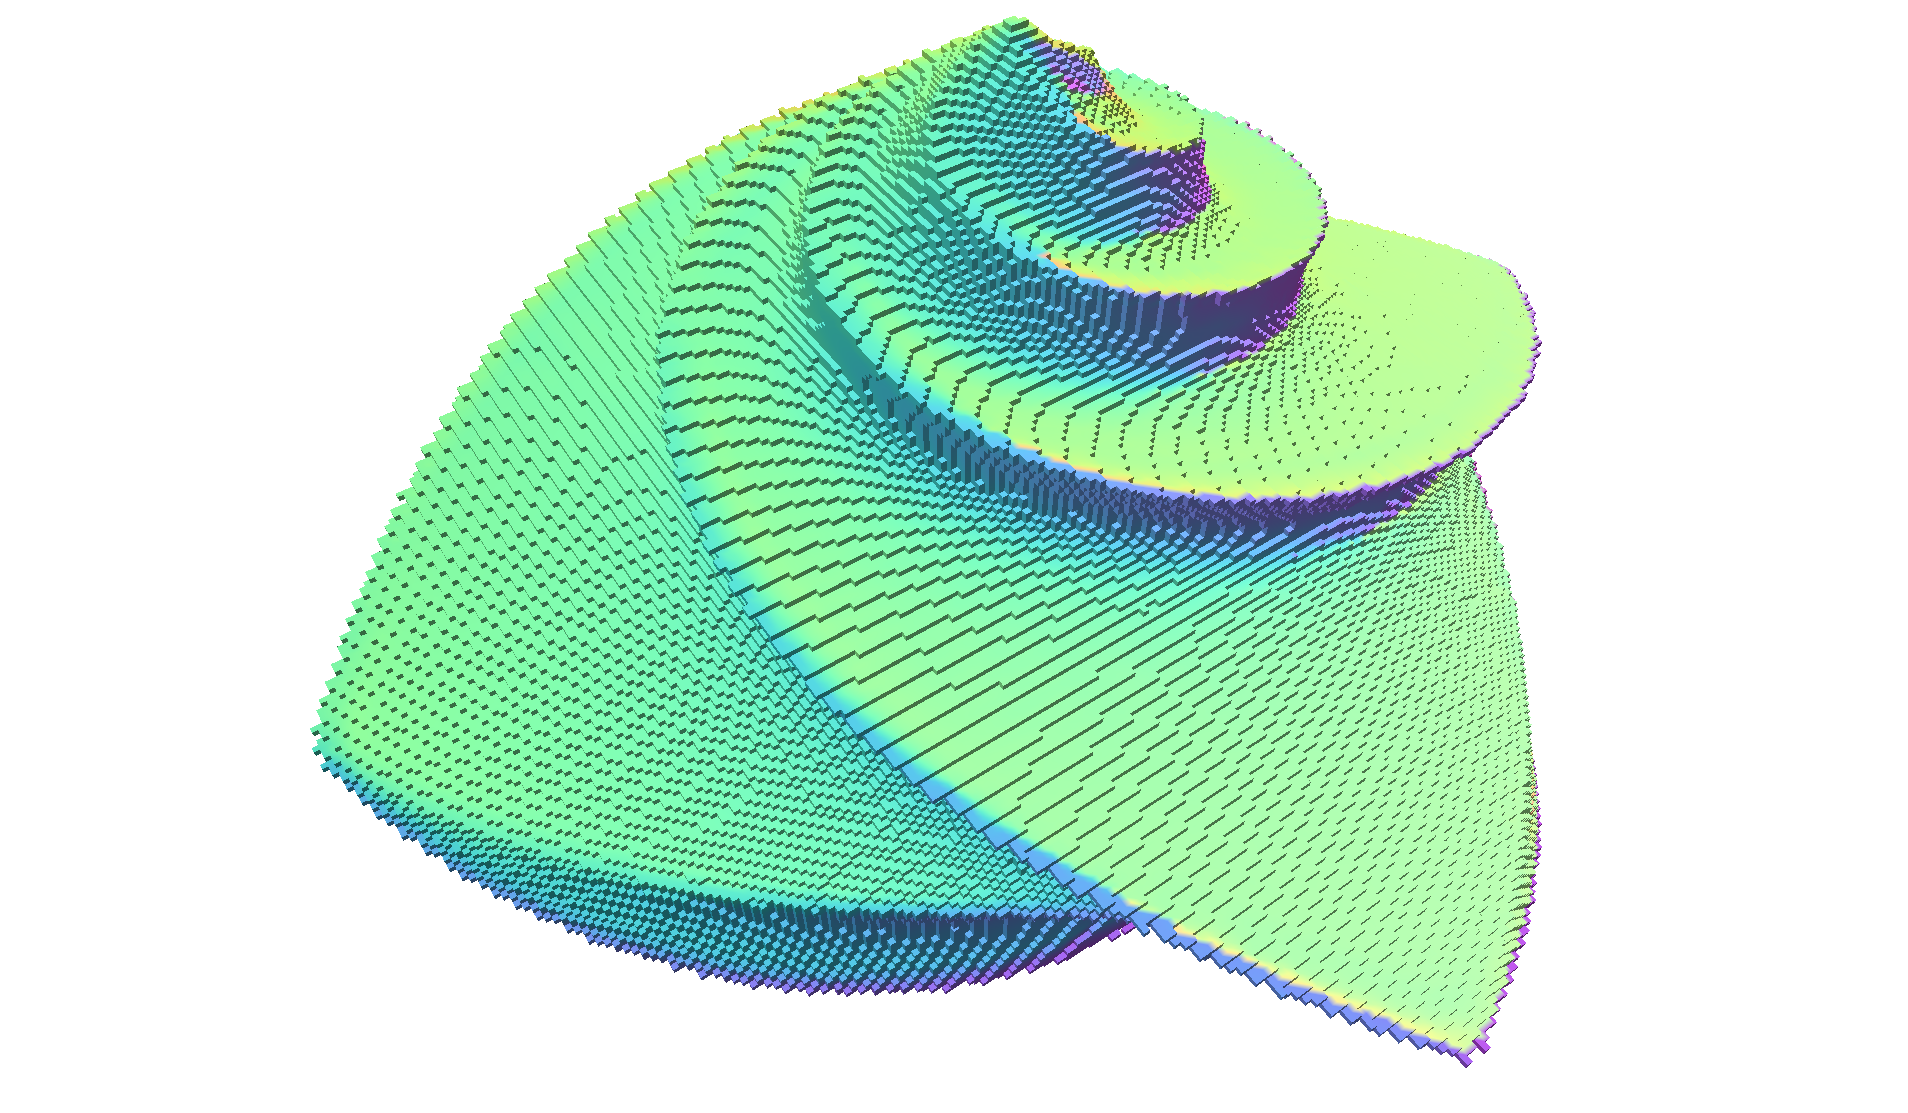
\includegraphics[width=0.4\textwidth]{pictures/octaflower-normal-estimation-cubes-NV} &
            %% 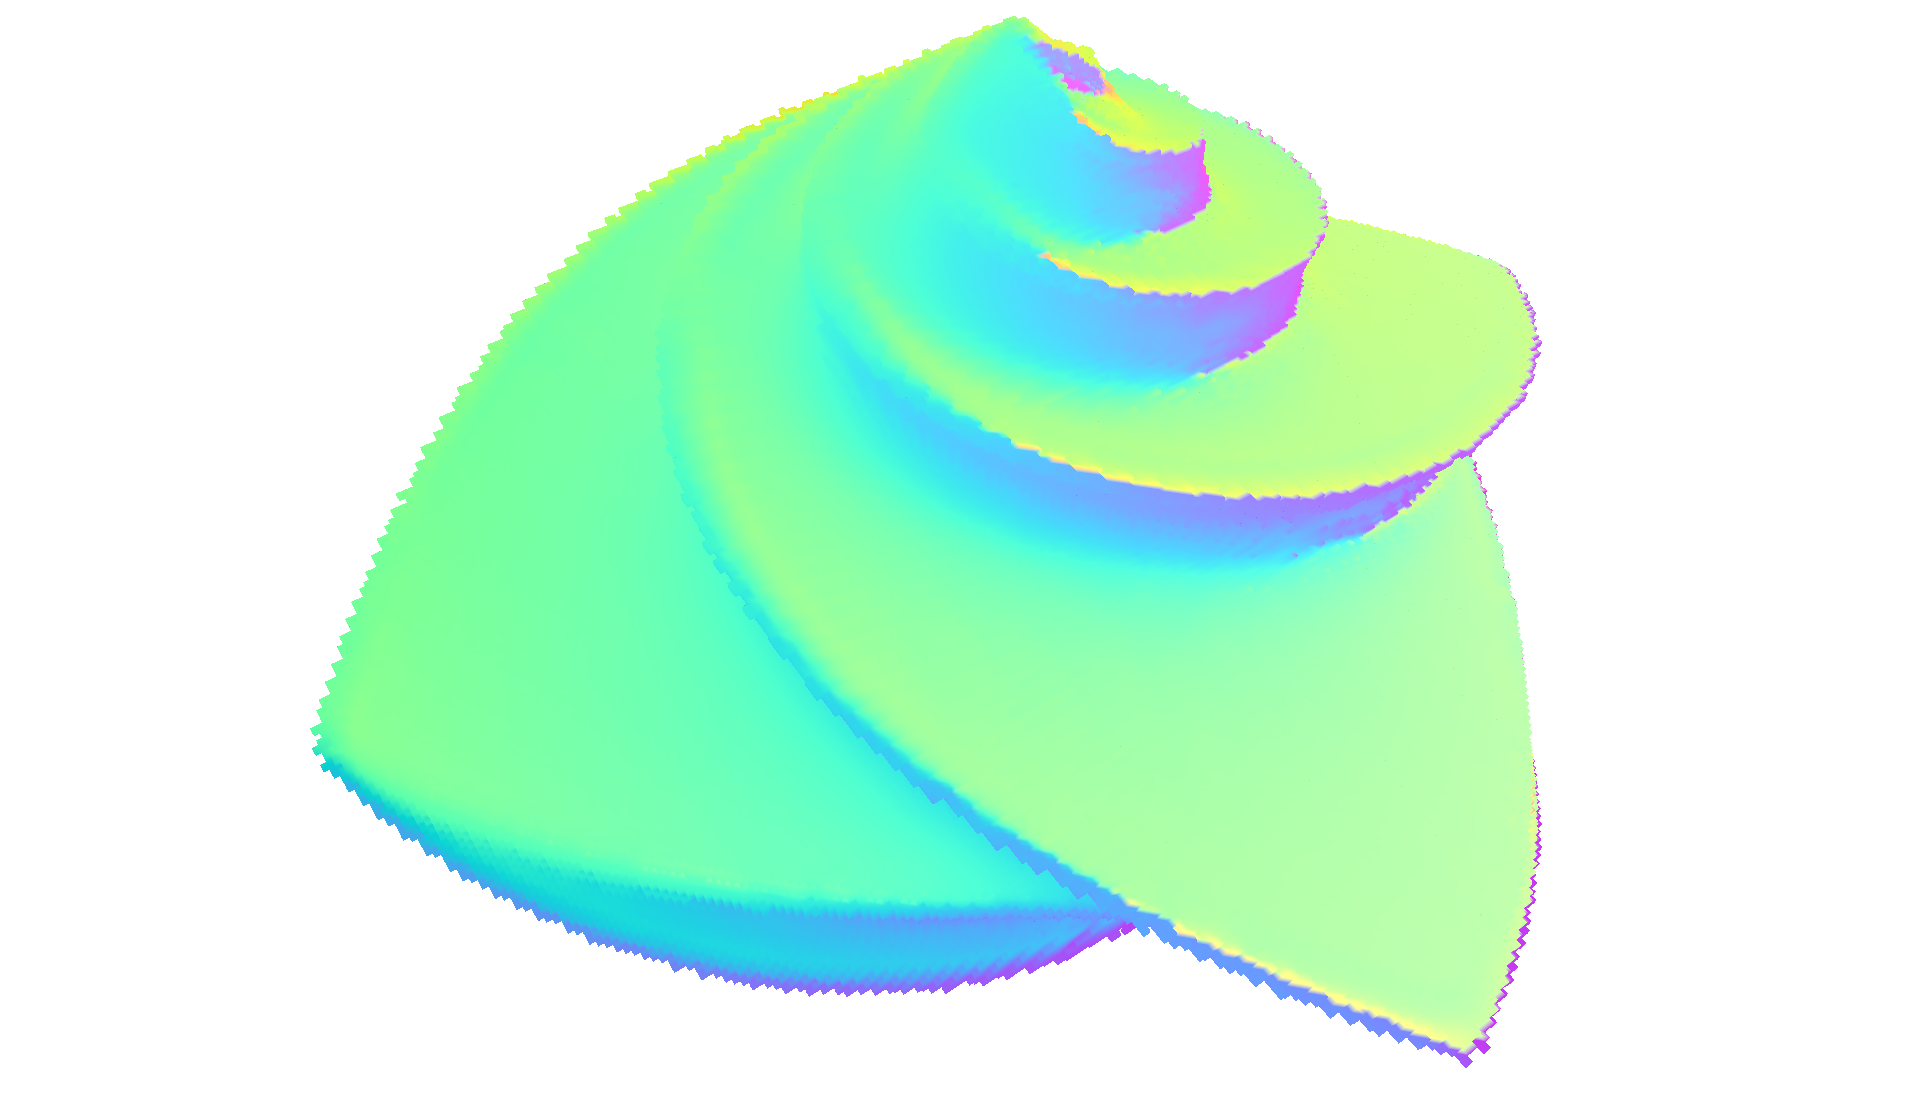
\includegraphics[width=0.4\textwidth]{pictures/octaflower-normal-estimation-smooth-NV} \\
            \hline
        \end{tabular}
    \end{frame}

    \begin{frame}{Curvature estimation using Corrected Normal Current (CNC) [Lachaud et al., 2022]}
        \centering
        \hspace*{-2.3em}
        \begin{tabular}{|c||c|c|c|}
            \hline
            Curv. & II & Convolved Triv. & Ours \\ \hline \hline
            \raisebox{18mm}{$H$} &
            \MyZoom{pictures/d20-H-II-small.jpg} &
            \MyZoom{pictures/d20-H-CTriv-small.jpg}&
            \MyZoom{pictures/d20-H-VN-small.jpg}\\ \hline
        \end{tabular}
    \end{frame}

    \begin{frame}{Curvature estimation using Corrected Normal Current (CNC) [Lachaud et al., 2022]}
        \centering
        \hspace*{-2.3em}
        \begin{tabular}{|c||c|c|c|}
            \hline
            Curv. & II & Convolved Triv. & Ours \\ \hline \hline
            \raisebox{18mm}{$G$} &
            \MyZoom{pictures/d20-G-II-small.jpg} &
            \MyZoom{pictures/d20-G-CTriv-small.jpg}&
            \MyZoom{pictures/d20-G-VN-small.jpg}\\ \hline
        \end{tabular}
    \end{frame}

    \begin{frame}{Conclusion}
        \begin{itemize}
            \item Improved normal and curvature estimation
            \item New efficient visibility computation method
            \item Simple data structure
            \item Parameter-free
            \item Salliency and Feature aware
        \end{itemize}
    \end{frame}

    \begin{frame}{Future works}
        \begin{itemize}
            \item GPU implementation (ongoing)
            \item Pattern detection
            \item Learning-based methods
            \item Convergence proof for the normal estimation algorithm depending on the gridsize
            \item Empirical study of the normal estimation convergence on piecewise smooth surfaces
        \end{itemize}
    \end{frame}

    \begin{frame}{Thank you for your attention!}
        \centering
        \Huge{Questions ?}
    \end{frame}
\end{document}
